\documentclass[10pt,a4paper]{report}
\usepackage[utf8]{inputenc}
\usepackage[german]{babel}
\usepackage{amsmath}
\usepackage{amsfonts}
\usepackage{amssymb}
\usepackage{tabularx}
\usepackage{graphicx}
\usepackage{wrapfig}
\usepackage{tikz}
\usepackage{gensymb}
\usepackage[normalem]{ulem}
\usepackage[version=3]{mhchem}
\usepackage[a4paper, left= 2cm, textwidth=17cm]{geometry}
\title{Pharmakologie Skriptum}

\newenvironment{reaction}{\begin{equation}}{\end{equation}}

\begin{document}
\maketitle

\tableofcontents
\chapter{Pharmakokinetik} Vorgänge nach oral Gabe eines Pharmakon
\begin{figure}[h]
	\centering 
	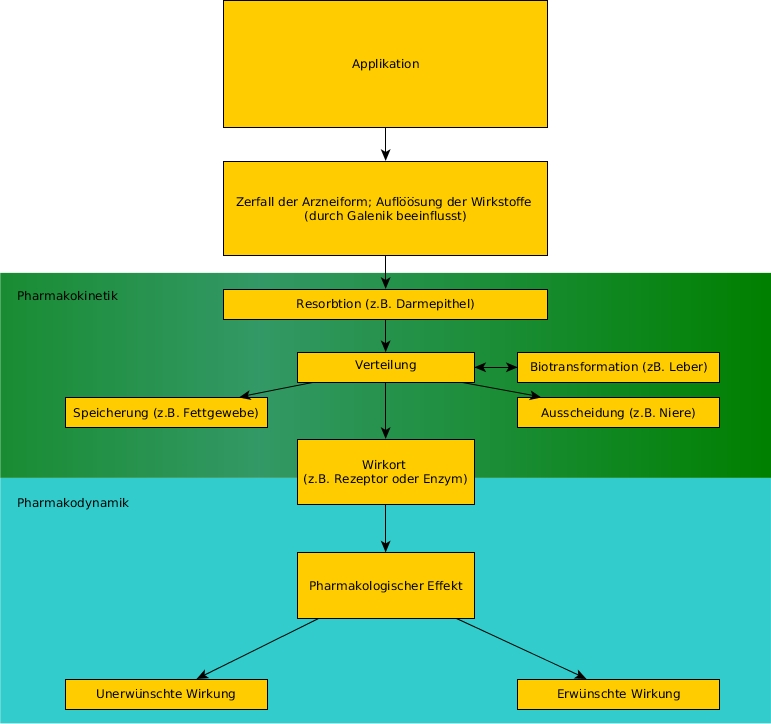
\includegraphics[width=0.6\textwidth]{Pharmakokinetik.jpg} 
	\caption{Pharmakokinetik/Pharmakodynamik} 
	\label{fig:Pharmakokinetik}
\end{figure}
\subsection{Definitionen}
\subsubsection{Pharmakon} biologisch wirksame Substanz (ohne Wertung)
		auch „Wirkstoff“; Wirkung erwünscht $\rightarrow$ Heilmittel;
					Wirkung unerwünscht  $\rightarrow$ Gift
\subsubsection{Arzneistoff} Pharmakon, das zur Vorbeugung, Linderung, Heilung oder 
Erkennung von Erkrankungen dienen kann
\subsubsection{Arzneimittel} zur Anwendung bei Mensch/Tier bestimmte Zubereitungsform eines Pharmakons nach der Zulassung
\subsection{Bezeichnung von Pharmaka}
\begin{enumerate}
	\item chemischer Name, Code-Nummer	\textit{4’-Hydroxyacetanilid}
	\item internationaler Freiname „generic name“	\textit{Paracetamol}
	\item Handelsname, Warenzeichen Benuron $^{\textregistered} $, Captin $ ^{\textregistered} $, Enelfa $^{\textregistered}$ 
	(25 Namen allein in Deutschl.)
\end{enumerate}
\subsection{Pharmakokinetik/Pharmakodynamik}
\subsubsection{Pharmakokinetik} 	Einflüsse des Organismus auf das Pharmakon (Resorption, Verteilung, Speicherung, Elimination)
\subsubsection{Pharmakodynamik} Einflüsse des Pharmakon auf den Organismus (Wirkmechanismus, zelluläre und system. Wirkung)
\subsubsection{Pharmakokinetik}  Vorgänge nach oraler Applikation eines Pharmakon
\subsubsection{Elimination} Prozesse, die zur Konzentrationsabnahme des Pharmakons im Körper führen
\begin{enumerate}
	\item Biotransformation / Metabolisierung
	\item Ausscheidung (Niere, Galle, Lunge)
\end{enumerate}
\subsection{Biotransformation / Metabolisierung}
\paragraph{Problem} lipophile, unpolare Pharmaka werden gut resorbiert, aber schlecht 	ausgeschieden. 
\paragraph{Lösung} Biotransformation zu hydrophilen Metaboliten v.a. in der Leber, Darm, Niere, Lunge u.a.

\subsubsection{Phase I: 	Funktionalisierungsreaktion}
Oxidation, Reduktion, Hydrolyse u.a. 
Einführung oder Freisetzung funktioneller, meist polarer Gruppen 

\begin{itemize}
\item Wirkung des Pharmakons wird beeinflusst
\item meist Voraussetzung für Phase II Reaktion
\end{itemize}
\subsubsection{Phase II: Konjugationsreaktion}
Glucuronidierung, Acetylierung, Sulfatierung, Methylierung u.a.. Kopplung von entsprechenden Resten an funktionelle Gruppe, die häufig in Phase I geschaffen wurde $\rightarrow$ Entstehung von meist biologisch inaktiven, gut wasserlöslichen Produkten, die problemlos ausgeschieden werden können.
\begin{figure}[h]
	\centering 
	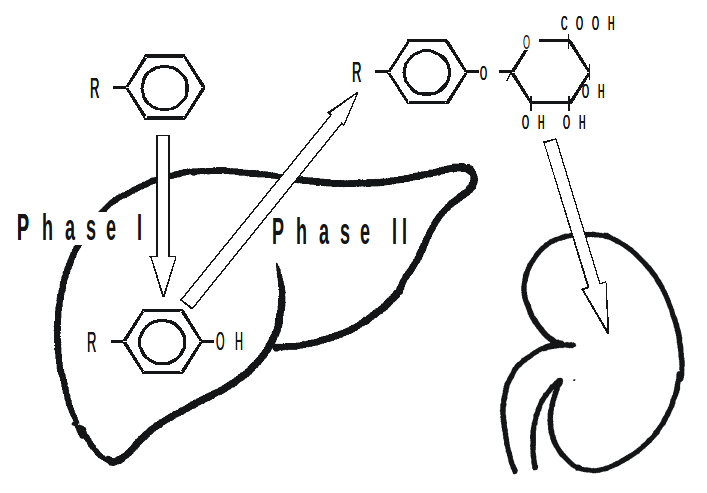
\includegraphics[width=0.4\textwidth]{Biotransformation.png} 
	\caption{Biotransformation} 
	\label{fig:Biotransformation}
\end{figure}

\subsubsection{Bedeutung von Arzneimittelmetabolisierungsprozessen}
\begin{itemize}
	\item Eliminationsmechanismus
	\item Arzneimittelinteraktionen durch Enzymhemmung oder Enzyminduktion
	\item Bildung aktiver oder toxischer Metabolite
	\item präsystemische Elimination oral verabreichter Pharmaka (first-pass-Effekt)
	\item genetisch bedingte individuelle Unterschiede der Arzneimittelelimination
\end{itemize}

\subsubsection{Für den Fremdstoffmetabolismus wichtige Vertreter aus der Superfamilie der humanen Cytochrom P450 Monooxygenasen (CYP)} \mbox{}\\

\begin{tabularx}{\textwidth}{X|XXXXX}
  Name & Vorkommen & typische Substrate & Induktoren & Inhibitoren	& Bemerkungen \\\hline \hline
  CYP1A1&intestinal, pulmonal&arom. Kohlenwasserstoffe, Paracetamol&arom. Kohlenwasserstoffe, via Ah-Rezeptor&Chinole&mögliche Bedeutung bei Biotoxinfizierung von Präkanzerogenen \\
  CYP1A2&hepatisch&Coffein, Theophyllin&arom. Kohlenwasserstoffe via Ah-Rezeptor (z.B. Tabakrauch)&&mögliche Bedeutung bei Biotoxinfizierung von Präkanzerogenen \\
  CYP2B6&hepatisch&Cyclophosphamid&Cyclophosphamid, Phenobarbital&&\\
  CYP2C9/19&hepatisch, intestinal&Phenytoin, Wafarin, Omeprazol&Barbiturate, Rifampicin&Cimetidin&ca. 20\% aller Pharmaka\\
  CYP2D6&hepatisch intestinal renal& $\beta$-Blocker Antiarrhythmika Antidepressiva Neuroleptika&&Chinidin SSRI (z.B. Fluoxetin)& ca. 25\% aller Pharmaka, 40\% aller Allele defekt\\
  CYP2E1&hepatisch intestinal Leukozyten&Ethanol Nitrosamine&Ethanol Isoniazid& Disolfiram& ca. 15\% aller Pharmaka Biotoxifizierung?\\
  CYP3A4&hepatisch intestinal& Ciclosporin Nifedipin Terfendadin Ethindylestradiol HIV-Proteaseh. Statine&Rifampicin Carbamazepin Phenytoin Phenobarbital Hyperforin (Johanniskraut)& Azol-Antimykotika Naringin (Grapefruitsaft) HIV-Proteaseh. Makrolide& ca. 40-50\% aller Pharmaka\\ \hline  
\end{tabularx}
\begin{figure}[h]
	\centering 
	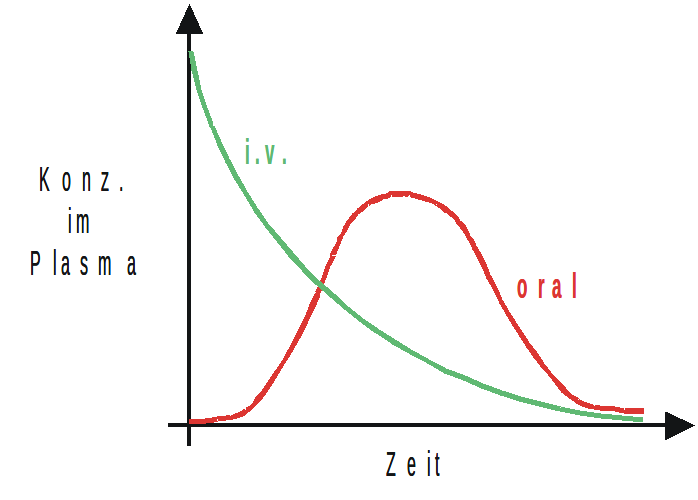
\includegraphics[width=0.4\textwidth]{konzentrationzeit.png} 
	\caption{Bioverfügbarkeit} 
	\label{fig:Bioverfuegbarkeit}
\end{figure}
\subsubsection{Mechanismen der Induktion von Cytochrom P450 Monooxygenasen} \mbox{}\\
\begin{figure}[h]
	\centering 
	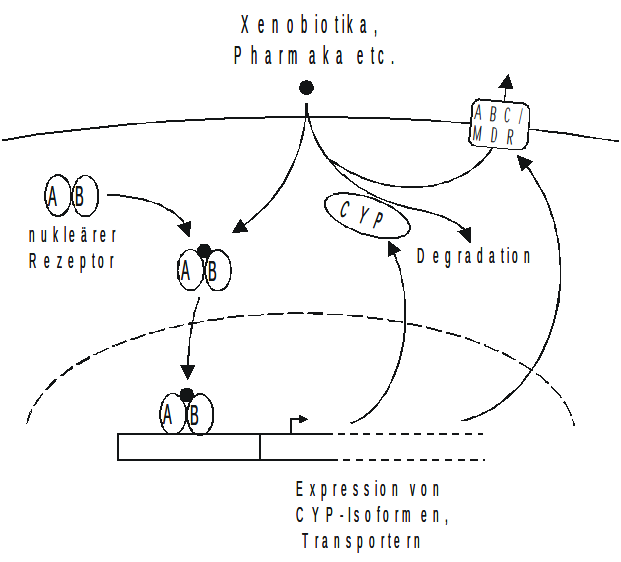
\includegraphics[width=0.4\textwidth]{CYP2.png} 
	\caption{Induktion von Cytochrom P450 Monooxygenasen} 
	\label{fig:Cytochrom2}
\end{figure}
\begin{tabularx}{\textwidth}{XXXX}
Xenobiotikum Pharmakon& nukleärer Rezeptor (A/B)&induz. Enzym / Transporter&Enzymubstrate\\\hline
Dioxin, aromat. Hydrocarbone (Rauchen)& Ah-Rezeptor/ARNT&CYP1A1 CYP1A2&aromat. Hydrocarbone, Coffein, Theophyllin; \textit{nicht} Dioxin!\\
Barbiturate&CAR/RXR&CYP2B,C ABCC3&viele Pharmaka\\
Rifampicin, Hyperforin, Paclitaxel, u.a.&PXR/RXR&CYP3A/2C)/ MDR-1, ABCB1, C2&viele Pharmaka\\
Fibrate&PPAR$\alpha$/RXR&CYP4A1,3&\\
\end{tabularx}
\subsubsection{Beispiele für Arzneimittelinteraktionen 
durch Enzymhemmung und -induktion} \mbox{}\\
\paragraph{Enzyminduktion}
\begin{itemize}
	\item Induktion von CYP1A1/2 bei Rauchern $\rightarrow$ Abbau von Theophyllin und Coffein $\uparrow$
	\item Induktion von CYP3A4 durch Rifampicin, Johanniskraut, Phenytoin u.a. 
	\begin{itemize}%[leftmargin=1em]
  \renewcommand{\labelitemi}{$\rightarrow$}
 \item Abbau von Ethinylestradiol $\uparrow$ („Pillenversager“)
 \item Abbau von Ciclosporin (Transplantat-Abstoßung) etc.
\end{itemize}
\end{itemize}
\paragraph{Enzymhemmung}
\begin{itemize}
	\item Hemmung von CYP2D6 durch Selektive Serotonin-„Reuptake“-Hemmer (z.B. Fluoxetin)
	\begin{itemize}
	\renewcommand{\labelitemi}{$\rightarrow$}
	\item verminderter	 Abbau von Antidepressiva, Neuroleptika
	\end{itemize}
	\item Hemmung von CYP3A4 durch Azol-Antimykotika oder Grapefruitsaft u.v.a.
	\begin{itemize}
		\renewcommand{\labelitemi}{$\rightarrow$}
		\item verminderter Abbau von Ciclosporin ($\rightarrow$ Nephrotoxizität) 
	     oder Terfenadin, Cisaprid ($\rightarrow$ Herzrhythmusstörungen) oder Statinen ($\rightarrow$ Myopathie)
	\end{itemize}
\end{itemize}
\subsubsection{Phase II Reaktionen} \mbox{}\\
\paragraph{Glucuronosyltransferasen}
\begin{itemize}
	\item ca. 40\% aller Pharmaka
	\item Uridindiphosphat-Glucuronosyltransferasen (UGT)
	\item 17 Isoformen, mikrosomal; Leber, Darmepithel, Niere
\end{itemize}
\paragraph{Glutathion-S-Transferase (GST)}
\begin{itemize}
	\item ca. 10\% aller Pharmaka
\end{itemize}
\paragraph{N-Acetyltransferase (NAT) }
\begin{itemize}
	\item ca. 10\% aller Pharmaka
	\item 2 Isoformen (NAT I und NAT II); NAT II Polymorphismus
\end{itemize}
\paragraph{Sulfotransferase (SULT)}
\begin{itemize}
	\item ca. 20\% aller Pharmaka
	\item Transfer eines Sulfat-Restes aus 
	dem Kosubstrat PAPS
\end{itemize}
\paragraph{Methyltransferase}
\begin{itemize}
	\item Methylgruppentransfer aus S-Adenosylmethionin
\end{itemize}
\subsubsection{Bildung aktiver oder toxischer Metabolite (Beispiele)} \mbox{} \\
\begin{figure}[h]
	\centering 
	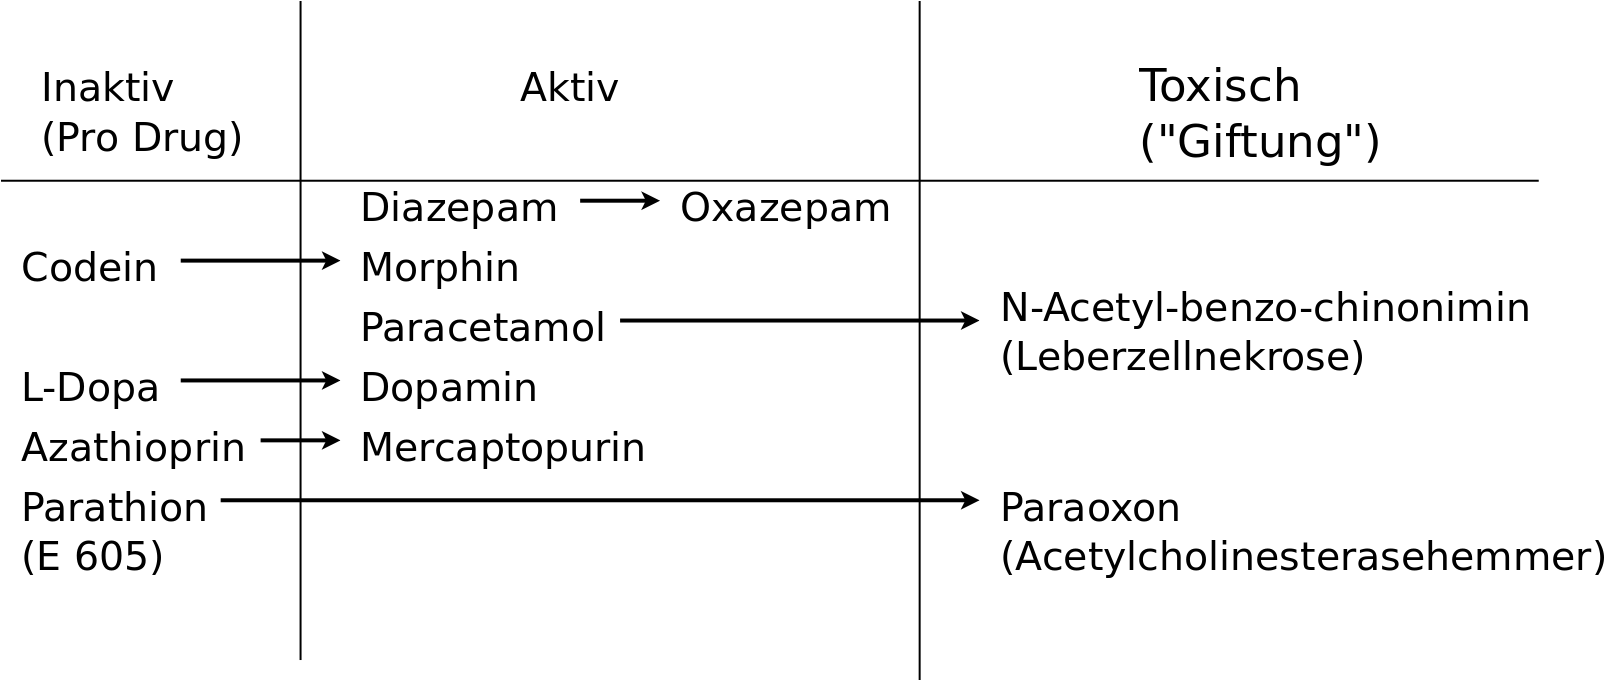
\includegraphics[width=0.5\textwidth]{Pharmakodynamik.png} 
	\caption{Bildung aktiver oder toxischer Metabolite (Beispiele)} 
	\label{fig:Metabolite}
\end{figure}
\subsubsection{First-Pass-Effekt} \mbox{} \\
enteral resorbierte Pharmaka gelangen nach Passage der Darmwand über die Pfortader zuerst in die Leber, danach in die systemische Zirkulation \textit{First-Pass-Effekt}: Anteil eines Pharmakons, der bei Passage der Darmwand und Leber metabolisiert 
oder zurückgehalten wird hoher first-pass-Effekt: z.B. Glyceroltrinitrat, Lidocain
\begin{figure}[h]
	\centering 
	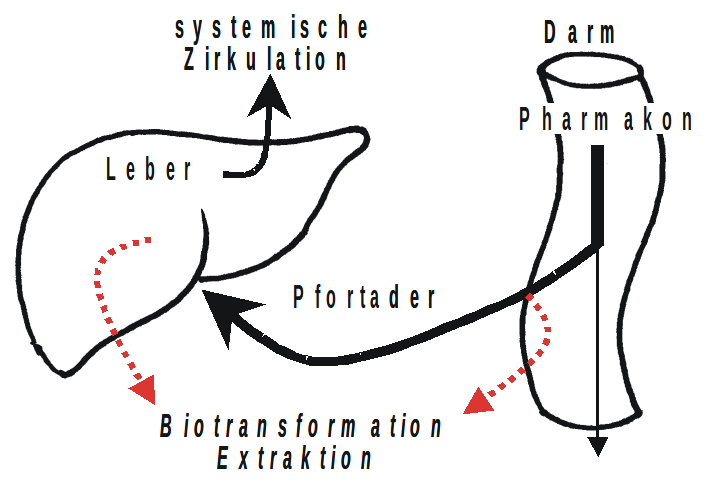
\includegraphics[width=0.4\textwidth]{firstpass.png} 
	\caption{First-Pass-Effekt} 
	\label{fig:FirstPass}
\end{figure}
\subsection{Pharmakogenetik / Genetisch bedingte Unterschiede in der Metabolisierung von Pharmaka (Beispiele)} \mbox{} \\
\begin{figure}[h]
	\centering 
	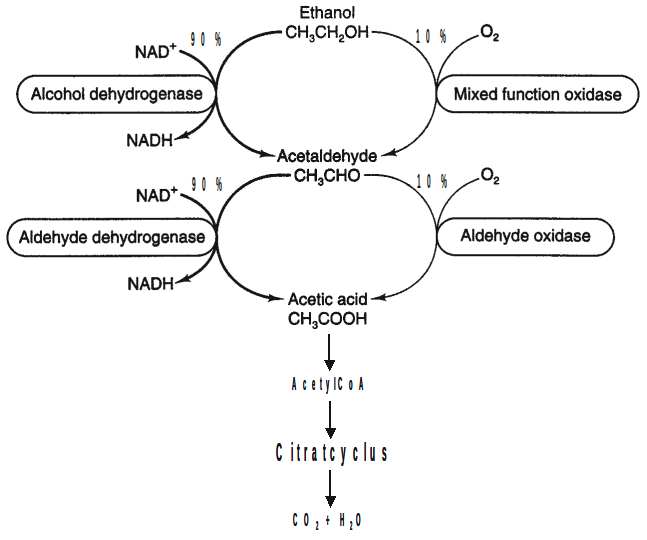
\includegraphics[width=0.4\textwidth]{ethanolbiotransformation.png} 
	\caption{Ethanol Biotransformation} 
	\label{fig:EthanolBiotransformation}
\end{figure}
\subsubsection{Phase I} 
\textit{Aldehyd-Dehydrogenase 2}: inaktive Variante bei 50\% der Asiaten $\rightarrow$ Abbau von Äthanol $\downarrow$\\ \\
\textit{CYP2D6} 	inaktive Variante bei 8\% der Europäer „PM, poor metabolizer“ vs. „EM, extensive metabolizer“ Abbau von $\beta$-Blockern, Antidepressiva, Antiarrhythmika u.a. $\downarrow$
\subsubsection{Phase II}
\textit{N-Acetyltransferase (NAT II)}		„langsam Acetylierer“ vs. „schnell Acetylierer (je 50\% bei Europäern)$\rightarrow$ Abbau von Isoniazid u.a. $\downarrow$
\subsection{Ausscheidung} \mbox{} \\
v.a. renal, biliär/intestinal, pulmonal
\subsubsection{renal}
(häufigster Ausscheidungsweg)
\begin{itemize}
	\item glomeruläre Filtration bis Molmasse von ca. 15.000-20.000
	\item tubuläre Rückresorption lipophile Stoffe: gut; hydrophile Stoffe: schlecht Basen und Säuren: pH-abhängig
	\item tubuläre Sekretion: aktiver Prozeß im proximalen Tubulus; Transportsystem für organische Säuren z.B. Harnsäure, Penicillin G (u.a. MRP2) Transportsystem für organische Basen z.B. Dopamin (u.a. MDR1), organ. Anionen (z.B.: Thiazide)
\end{itemize}
Allgemein: Renale Ausscheidung $\downarrow$ bei Niereninsuffizienz und im Alter
\subsubsection{bilär/intestinal} häufig Metabolite mit Molmassen $>$500 z.B. Tetracycline, Digitoxin-Metabolite
\textit{enterohepatischer Kreislauf} Intestinale Ausscheidung
\subsubsection{pulmonal}
z.B. Inhalationsanästhetika
\subsection{Elimination von Pharmaka} \mbox{} \\
\begin{figure}[h]
	\centering 
	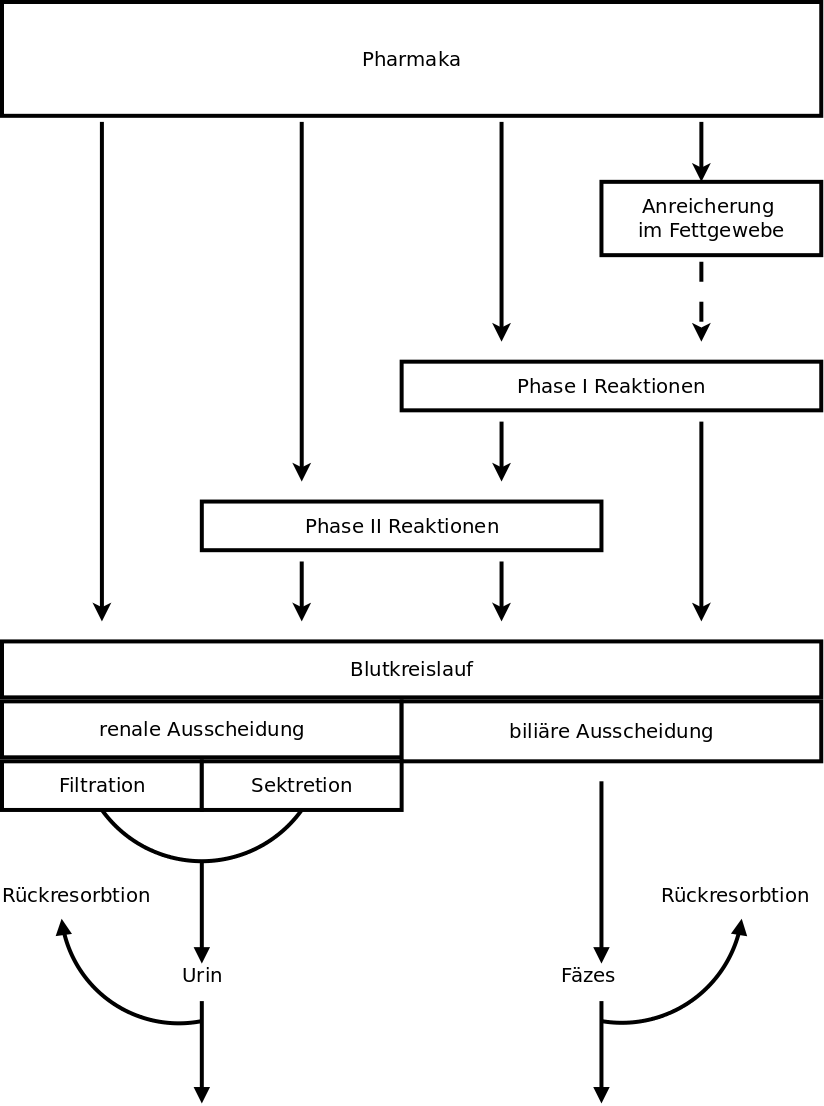
\includegraphics[width=0.4\textwidth]{Elimination.png} 
	\caption{Elimination} 
	\label{fig:Elimination}
\end{figure}
\subsection{Pharmakokinetische Parameter} \mbox{} \\
\subsubsection{Bioververfügbarkeit}
Der Anteil eines Pharmakons, der unverändert ins systemische Blut (großer Kreislauf) gelangt
Bei i.v.-Gabe: 100\%\\
\paragraph{Bei oraler gabe abhängig von:} Wirkstofffreisetzung,	Resorptionsquote, First-Pass-Effekt\\
\paragraph{„area under the curve” (AUC):}
AUC repräsentiert die Substanzmenge, 
die in das systemische Blut gelangt 
(unabhängig von der Resorptionsgeschwindigkeit)\\
AUC ist ein Maß für die Bioverfügbarkeit  $f=\frac{AUC_x}{AUC_{i.v.}}*100[\%]$
\begin{figure}[h]
	\centering 
	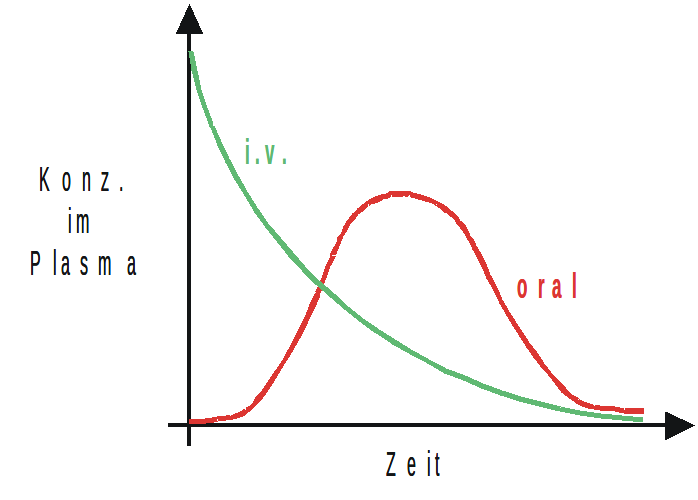
\includegraphics[width=0.4\textwidth]{konzentrationzeit.png} 
	\caption{Bioverfügbarkeit} 
	\label{fig:Bioverfuegbarkeit}
\end{figure}
\subsubsection{Verteilungsvolumen}
 fiktives Volumen, in dem sich ein Pharmakon verteilen würde, wenn es die gleiche Konzentration wie im Plasma hätte $V=\frac{Menge des Pharmakon im Organismus}{Plasmakonzentration}$ Das Verteilungsvolumen ist ein \textit{Proportionalitätsfaktor} zwischen der im Körper vorhandenen Menge und der Plasmakonzentration
 \subsubsection{Clearance}
 Plasmavolumen, das pro Zeiteinheit von einem Pharmakon befreit wird  $\rightarrow$ Maß für die Eliminationsleistung $CL=\frac{Menge eines Pharmakons, die pro Zeiteinheit eliminiert wird}{Plasmakonzentration}$
\begin{figure}[h]
	\centering 
	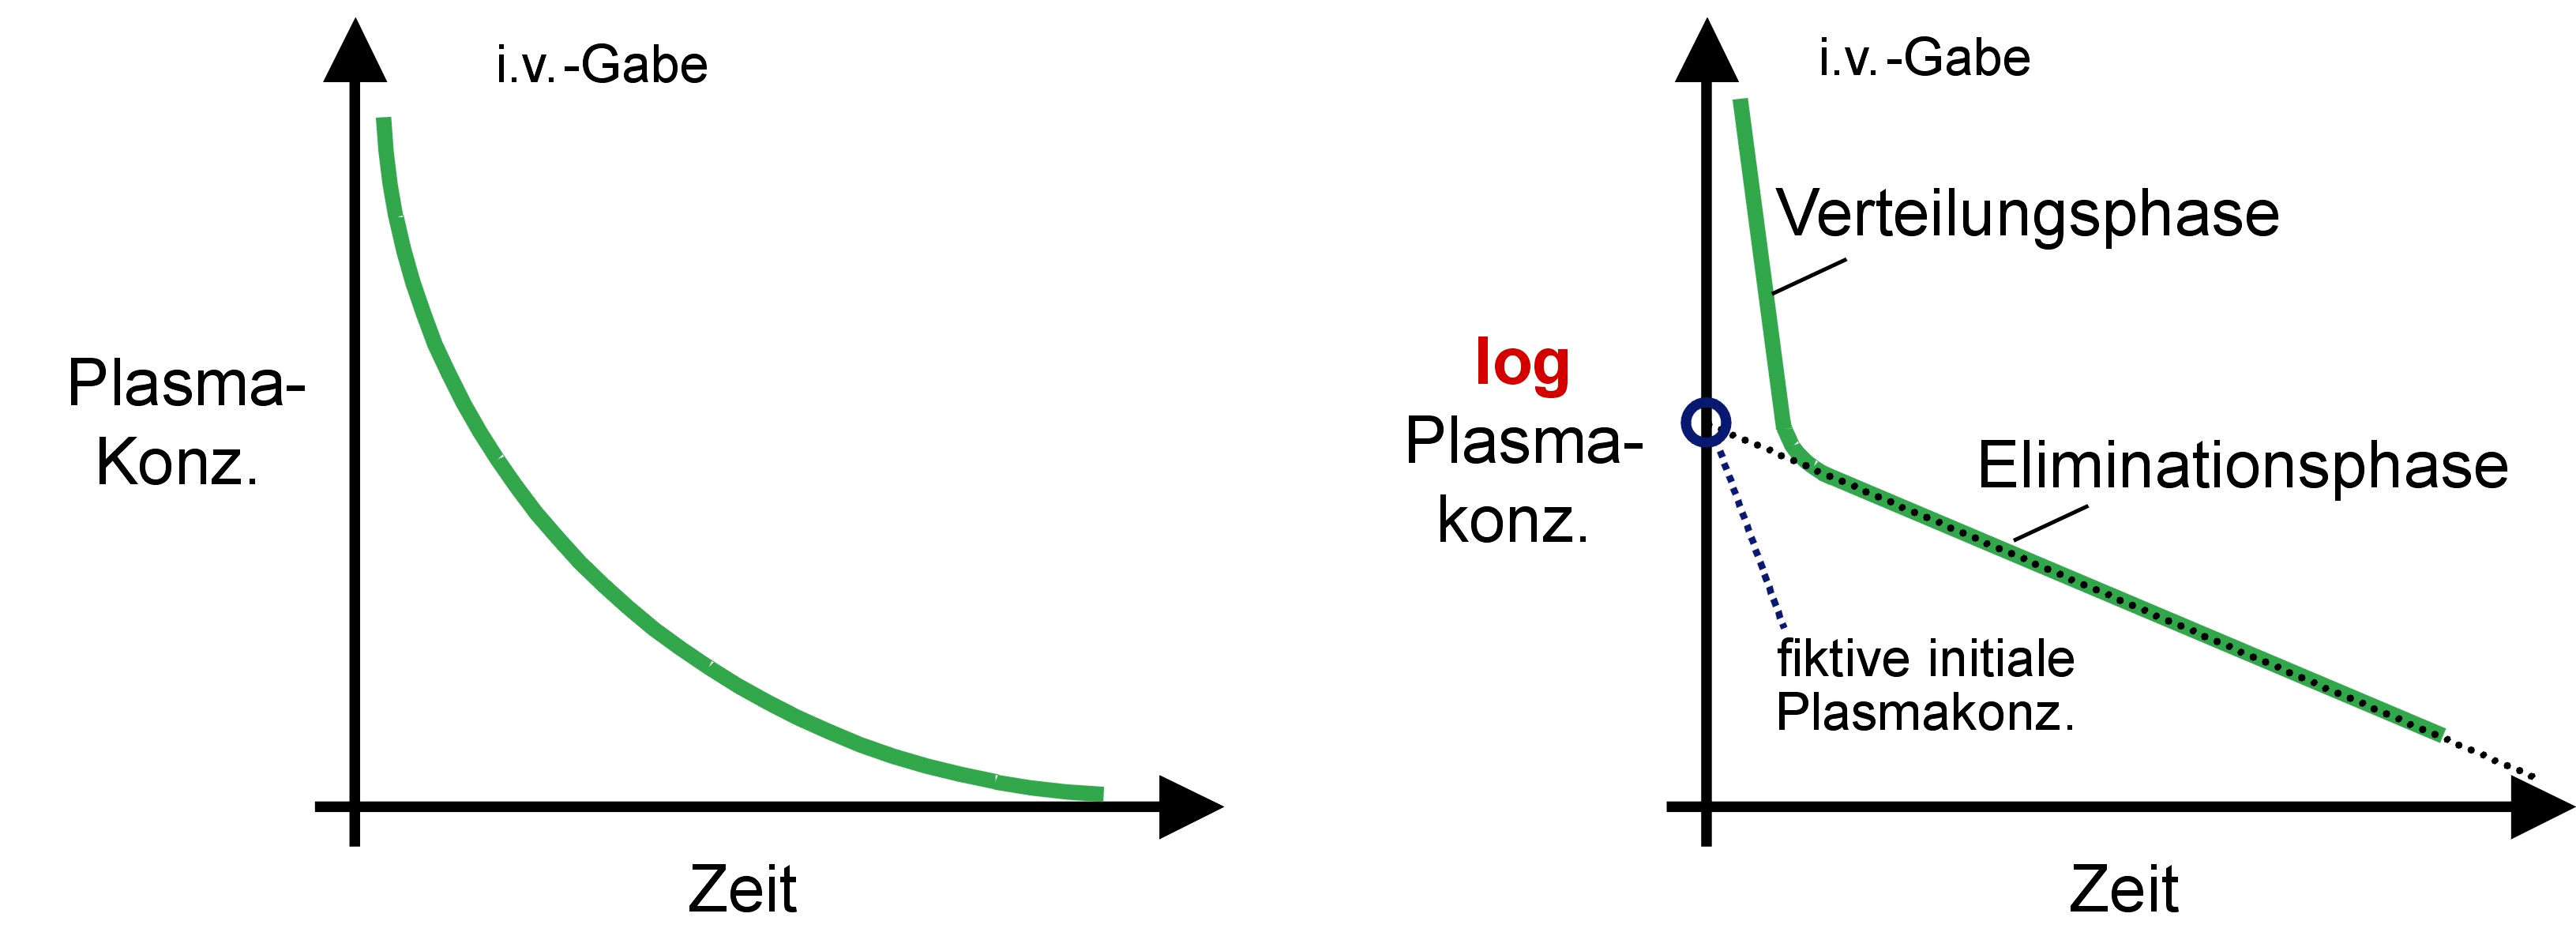
\includegraphics[width=0.4\textwidth]{clearance.png} 
	\caption{Clearance} 
	\label{fig:Clearance}
\end{figure}
\subsubsection{Plasmahalbwertszeit $t_{\frac{1}{2}}$} Zeit, in der die Plasmakonzentration auf die Hälfte des ursprünglichen Wertes abfällt.
\begin{figure}[!htb]\centering
   \begin{minipage}{0.49\textwidth}
     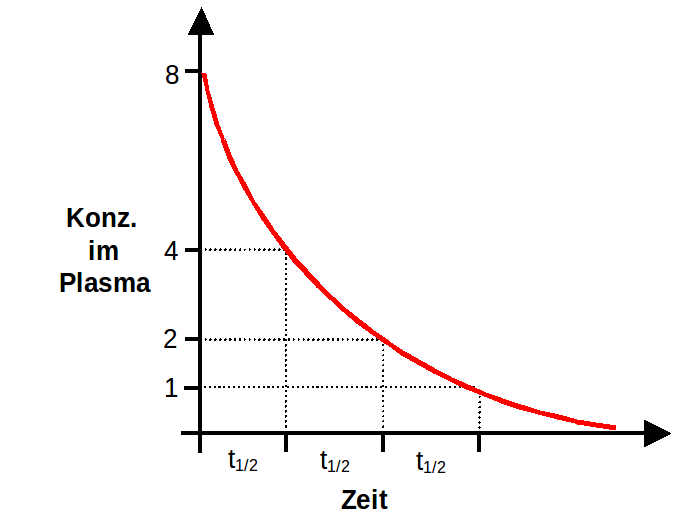
\includegraphics[width=\linewidth]{kinetik0.png}
     \caption{Kinetik 0. Ordnung: (häufig !) Eliminationsgeschwindigkeitist proportional 	zur jeweiligen Plasmakonzentration, 
Exponentialfunktion}\label{Fig:kinetik0}
   \end{minipage}
   \begin {minipage}{0.49\textwidth}
     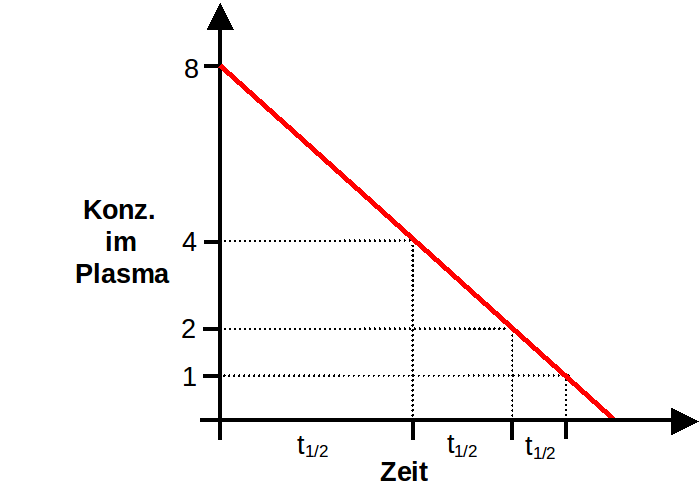
\includegraphics[width=\linewidth]{kinetik1.png}
     \caption{Kinetik 1. Ordung: (selten)
Eliminationsgeschwindigkeit ist konstant
z.B. durch Sättigung des abbauenden Enzyms}\label{Fig:kinetik1}
   \end{minipage}
\end{figure}
\subsubsection{Kinetik nach wiederholter Gabe}
Konz. im Körper abhängig von:- Dosis, - Dosierintervall, - Eliminations-HWZ \\
\paragraph{Kumulation}  Wirkstoffzunahme nach wiederholter Gabe; abhängig vom relativen Dosierintervall ($\epsilon$); $\epsilon=\frac{Dosierintervall(\tau)}{Eliminations-HWZ}$ ($t_{\frac{1}{2}}$);$\epsilon <1$ $\rightarrow$  Gefahr der Kumulation (z.B. Pharmaka mit langer $t_{\frac{1}{2}}$; Digitoxin, Cumarine u.a.) 


\chapter{Pharmakodynamik}
\section{Angriffsorte von Pharmaka}
\subsection{Fremdorganismus / Mikroorganismus}
(Bakterium, Virus, Pilz, Parasit)
\subsection{Menschlicher / tierischer Organismus (Makroorganismus)}
\subsubsection{Extrazellulär}
\begin{enumerate}
	\item physikalisch wirksam: Laxantien, osmotische 	Diuretika,Plasmaexpander
	\item chemisch wirksam: Antazida, Chelatbildner, Protaminsulfat (bindet Heparin), Ionenaustauscher wie Cholestyramin (bindet Gallensäuren)
	\item enzymatisch wirksam: tPA (Fibrinolyse), Enzym-Substitution
\end{enumerate}
\subsubsection{Zellulär}
\begin{enumerate}
	\item Zytoskelett z.B.: Vincaalkoloide (Zytostatika), Colchizin 
	\item DNS z.B.: Alkylantien (Zytostatika)
	\item Transporter z.B.: 
Noradrenalin-/Serotonin-Transporter (Antidepressiva) Ionentransporter (Diuretika); Protonenpumpe (Omeprazol)
	\item Ionenkanäle z.B.: 
	Spannungsabhängiger $Na^+$-Kanal (Lokalanästhetika)
	Spannungsabh. $Ca^{2+}$-Kanal (Calciumkanal-Blocker)
	ATP-regulierter $K^+$-Kanal (Sulfonylharnstoffe)
	\item Schlüsselenzyme (meist Inhibition) z.B.:
		$Na^+$/$K^+$-ATPase (Digitalis-Glykoside)
		Monoaminoxidasen (Antidepressiva, Anti-Parkinson)
		Acetylcholinesterase (Parasympathomimetika)		
		Cyclooxygenase (Analgetika)
		Angiotensin-Konversionsenzym (ACE-Hemmer)
		HMG-CoA-Reduktase (Lipidsenker)
		Vitamin-K-Reduktase (Cumarine)
		Guanylyl-Cyclase (org. Nitrate, Stimulation!)
	\item Rezeptoren (Agonismus oder Antagonismus)	viele !
\end{enumerate}
\section{Kanäle: Definiton und Funktion}
Membranporen, die selektiv den Transport von Ionen oder Wasser entlang eines elektrochemischen Gradienten erlauben; $10^6-10^8\frac{Ionen}{Sekunde}$
z.B.: Spannungs-abhängig, Liganden-operiert, d. Phosphorylierung reguliert.
\begin{figure}[h]
	\centering 
	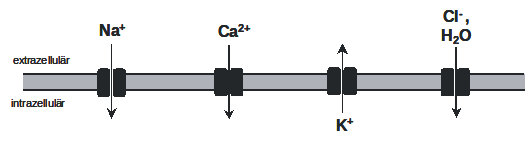
\includegraphics[width=0.4\textwidth]{kanaele.png} 
	\caption{Kanäle der Zellmembran} 
	\label{fig:Kanaele}
\end{figure}
\subsubsection{$Na^+$-Kanäle} (Beispiele)\\
\begin{itemize}
	\item Nicht-Spannungs-abhängig (epitheliale $Na^+$-Kanäle) \textit{Pharmaka:}  Diuretika (z.B.: Amilorid) ENac		                           
	\item Spannungs-abhängige $Na^+$-Kanäle (erregbare Zellen)
		\textit{Pharmaka: } Lokalanästhetika, Klasse-I-Antiarrhythmika, Antiepileptika (z.B.: Lidocain, Phenytoin, Carbamazepin)
\end{itemize}
\subsubsection{$Ca^{2+}$-Kanäle} (Beispiele)
\begin{itemize}
	\item Spannungs-abhängige $Ca^{2+}$-Kanäle \textit{Pharmaka:} $Ca^{2+}$-Kanalblocker (z.B. Dihydropyridine (Nifedipin))
\end{itemize}
\subsubsection{$K^+$-Kanäle} (Beispiele)
\begin{itemize}
	\item Spannungs-abhängige $K^+$-Kanäle \textit{Pharmaka:} Klasse-III-Antiarrhythmika (z.B. Amiodaron, Sotalol)
	\item ATP-regulierte  $K^+$-Kanäle \textit{Pharmaka:} 	Orale Antidiabetika (Sulfonylharnstoffe; z.B. Glibenclamid)
Vasorelaxantien (z.B. Minoxidil)
\end{itemize}
\section{Transporter: Definition und Funktion}
Membranproteine, die selektiv den Transport von Molekülen entlang oder gegen einen elektrochemischen Gradienten erlauben; im Gegensatz zu den Kanälen findet eine Bindung an das Solut sowie eine umfangreiche  des Transporters Konformationsänderung statt; Transportrate: $10^0-10^4 \frac{Molek\ddot{u}le}{Sekunde}$
\subsubsection{Carrier} (primär nicht-aktiver Transporter) \\
	Uniporter, Kotransporter (Symporter), Antiporter (Austauscher)
	Beispiele:
\paragraph{$Na^+$/Neurotransmitter-Kotransporter}
\begin{itemize}
	\item NAT (Noradralin)	\textit{Pharmaka}: Antidepressiva (z.B.: Reboxetin, Desipramin)
	\item SERT (Serotonin)	\textit{Pharmaka}: Antidepressiva (z.B.: Fluoxetin) 
	\item GAT (GABA)	\textit{Pharmaka}: Antiepileptika (z.B.: Tiagabin)
	\item DAT (Dopamin)	\textit{Pharmaka}: Cocain
\end{itemize} 
\paragraph{Kation/Cl--Kotransporter}
\begin{itemize}
	\item NKCC ($Na^+$/$K^+$/2Cl-)	\textit{Pharmaka}: Schleifendiuretika (z.B.: Furosemid)
	\item NCC ($Na^+$/Cl-)		\textit{Pharmaka}: Diuretika (z.B.: Hydrochlorothiazid)
\end{itemize} 
\subsubsection{Pumpen} (aktive, primär ATP-verbrauchende Transporter)\\
\paragraph{Ionenpumpen} (Beispiele)
\begin{itemize}
	\item $Na^+$/$K^+$-ATPase 	\textit{Pharmaka}: Digitalisglykoside (z.B.: Digitoxin)
	\item H+/$K^+$-ATPase		\textit{Pharmaka}: Protonenpumpenhemmer (z.B.: Omeprazol)
\end{itemize}
\paragraph{ABC-Transporter} (ATP-binding cassette; Beispiele)
\begin{itemize}
	\item MDR, MRP		Multidrug resistence gene product Arzneimittelresistenz (z.B. Zytostatika)	
\end{itemize}
\section{Enzyme}
Die meisten Pharmaka, die über Enzyme wirken, hemmen als Substratanaloga das Enzym kompetitiv, reversibel oder irreversibel. Eine Ausnahme stellen z.B. organ. Nitrate dar, die durch Freisetzung von NO die Guanylylcyclase stimulieren.\\
\begin{tabularx}{\textwidth}{X|X|X|X}
Körpereigene Enzyme&Substrat&Produkt&Pharmakon (Beispiel)\\
Oxidoreduktasen&&&\\ \hline
&&&\\
HMG-CoA-Reduktase&HMG-CoA&Mevalonat&Lovastatin, Simvastatin\\
Vit.-K-Reduktase&Vitamin K&Vitamin-K-Hydrochinon&Phenprocoumon\\
$5\alpha$-Reduktase&Testosteron&$5\alpha$-Dihydrotestosteron&Finasterid\\
Cyclooxygenase&Arachidonat&Prostaglandin H2&Acetylsalicylsäure (irrev.); Diclofenac (rev.) u.a.\\
Monoaminoxidase A&Abbau v. Serotonin, Noradrenalin, Dopamin&&Moclobemid (rev.)\\
Monoaminoxydase B&Abbau v. Dopamin, Phenylethylamin u.a.&&Selegilin (irrev.)\\
Xanthinoxydase&Xanthin&Harnsäure&Allopurinol\\
Peroxidase&Tyrosylreste&Iodotyrosylreste&Carbimazol\\
Dihydrofolatreduktase&Dihydrofolat&Tetrahydrofolat&Methotrexat\\
Transferasen&&&\\
Tyrosinkinase&Tyrosinreste&Phosphotyrosinreste&Imatinib, Gefitinib\\
COMT&Catecholgruppe&Methoxycatechol&Entacapon\\
GABA Transaminase&GABA&Succinatsemialdehyd&Vigabatrin\\
Hydrolasen&&&\\
Phosphodiesterase&cAMP, cGMP&AMP, GMP&Theophyllin, Sildenafil\\
Acetylcholinesterase&Acetylcholin&Cholin, Acetat&Tacrin, Neostigmin, Sarin(irrev.)\\
Calcineurin (Phosphatase)&P-Ser/Thr/Tyr&Ser/Thr/Tyr&Ciclosporin,Tacrolimus\\
$\alpha$-Glucosidase&Disaccharid&Monosaccharid&Acarbose\\
Renin&Angiotensinogen&Angiotensin I&Aliskiren\\
ACE/Kininase II&Angiotensin I&Angiotensin II&Captopril, Lisinopril\\
Thrombin (Faktor IIa)&Fibrinogen&Fibrin&Hirudin, Dabigatrann\\
Enkephalinase&Enkephalin&&Racecadotril\\
Dipeptidylpeptidase IV&GLP-1(7-36)&GLP-1(9-36)&Sitagliptin, Vildagliptin\\
Lipase&Triacylglycerine&Monoacylglycerin, FS&Orlistat\\
Lyasen&&&\\
Guanylyl cyclase&GTP&cGMP&Glyceroltrinitrat, Molsidomin\\
Dopamin-decarboxylase&L-Dopa&Dopamin&Benserazid, Carbidopa\\
\end{tabularx}
\begin{tabularx}{\textwidth}{X|X}
Mikrobielle Enzyme&Pharmakon (Beispiel)\\ \hline \\
Bakterien&\\
Peptidoglykansynthetasen&$\beta$-Laktame\\
Dihydrofolat-Reduktase&Trimethoprim\\
Dihydropteroat Synthase&Sulfonamide\\
bakt. Topoisomerase II&Gyrasehemmer\\
Pilze&\\  
Lanosterol C14 Demethylase&Azole\\
Squalenepoxidase&Allylamine\\
Protozoen&\\
Dihydrofolat-Reduktase&Pyrimethamin\\
Viren&\\
HIV Reverse Transkriptase&Zidovudin, Didanosid\\
HIV Protease&Saquinavir\\
Neuraminidase&Zanamivir\\
\end{tabularx}
\section{Rezeptor: Definition und Funktion}
\begin{enumerate}
	\item Erkennen (hohe Spezifität) und reversibles Binden (hohe Affinität) des Wirkstoffes (physiol. Ligand oder Pharmakon)
	\item Bindung löst Signalweiterleitungsfunktion aus
\end{enumerate}
\section{Rezeptortypen}
\begin{itemize}
	\item membranär
	\begin{itemize}
		\item G-Protein-gekoppelte Rezeptoren
		\item Liganden-gesteuerte Ionenkanäle
		\item Liganden-regulierte Enzyme
			multimere Rezeptoren 
	\end{itemize}
	\item zytosolisch/nukleär
	\begin{itemize}
		\item nukleäre Rezeptoren
	\end{itemize}
\end{itemize}
\section{G-Protein-gekoppelte Rezeptoren (GPCR)}
ca. 1500 Säugergene für G-Protein-gekoppelte Rezeptoren, davon ca. 1000 olfaktorische, gustatorische und Pheromon-Rezeptoren sowie ca. 500 Rezeptoren für Hormone, Neurotransmitter u.a.
\subsection{Aktivierungs-/Inaktivierungs-Zyklus}
\section{G-Protein vermittelte Signalwege (ubiquitär)}
\subsection{Gs-gekoppelte Rezeptoren}
$\rightarrow$ Adenylylcyclase$\uparrow$ $\rightarrow$ cAMP$\uparrow$ $\rightarrow$ PKA$\uparrow$ $\rightarrow$ Proteinphosphorylierung
\subsubsection{Beispiele}
$\beta_{1,2}$-adrenerg	, Histamin $H_2$,Dopamin $D_1,D_5$, Prostacyclin IP, Adenosin $A_2$, Vasopressin $V_2$
\subsection{Gi/o-gekoppelte Rezeptoren}
$\rightarrow$Adenylylcyclase $\downarrow$ $\rightarrow$ cAMP$\downarrow$
$\rightarrow$ Spannungsabh. $Ca^{2+}$-Kanal $\downarrow$ 
$\rightarrow$ $K^+$-Kanal (GIRK) $\uparrow$
$\rightarrow$ Erregbarkeit $\downarrow$
\subsubsection{Beispiele}Opioide ($\mu,\delta,\kappa$),GABAB,Cannabinoide $CB_{1,2}$	Dopamin $D_{2-4}$, mGluR2-4,6-8, $\alpha_24$-adrenerg, muskarinerg M$_{2,4}$,Adenosin A$_1$, Somatostatin Sst$_{1-5}$, 5-HT$_1$
Chemokine CCR1-10; CXCR1-5 \\ \\
\scriptsize
\begin{tabularx}{\textwidth}{XXXX}
Physiol. Ligand&Rezeptor&G-Protein(e)&Pharmaka (Beispiele)\\
Aminosäuren&&&\\
Glutamat&mGluR1,5;2-4,6-8&$G_{q/11}; G_{i/o}$&DHPG (1/5-Ag, experimentell)\\
GABA&$GABA_{B1} / GABA_{B2}$&$G_{i/o}$&Baclofen (Ag)\\
Biogene Amine&&&\\
Acetylcholin&$M_1, M_3, M_5; M_2, M_4$&$G_{q/11}; G_{i/o}$&Atropin (Ant); Carbachol (Ag)\\
(Nor)Adrenalin& $\alpha_{1A}, \alpha_{1B}, \alpha_{1D}, \alpha_{2A}, \alpha_{2B}, \alpha_{2C}, $&$G_{q/11}; G_{i/o}, G_S$&Phenylephrin (Ag); Prazosin (Ant)  Clonidin (Ag); Yohimbin (Ant) Isopropanol (Ag); Propranolol (Ant)\\
$\beta_1, \beta_2, \beta_3$&&\\
Dopamin&$D_1,D_5; D_2,D_3,D_4$& $G_{S}; G_{i/o}$&Bromocriptin/Haloperidol($D_{2-4}$-Ag/Ant)\\
Histamin&$H_1; H_2; H_3,H_4$&$G_{q/11}; G_{i/o}, G_S$&Loratadin (H1-Ant); Ranitidin (H2-Ant)\\
Serotonin&5-$HT_{1A/B/D/E/F}$5-$HT_{2A/B/C}; $5-$HT_{4/6/7}$&$G_{q/11}; G_{i/o}, G_S$& Sumatriptan(1B/D-Ag);Buspiron(1A-Ag), Risperidon (2A-Ant); Cisaprid (4-Ag)\\
Melatonin&$MT_1,MT_2$&$G_{i/o}$&Ramelteon (Ag)\\
Trace Amines&$TA_1, TA_2$&$G_S$&\\
Ionen&&&\\
Calcium&CaSR&$G_{q/11}; G_{i/o}$&Cinacalcet (Modul.)\\
Nukleotide / Nukleoside&&&\\
Adenosin&$A_1,A_3; A_{2A}, A_{2B}$&$G_{i/o}, G_S$&Theophyllin, Coffein (Ant)\\
ADP&$P2Y_{12}, P2Y_{13}$&$G_{i/o}$&Clopidogrel ($P2Y_{12}$-Ant)\\
Lipide&&&\\
Endocannabinoide&$CB_1, CB_2$&$G_{i/o}$&$\Delta$9-THC (Ag); Rimonabant (CB1-Ant)\\
$LTC_4, LTD_4$&$CysLT1, CysLT2$&$G_{q/11}$&Montelukast (Ant)\\
Lysophospholipide&$LPA_{1-5}, S1P_{1-5}$&$G_{q/11},G_{12/13}, G_{i/o}$&Fingolimod (FTY720; S1P-Ag.)\\
Prostacyclin ($PGI_2$)&IP&$G_s$&Iloprost (Ag)\\
Prostaglandin $E_2$&$EP_1; EP_2; EP_4; EP_3$&$G_{q/11}; G_s; G_{q/11}, G_i$&Misoprostol (Ag)\\
Peptide / Proteine&&&\\
Angiotensin II&$AT_1; AT_2$&$G_{q/11}, G_{12/13}, G_{i/o}; ?$&Losartan (AT1-Ant)\\
Bradykinin&$B_1, B_2$&$G_{q/11}$&Icatibant($B_2$-Ant; experim.)\\
CGRP&CL+RAMP1&$G_{q/11}. G_S$&BIBN 4096 BS (Ant, exp.)\\
Chemokine&CCR1-10;CXCR1-5&$G_{i/o}$&Maraviroc (CCR5-Antag.)\\
Cholecyctokinin&$CCK_1, CCK_2$&$G_{q/11}. G_S$&\\
Komplem. C3a / C5a&C3a; C5a&$G_{i/o}$&\\
Endothelin- 1, -2, -3&$ET_A; ET_B$&$G_{q/11}, G_{12/13}, G_s$&Bosentan (ETA/B-Ant), Darusentan (ETA-Ant)\\
Galanil&GAL1-3&$G_{q/11}, G_{i/o}$&\\
Glucagon-like pept.&GLP1-3&$G_S$&Exenatid (Ag)\\
Glykoproteinhorm.&TSH, LH, FSH&$G_s$&\\
Melanocortine&MC1,3,4,5&$G_S$&\\
Glukagon&Glukagon&$G_S$&\\
Gonadoliberin&GnRH&$G_{q/11}$&Buserelin (Ag)\\
Motilin&GPR38&$G_{q/11}$&Erythromycin (Ag)\\
Opioide&$\gamma, \kappa, \mu$, ORL1&$G_{i/o}$&Morphin (Ag), Naloxon (Ant)\\
Orexin A/B&OXYD, OX2&$G_s, G_{q/11}$&\\
Oxytocin&OT&$G_{q/11}, G_{i/o}$&Atosiban (Ant, experimentell)\\
PTH&PTH/PTHrP&$G_s, G_{q/11}$&Teriparatid (Ag)\\
Sekretin&Secretin&$G_s$&\\
Somatostatin&$SST_{1-5}$&$G_{i/o}$&Octreotid (Ag)\\
Substance P&$NK_1$&$G_{q/11}$&Aprepitant (Ant)\\
Urotensin II&UT-II (GPR14)&$G_{q/11}$&\\
VIP, PACAP&$VPAC_{1,2}, PAC_1$&$G_s$&\\
Vasopressin&$V_{1a}, V_{1b}; V_2$&$G_{q/11}; G_s$&Desmopressin ($V_2$-Ag), Terlipressin ($V_1$-Ag)\\
Proteasen (der durch proteolyt. Spaltung gebildete “neue” N-Terminus fungiert als interner Ligand)&&&\\
Thrombin u.a.&PAR-1/2/4&$G_{q/11}, G_{12/13}, G{i/o}$&\\
Trypsin u.a.&PAR-2&$G_{q/11}$&\\
“orphan”-Rezeptoren (physiologischer Ligand bisher unbekannt)\\
?&GRP109A (HM74a)&$G_i$&Nikotinsäure (Ag)\\
\end{tabularx}
\normalsize
\section{Liganden-gesteuerte Ionenkanäle}
\begin{tabularx}{\textwidth}{XXXX}
Rezeptor&Ligand&Kanaltyp&Pharmaka(Beispiele)\\
Pentamere&&&\\
nikotinisch&Acetylcholin&$Na^+/ K^+$&Curare/Muskelrelaxantien (Ant)\\
$5-HT_3$&Serotonin&$Na^+/ K^+$&Ondansetron (Ant; Antiemetika)\\
$GABA_A$&$GABA_A$&$Cl^-$&Benzodiazepine (Modul.)\\
Glyzin-R.&Glyzin-R.&$Cl^-$&Strychnin (Ant)\\
Tetramere&&&\\
NMDA&Glutamat&$Na^+/ K^+/ (Ca^{2+})$&Phencyclidin (Ant), Memantin (Modul.)\\
AMPA&“&$Na^+/ K^+$&\\
Kainat&“&$Na^+/K^+$&\\
Trimere&&&\\
ATP&P2X&$Na^+/ K^+/ (Ca^{2+})$&\\
\end{tabularx}
\section{Liganden-regulierte Enzyme}
\subsection{Rezeptoren mit Tyrosinkinase-Aktivität (Beispiel: Insulin-Rezeptor)}
BILD!
\begin{itemize}
	\item Insulin-Rezeptor Familie:  Insulin, Insulin-like growth factor (IGF-1) etc.
	\item Pharmaka: verschiedene Insuline
	\item ErbB Rezeptor Familie: Epidermal growth factor (EGF), ErbB1-4 etc.
	\item Pharmaka: Trastuzumab (Antikörper gegen ErbB2/Her2)
	\item Gefitinib, Erlotinib (Tyrosinkinasehemmer mit Selekt. für ErbB1)
	\item Cetuximab (Antikörper gegen ErbB1)
	\item Platelet-derived growth factor (PDGF)- Rezeptor Familie: PDGF, CSF, SCF
	\item Pharmaka: Imatinib (Tyrosinkinasehemmer mit Selekt. v.a. für BCR-ABL) 
	\item Vascular endothelial growth factor (VEGF)-Rezeptor Familie : VEGF
	\item Pharmaka: Bevacizumab (Antikörper gegen VEGF)
	\item Fibroblast growth factor (FGF)-Rezeptor Familie: FGF 
	\item Nerve growth factor (NGF)-Rezeptor Familie: NGF, Neurotrophins etc.
	\item Hepatocyte growth factor (HGF): HGF 
	\item Eph family receptors: Ephs, Ephrins;   Axl; Tie; etc..
\end{itemize}
\section{nukleäre Rezeptoren}
\begin{tabularx}{\textwidth}{XXX}
Ligand&Rezeptor A/B&Pharmaka (Beispiele)\\
Östrogen&ER/ER&Ethinylestradiol (Ag); Tamoxifen(Ag/Ant); Clomiphen (pAg)\\
Progesteron&PR/PR&Norethisteron (Ag), Mifepriston (Ant)\\
Androgen&AR/AR&Nandrolon (Ag), Flutamid (Ant)\\
Aldosteron&MR/MR&Spironolacton (Ant); Fludrocortison (Ag)\\
Glukokortikoide&GR/GR&Dexamethason (Ag)\\
Retinsäure&RAR/RXR&Acitretin (Ag)\\		
Schilddrüsenhormon&TR/RXR&T$_3$ (Ag)\\
Vitamin D&VDR/RXR&Tacalcitol (Ag)\\
Gallensäuren&FXR/RXR&\\
Oxysterole&LXR/RXR&\\
Xenobiotika&Ah-Rezeptor/ARNT&Dioxin (Ag)\\
Xenobiotika&CAR / RXR&Barbiturate (Ag)\\
Xenobiotika&PXR bzw. SXR/RXR&Rifampicin (Ag) u.a.\\	
Fettsäuren&PPAR$\alpha$ / RXR&Fibrate (Ag)\\
Fettsäuren&PPAR$\gamma$ / RXR&Thiazolidindione (Ag)\\
\end{tabularx}
\section{Pharmakon-Rezeptor-Interaktion}
\begin{figure}[h]
\begin{reaction}
	\ce{P + R <-->[{k_1}][{k_2}] PR}
\end{reaction}	
\begin{reaction}
	\ce{\frac{[P] * [R]}{[PR]}=\frac{k_2}{k_1}=K_D}
\end{reaction}
\caption{Pharmakon-Rezeptor-Interaktion:\textit{k1}: Geschwindigkeitskonstante der Assoziation;
\textit{k2}: Geschwindigkeitskonstante der Dissoziation 
im Äquilibrium gilt gemäß Massenwirkungsgesetz:
\textit{KD}: Äquilibrium-Dissoziations-Konstante
       Maß für die Affinität
KD der meisten physiologischen Rezeptoren im Bereich von: 10-9 - 10-6 M}
\end{figure}
\section{Wirkungsauslösung}
\begin{figure}
\begin{reaction}
	\ce{P + R <-->[{k_1}][{k_2}] PR ->[{proportional}] Effekt}
\end{reaction}
\caption{Wirkungsauslösung: Der Effekt ist proportional der Rezeptor-Besetzung}
\end{figure}

\subsubsection{Intrinsische Aktivität 
(Wirksamkeit, „efficacy“)}Maß für die maximale Wirkung 
eines Pharmakons
\subsubsection{Konzentrations-
Wirkungs-Beziehung:}$EC_{50}$:effektive Konzentration 50\% $\neq K_D$
\section{Wirksamkeit/Potenz}
\subsubsection{Potenz:}Maß für die 
Konzentration einer Substanz, 
die zur Erreichung der halb-
maximalen Wirkung 
notwendig ist
\subsubsection{Wirksamkeit:}Maß für 
die maximal erreichbare 
Wirkung
\section{Agonismus}
\begin{itemize}
 \item unbesetzter Rezeptor hat basale Aktivität
	\item Agonist: Affinität zu Rezeptor + intrinsische Aktivität 
		\begin{itemize}
		\item	volle/partielle Wirksamkeit $\rightarrow$ voller/partieller Agonismus
		\item negativ intrinsische Aktivität $\rightarrow$ inverser Agonismus
		\end{itemize}	
	\item Antagonist/Blocker: Affinität zu Rezeptor, keine intrinsische Aktivität	
\end{itemize}
\section{Antagonismus}
\subsubsection{Agonist:}Affinität zum Rezeptor
+ intrinsische Aktivität
\subsubsection{Antagonist:} Affinität zum Rezeptor, 
keine intrinsische Aktivität
\subsubsection{kompetitiver Antagonismus} Antagonist konkurriert mit Agonist um 
Bindungsstelle $\rightarrow$ Parallelverschiebung der DWK
\subsubsection{nichtkompetitiver Antagonismus}
\begin{itemize}
	\item keine Kompetition mit Agonist, eher selten
	\item Beeinflussung der Rezeptor-Effektor-Kopplung
	\item Wirkung kann durch hohe Agonist-Konzentrationen nicht aufgehoben werden
	\item Maximaleffekt des Agonisten	verringert
\end{itemize}
\section{Toleranzphänomene}
\subsection{Toleranz:} abnehmende Wirkung nach wiederholter Gabe bei gleicher Dosis
\subsubsection{pharmakokinetische Toleranz} z.B. Metabolisation $\uparrow$ (Barbiturate, Äthanol)
\subsubsection{pharmakodynamische Toleranz} z.B.: Rezeptorzahl $\downarrow$ ($\beta$-Adrenozeptor-Agonisten)
\subsection{Tachyphylaxie}
sehr rasche Toleranzentwicklung (Minuten bis Stunden)
\begin{itemize}
	\item indirekte Sympathomimetika
	\item (organische Nitrate; Stunden bis Tage)
\end{itemize}
\section{Unerwünschte Wirkungen von Pharmaka}
\subsubsection{Hauptwirkung} therapeutisch erwünschte Wirkung
\subsubsection{Nebenwirkung} jede Reaktion außerhalb der Hauptwirkung
\subsubsection{Unerwünschte Wirkung} jede unerwünschte Reaktion, die auf die Verordnung eines Arzneimittels ursächlich zurückgeführt werden kann
\begin{equation}
erw\ddot{u}nschte\:therapeutische\:Wirkung\:(Hauptwirkung) \longleftrightarrow  unerw\ddot{u}unschte\:Wirkung\:(Nebenwirkung)
\end{equation}

\subsection{Häufigkeit unerwünschter Arzneimittelwirkungen}
2 - 5\% in der Praxis 		\\
6 - 20\% in der Klinik\\
ca. 5\% der Klinikaufnahmenerfolgen wegen unerw. Arzneimittelwirkungen\\
\glqq Alle Dinge sind Gift und nichts ist ohn’ Gift; allein die Dosis macht, daß ein Ding kein Gift ist.Paracelsus\grqq
\subsection{Unerwünschte Wirkungen im Rahmen des
pharmakodynamischen Wirkprofils}
treten bei jedem Patienten dosisabhängig und spezifisch auf: \glqq Die Dosis macht das Gift\grqq
\begin{itemize}
	\item bei therapeutischer Dosierung   z.B.: Zytostatika
	\item erst bei Überdosierung: Pharmaka mit geringer therapeutischer Breite (Beispiele):	Digitalisglykoside, Cumarin-Derivate, Lithium, Theophyllin
\end{itemize}
\subsection{Ursachen dosisabhängiger unerwünschter Arzneimittelwirkungen}
\subsubsection{Absolute Überdosierung} durch Verordnungs- oder Einnahmefehler
\subsubsection{Relative Überdosierung} durch verminderte Elimination (Metabolisierung/Ausscheidung) oder verstärkte Wirkung
\subsection{Arzneimittel-unabhängige Faktoren, die zu einer relativen Überdosierung führen}
\begin{itemize}
	\item Alter des Patienten: 
	\begin{itemize}
		\item Kinder: Besonderh. der Pharmakokinetik (Verteilungsvolumen$\uparrow$; hepat. Metabol. und renale Ausscheidung: $\downarrow$ bei Früh- /Neugeborenen; $\uparrow$ ab 1-2 Monaten) Nur bei Kindern auftretende unerwünschte Wirkungen	z.B.: Tetracycline $\rightarrow$ Gelbfärbung der Zähne, Kariesanfälligkeit;	Acetylsalicylsäure $\rightarrow$ Reye-Syndrom; Chloramphenicol $\rightarrow$ Grey-Syndrom
		\item ältere Menschen
		\begin{itemize}
			\item Polymorbidität, Compliance
			\item Pharmakokinetik (hepatische Metabolisierung $\downarrow$; renale Elimination $\downarrow$)
		\end{itemize}
	\end{itemize}	 
	\item Einfluss der Krankheit
	\begin{itemize}
		\item auf Pharmakokinetik (z.B.: Metabolisierungs- und Ausscheidungsstörungen 
		bei Leber- und Nierenerkrankungen)
		\item auf Pharmakodynamik (z.B.: Hypokaliämie $\rightarrow$ verstärkte Digitaliswirkung)
	\end{itemize}
	\item Schwangerschaft und Stillzeit
	\begin{itemize}
		\item Unerw: Wirkungen in der Schwangerschaft meist Phasen-spezifisch
		\item Blastogenese  bei Schädigung $\rightarrow$ Abstoßung
		\item Embryogenese/Organogenese (Tag 15 - Tag 60) hohe Gefährdung durch teratogene Substanzen ! z.B.: Thalidomid $\rightarrow$ Phokomelien, Lithium $\rightarrow$ Herzmißbildungen, Alkohol $\rightarrow$ Entwicklungsverzögerung, Gesichtsmißbildungen,	Phenytoin $\rightarrow$ Gaumenspalten
		\item Fetalphase (Histogenese/funktionelle Reifung; 3. Monat - Geburt) keine teratogene Gefährdung, aber selektive unerwünschte Wirkungen v.a. auf Funktion und Wachstum des Fetus z.B.: 	ACE- Hemmer: gegenüber der Mutter gesteigerte Empfindlichkeit des Fetus $\rightarrow$ RR $\downarrow$ $\rightarrow$ Nierenfunktion $\downarrow$ $\rightarrow$ Anurie $\rightarrow$ Fruchtwassermangel; Tetrazykline: Einlagerung als $Ca^{2+}$-Komplex in Zahnschmelz und Knochen $\rightarrow$ Gelbfärbung der Zähne, evtl. Knochenschädigungen; Stillzeit: Im Gegensatz zur Schwangerschaft geringere Gefahr unerwünschter Wirkungen auf Kind
	\end{itemize}
	\item Pharmakogenetische Faktoren
	\begin{itemize}
		\item Pharmakokinetik	z.B.: Polymorphismen Arzneimittel-metabolisierender Enzyme
	 	\item Pharmakodynamik z.B.: Polymorphismen von pharmakologischen Zielstrukturen
	\end{itemize}
\end{itemize}
\subsection{Unerwünschte Wirkungen durch Arzneimittelinteraktionen}
Häufigkeit steigt exponentiell mit Anzahl der verabreichten Pharmaka
Auftreten unerw. Wirkungen, aber auch Wirkungsabschwächung
\subsubsection{Beispiele}\mbox{} \\
\begin{tabularx}{\textwidth}{XXX}
Pharmakokinetisch&&\\
Resorption&&Effekte\\                                                                       
$Ca^{2+}, Mg^{2+}, Al^{2+}, Fe^{2+},$ &+ Tetracycline & Tetracyclinresorption $\downarrow$\\
Colestyramin&+Digitalisglyk., Thyroxin u.a.&Resorption $\downarrow$\\
Metabolismus&&\\
CYP3A4 Induktion&&\\
Johanniskraut, Rifampicin&+ Ciclosporin&Transplantatabstoßung\\
Phenytoin, Carbamazepin&+ Ethinylestradiol&“Pillenversager”\\
HIV-Protease Hemmer&&Wirkverlust der antiviralen Therapie\\
CYP3A4 Hemmung&&\\
Azol-Antimykotika,&+ Statine&Statin-Abbau $\downarrow$ $\rightarrow$ Myopathierisiko $\uparrow$\\
HIV-Proteasehemmer,& + Ciclosporin& Nephrotoxizität $\uparrow$\\
Makrolide, Grapefruitsaft& + Cisaprid, Terfenadin& Long-QT-S., Torsade de Pointes\\
CYP2C9 Induktion&&\\
Rifampicin, Phenytoin&+ Cumarine&Thromboserisiko $\uparrow$\\
CYP2D6 Hemmung&&\\
Fluoxetin, Paroxetin&+ Trizykl. Antidepressiva&Kardiale Effekte\\
Ausscheidung&&\\
Diuretika&+ Lithium&Lithiumausscheidung $\downarrow$\\
ASS&+ Methotrexat&Methotrexattoxizität $\uparrow$\\
Pharmakodynamisch&&\\
additive Effekte&&\\
Fibrate&+ Statine&Myopathierisiko $\uparrow$\\
$\beta$-Blocker&+ Verapamil/Diltazem&Bradykardie, AV-Block, Herzinsuff.\\
Aminoglykoside&+ Schleifendiuretika&Oto-, Nephro-Toxizität $\uparrow$\\
PDE5-Hemmer&+ organ. Nitrate&Schwere Hypotension\\
MAOA-Hemmer&+ SSRI (z.B.: Fluoxetin)&Serotoninsyndrom\\
ASS, Clopidogrel&+ Cumarinderivate&Blutungsneigung (v.a. Magen/Darm) $\uparrow$\\
$K^+$-sparende Diuretika&+ ACE-Hemmer/AT1-Blocker&Hyperkaliämiegefahr\\
Benzodiazepine&+ Ethanol&Sedation$\Uparrow$\\
Antagonistischer Effekt&&\\
NSAIDs (z.B. Ibuprofen, Indomethacin)&+ Antihypertensiva(v.a. Diuretika)&Aufhebung der antihypertensiven Wirkung\\
$\beta$-Blocker&+ $\beta_2$Agonisten&Antiasthmat. Effekt $\downarrow$\\
L-Dopa&+ klass. Neuroleptika&gegenseit. Abschwächung der Effekte\\
Ibuprofen&+ ASS&Thrombozytenfunktionshemmung $\downarrow$\\
\end{tabularx}
\subsection{Unerw.Wirkungen außerhalb des pharmakodynam. Wirkprofils}
dosisunabhängig, nicht Arzneistoff-spezifisch, meist allergisch\\
\subsubsection{Arzneimittelallergie}: Arzneistoff / Metabolit bindet (als Hapten) an körpereigenes Makromolekül $\rightarrow$ Bildung eines Vollantigens $\rightarrow$ Bildung von Antikörpern oder sensibilisierten T-Lymphozyten $\rightarrow$ allergische Reaktion nach Reexposition
\subsubsection{Pseudoallergische Reaktion}: meist dosisabhängige, unspezif. Aktivierung immunologischer Prozesse, z.B. Freisetzung v. Mediatoren aus Mastzellen 
\chapter{Cholinerges System}
\section{cholinerge und adrenerge Übertragung im peripheren efferenten Nervensystem}
\subsection{Eigenschaften des somatomotor. und autonomen Systems}
\begin{tabularx}{\textwidth}{XXX}
&somatomotor. System&autonomes System\\
distale Synapse&Vorderhorn&	Ganglion\\
Plexusbildung&nein&ja (v.a. Sympathikus)\\
Verzweigung&ja (motor. Einheit)&ja (Symp.$>$Parasymp.)\\
Myelinisierung&Nerven myelinisiert&postganglionär nicht myelinisiert\\
\end{tabularx}
\section{Acetylcholin}
\subsection{Cholinerge Synapse}
Depolarisation $\rightarrow$ $Ca^{2+}$-Einstrom $\rightarrow$ 	Freisetzung von Ach aus Vesikeln in den synapt. Spalt $\rightarrow$ Bindung von Ach an postsynapt. Rezeptor $\rightarrow$ Inaktivierung von Ach durch Acetylcholinesterase (260 kDa, $\alpha$2,$\beta$2-Struktur, ca. 20.000/s)
\subsection{Acetylcholinesterase}
\subsubsection{motorische Endplatte}
3 x 4 enzymatische Untereinheiten über Kollagenanker an Basalmembran des synaptischen Spalts verankert extrem hohe Umsatzrate (ca. 20.000 Ach-Moleküle/s)
\subsubsection{ZNS}
1 x 4 enzymatische Untereinheiten, über Lipidrest in Plasmamembran verankert
\subsubsection{sezernierte Form} 
1 x 4 enzymatische Untereinheiten, hydrophil
Acetylcholin-spezifische Form: u.a. Liquor
unspez. Cholinesterase (Pseudocholinesterase, Butyrylcholinesterase): v.a. in der Leber synthetisiert, hohe Aktivität im Plasma
\section{Pharmakologische Beeinflussung cholinerger Systeme}
\begin{itemize}
	\item Nikotinischer Ach-Rezeptor (Agonisten/Antagonisten)
	\item Muskarinischer Ach-Rezeptor (Agonisten) $\rightarrow$ Direkte Parasympathomimetika
 	\item Muskarinischer Ach-Rezeptor (Antagonisten) 
   $\rightarrow$ Direkte Parasympatholytika
	\item Acetylcholinesterase-Hemmer 
   $\rightarrow$ Indirekte Parasympathomimetika
\end{itemize}
\subsection{Cholinerge Rezeptoren}
\subsubsection{muskarinisch}
G-Protein-gekoppelte Rezeptoren\mbox{} \\
\begin{tabularx}{\textwidth}{XXXX}
Rezeptorsubtyp&Hauptlokalisation&zellulärer Effekt&Effektorsystem\\
$M_1$&neuronal ZNS&Exzitation &\\
&auton. Ganglien&Magensaftsekretion $\uparrow$&PLC$\uparrow$ ($G_{q/11}$)\\
&(v.a. enteral)&M.-D.-Motilität $\uparrow$&\\
$M_2$&kardial Sinusknoten&diastol. Depolar.$\downarrow$ $\Rightarrow$ HF $\downarrow$ &$K^+$-Kanal$\uparrow$\\
&AV-Knoten&Fortleitung $\downarrow$&$Ca^{2+}$-Kanal $\downarrow$\\ 
&Atrium (Ventrikel)&Kontraktionskraft $\downarrow$&A-cyclase $\downarrow$\\
&präsynaptisch&Transmitterfreisetzung $\downarrow$&($G_{i/o}$)\\
$M_3$&exokrine Drüsen (Pankreas, Parotis)&Sekretion $\uparrow$&\\
&glatte Muskulatur(Bronch., Darm, Harnbl.)&Kontraktion $\uparrow$&PLC $\uparrow$ ($G_{q/11}$)\\
&vaskuläres Endothel&Vasodilatation (NO-Freisetz.)&\\
&Auge (Ziliarmuskel,M. constr. pupillae)&Kontraktion (Nahakkomod.),  Kontraktion (Miosis)&\\
$M_4$&ZNS&?&wie $M_2$\\
$M_5$&weit verbreitet (low level)&?&PLC $\uparrow$ ($G_{q/11}$)\\
\end{tabularx}
\subsubsection{nikotinisch}	
ionotrope Rezeptoren, Pentamere, 
2 $\alpha$-Untereinheiten ($\alpha$2-10
3 $\beta$-Untereinheiten ($\beta$2-4)
$\alpha$-Untereinheit bindet Ach
Rezeptor bildet $Na^+/K^+$-Kanal, 
der d. Bindung von Ach geöffnet wird 
$\rightarrow$ $Na^+$-Einstrom $\rightarrow$ Depolarisation 
 
$N_M$ 	(muskulärer Typ)
($\alpha$1)$_2$,$\beta$1,$\delta$,$\epsilon$ (embryonal/denerv. Muskel:$\gamma$ statt $\epsilon$)
neuromuskuläre Endplatte der Skelettmuskulatur, vermittelt Kontraktion	
$N_N$ 	(neuronaler Typ)
($\alpha$4)$_2$/($\beta$2)$_3$ 	häufig im ZNS, (v.a. $K^+/Na^+$ permeabel)
($\alpha$7)$_5$ 	häufig im ZNS, (auch $Ca^{2+}$ permeabel)
($\alpha$3)$_2$/($\beta$4)$_3$ Ganglion-Typ $\rightarrow$ Depolarisation/Weiterleitung; 
NN-Mark $\rightarrow$ Sekretion von Katecholaminen
\subsection{Agonisten / Antagonisten des nikotinischen Ach-Rezeptor}
\subsubsection{Nikotin}(agonistische Wirkung v.a. auf neuronalen Rezeptor ($N_N$) \\
\paragraph{Pharmakokinetik}
\begin{itemize}
	\item rasche Aufnahme über Mundschleimhaut oder Lunge (je nach pH-Wert)
    \item gute Verteilung (insb. ZNS) der nicht-ionisierten Form; Plasma-HWZ: 2-3 h
    \item 80\% hepat. metabolisiert zu Cotinin
\end{itemize}
\paragraph{Pharmakodynamik}
 niedrige Dosis: Ganglien  erregend $\rightarrow$ Adrenalinfreisetzung aus NNM, RR$\uparrow$, hohe Dosis: Ganglien blockierend (Depol.) + zentrale Effekte
$\rightarrow$ komplexe Effekte: Durchfall, Magensaftproduktion $\uparrow$, RR$	\upharpoonleft\downharpoonright$ , HF$	\upharpoonleft\downharpoonright$, Speichelsekretion $\uparrow$ , Übelkeit, Tremor; Krämpfe, Atemlähmung Sucht-erzeugende Wirkung durch Aktivierung des „reward pathways Toxizität: 50 mg tödlich (1 Zigarette $\simeq$ 10 mg)
\subsubsection{Cytisin / Vareniclin}(partieller Agonismus an ($\alpha$4)2($\beta$2)3 Rezeptoren Cytisin z.B. im Goldregen vorkommend, 3-4 Früchte für Kleinkinder tödlich Abkömmling Vareniclin als Raucherentwöhnungsmittel 3/07 zugelassen.
\subsubsection{Muskelrelaxantien}(Wirkung v.a. auf muskulären Rezeptor ($N_M$))
\begin{itemize}
	\item nicht-depolarisierende Muskelrelaxantien kompetitive Antagonisten am muskulären nikotinischen Ach-Rezeptor
	\item depolarisierende Muskelrelaxantien Agonisten am muskulären nikotinischen Ach-Rezeptor
\end{itemize}
\paragraph{Wirkung} Motorische Lähmung, keine Bewusstseinsbeeinflussung
äußere Augenmuskeln $\rightarrow$ Zunge $\rightarrow$ Finger $\rightarrow$ Nacken $\rightarrow$ Stamm $\rightarrow$ Extremitäten $\rightarrow$ Atemmuskulatur
\paragraph{Einsatz} V.a. Narkose
\paragraph{Pharmakokinetik} Quarternären Stickstoff $\rightarrow$ schlechte Resorption nach oraler Gabe $\rightarrow$ keine ZNS-Gängigkeit
\subsection{nicht-depolarisierende Muskelrelaxantien}
\textit{Tubocurarin}: Wirkdauer 60-80 min; zusätzliche Wirkungen: Histaminfreisetzung aus Mastzellen Ganglienblockade $\rightarrow$ RR$\downarrow$;  obsolet.
\begin{tabularx}{\textwidth}{XXXX}
&Potenz (im Vergl. zu Tubocurarin)&Wirkdauer&Wirkbeginn\\
Benzylisochinoline&&&\\
Atracurium&ca. 2x&20-35 min&2-4 min\\
Mivacurium&ca. 3x&15-25 min&2-4 min\\
Steroidderivate&&&\\
Pancuronium&ca. 5x&60-120 min&4-6 min\\
Vecuronium&ca. 5x&45-90 min&2-4 min\\
Rocuronium&ca. 0,5x&35-70 min&1-2 min!\\
\end{tabularx}
\paragraph{Elimination}spontan (Atracurium); unspez. Esterasen (Atracurium, Mivacurium) renal/hepatisch: Steroidderivate
\paragraph{Antidot} Acetylcholinesterase-Hemmer
\subsection{depolarisiernde Muskelrelaxantien}
\subsubsection{Suxamethonium, Succinylcholin}
\paragraph{Wirkung} Agonismus am Rezeptor, langsamer Abbau persistierende Depolarisation $\rightarrow$ Inaktiv. spannungsabh. Na$^+$-Kanälen $\rightarrow$ Sarcolemm elektrisch unerregbar; kein Antagonismus durch Ach-esterase-Hemmer! Wirkdauer 5-10 min, Abbau d. Esterspaltung (unspez. Cholinesterasen)
\paragraph{Einsatz}  nur noch selten eingesetzt (kurzdauernde Eingriffe)
\paragraph{unerwünschte Wirkungen} protrahierte Apnoe (hereditärer Cholinesterase-Mangel); Muskelkater-ähnliche Symptome; Hyperkaliämie;  maligne Hyperthermie
\section{Agonisten / Antagonisten muskarinischer Rezeptoren
antimuskarinerge Substanzen / Parasympatholytika}
\subsection{Belladonna-Alkaloide}
\begin{itemize}
	\item Atropin tertiäres Amin $\rightarrow$ gute Resorption, ZNS-gängig $\rightarrow$ Exzitation
	\item Scopolamin tertiäres Amin $\rightarrow$ gute Resorption, ZNS-gängig
$\rightarrow$ Dämpfung; i.G. zu Atropin stärker mydriatisch, sekretionshemmend, schwächer spasmolyt., kardial wirks.
\end{itemize}
\paragraph{Wirkung}
\begin{itemize}
	\item Auge:	Mydriasis, Akkomodationslähmung (8–12 d), intraokularen Drucks $\uparrow$
	\item Herz:	Tachykardie, AV-Überleitungszeit verkürzt
	\item Bronchien: 	Bronchodilatation, Sekretion $\downarrow$, Hemmung eines Laryngospasmus
M.-D.-Trakt: Speichelsekretion $\downarrow$ (Mundtrockenheit) (0,5 mg), Magensaftsekretion $\downarrow$ (1–2 mg), Motilität$\downarrow$, Darmatonie, Tonus von Darm, Gallenblase $\downarrow$
	\item Harnwege: 	Tonusabnahme, Blasenatonie 
	\item Schweißdrüsen: Sekretionshemmung, ZNS:    Atropin: Unruhe/Verwirrtheit;  			\item Scopolamin: Sedation/Schlaf, Temperatur$\uparrow$
\end{itemize}
\begin{itemize}
	\item Tropicamid Mydriatikum (gute Hornhautpenetration, Wirkdauer: 6h)
	\item Pirenzepin nicht ZNS-gängig, $M_1$-selektiv; Magensaftsekretion$\downarrow$; $M_1$-Blockade an ECL-Zellen: Histaminfreisetzung $\downarrow$; bei höherer Dosierung auch $M_3$-Blockade an Parietalzellen
\end{itemize}
\subsection{M3-selektiv} Solifenacin, Darifenacin
\subsection{quarternäre Derivate}(schlecht resorbierbar, keine ZNS-Gängigkeit !!)
\begin{itemize}
	\item N-Butylscopolamin	Spasmolytikum bei Gallen-, Nierenkolik (meist i.v.-Gabe)
	\item Ipratropiumbromid	Einsatz bei obstruktiven Atemwegserkrankungen
	\item Tiotropiumbromid	(als Dosieraerosol) Plasma-HWZ: 4h (Ipratropiumbromid), 5d (Tiotropiumbromid)
\end{itemize}
\paragraph{Hauptindikationen für Parasympatholytika}
\begin{itemize}
	\item Spasmen der glatten Muskulatur (Gallen-, Nierenkolik, spast. Obstipation)
	v.a. N-Butylscopolamin
	\item chron.-obstruktive Lungenerkrankung (COPD) (Ipratropiumbromid, Tiotropiumbromid); symptomatisch wirksam, kein Einfluß auf Fortschreiten der Erkrankung, cave: kardial vorgeschädigte Patienten
	\item bradykarde Herzrhythmusstörungen (v.a. Atropin)
	\item Dranginkontinenz (Solifenacin, Darifenacin)
	\item Narkosevorbereitung (Schleimhautsekretion $\downarrow$, vagale Reflexe $\downarrow$) (v.a. Atropin)
	\item Mydriatikum (z.B. Tropicamid); 
	\item Morbus Parkinson (Biperiden)
	\item Intoxikation mit Alkylphosphaten (Atropin, hohe Dosis) 
	\item Prophylaxe von Kinetosen (Scopolamin) 
\end{itemize}
\paragraph{unerwünschte Wirkungen (je nach erwünschter Wirkung)}
Mydriasis, Akkomodationsstörungen, Mundtrockenheit, Tachykardie, Obstipation 
\paragraph{Kontraindikationen}
\begin{itemize}
	\item Glaukom (Kammerwasserabfluss $\downarrow$ unter Mydriasis)  
	\item tachykarde Herzrhyth-musstörungen  
	\item Prostataadenom (Kontraktion des Detrusor vesicae$\downarrow$) 
	\item obstruktive gastrointestinale Störungen
\end{itemize}
\section{muskarinerge Agonisten / direkte Parasympathomimetika}
\begin{tabularx}{\textwidth}{XXXX}
&Rezeptorspezifität&Hydrolyse durch&\\
&muskarin.&nikotin.&durch AchE/ChE\\
Acetylcholin&+++&+++&+++\\
Carbachol&+++&+++&-\\
Bethanechol&+++&-&-\\
Pilocarpin&++&-&-\\
\end{tabularx}
\paragraph{Hauptindikation für direkte Parasympathomimetika}
\begin{itemize}
	\item Glaukom (miotische Wirkung $\rightarrow$ Kammerwasserabfluß$\uparrow$) z.B. Pilocarpin lokal (gute Resorption, Wirkdauer: 1 Tag)
	\item Darm-/Blasenatonie (z.B. postop., neurolog. Läsionen)(Carbachol,Bethanechol)
\end{itemize}
\paragraph{unerwünschte Wirkung}(je nach erwünschter Wirkung)
Schweißausbruch; Speichelfluss; Übelkeit, Erbrechen, Diarrhoe; Bradykardie, Blutdruckabfall; asthmatische Beschwerden; Harndrang; Myopie
\paragraph{Kontraindikationen} Herzinsuffizienz, Asthma bronchiale
\section{Cholinesterase-Hemmer/indirekte Parasympathomimetika}
\subsection{Hydrolyse von Ach durch AchE:}
\subsection{Wirkung von AchE-Hemmern:}
\begin{itemize}
	\item reversible AchE-Hemmer (nicht-kovalent bzw. Carbaminsäure-Derivate) pharmakologische  Bedeutung
	\item irreversible AchE-Hemmer (Alkylphosphate) toxikologische Bedeutung
\end{itemize}
\subsection{reversible AchE-Hemmer}
nicht-kovalent:
\begin{itemize}
	\item Edrophonium kurz wirksam, nur peripher zur Diagnose der Myasthenia gravis eingesetzt, nicht ZNS-gängig
	\item Tacrin, Donepezil gute ZNS-Gängigkeit, Einsatz bei Alzheimer-Demenz (therapeut. Nutzen fraglich)
\end{itemize}
kovalent (carbamylierend)
\begin{itemize}
	\item Physostigmin natürlich vorkommendes Alkaloid, ZNS-gängig (tert. Amin) mittellang wirksam (1-2 h), Einsatz als Antidot bei Vergiftungen mit parasympatholytischen Substanzen 
	\item Neostigmin, Pyridostigmin 2-4 bzw. 3-6 h wirksam, keine ZNS-Gängigkeit
\end{itemize}
\paragraph{Hauptindikationen für ind. Parasympathomimetika}
\begin{itemize}
	\item Myasthenia gravis (diagnostisch, therapeutisch)
	\item Aufhebung der neuromuskulären Blockade durch nicht-depolarisierende 	Muskelrelaxantien (zusammen mit Atropin)
	\item Demenzen, z.B. M. Alzheimer (Verlust cholinerger Neurone)
	\item Darm- und Blasenatonie (s.c. oder oral), Glaukom (lokal)
\end{itemize}
\subsection{irreversible AchE-Hemmer}
Insektizide
\begin{itemize}
	\item Parathion (E605)	Verstoffwechselung zur wirksamen Form Paraoxon („Giftung“); hohe Humantoxizität
\end{itemize}
Kampfstoffe
\begin{itemize}
	\item Tabun, Sarin, Soman	extrem toxische „Nervengase“	
Aufnahme in den Körper:  oral, inhalatorisch, transdermal!
Vergiftungssymptome: 
	\begin{itemize}
		\item muskarinische Wirkung: Schweißausbruch, Speichel-, 	Bronchialsekretion, Bronchospasmus, Miosis, Übelkeit, Erbrechen, Diarrhoe, Bradykardie
		\item nikotinische Wirkung:	Muskelschwäche, evtl. Faszikulationen
		\item ZNS Wirkung: Angstgefühl, Kopfschmerz, Krämpfe, Atemlähmung
\end{itemize}
	\item Behandlung:	Atropin (kein Effekt auf neuromuskuläre Blockade)
		Cholinesterase-Regeneratoren:
	\item Pralidoxim, Obidoxim	besonders gute Wirkung an neuromusk. Synapse, keine ZNS-Gängigkeit, Wirkung nur wenige Stunden nach Vergiftung (Alterungsphänomen der AchE)
\end{itemize}
\chapter{Adrenerges System}
Noradrenalin Adrenalin
\subsubsection{Katecholaminsynthese} Tyrosin$\rightarrow$Dopa$\rightarrow$Dopamin$\rightarrow$Noradrenalin$\rightarrow$Adrenalin
\subsubsection{Abbau von Katecholaminen}
\begin{itemize}
	\item Monoaminoxidase A + B (MAO) Abbau vor allem im Neuron
	\item Catechol-O-Methyltransferase (COMT) Abbau zirkulierend. Katecholam. v.a. Leber/Niere
\end{itemize}
\subsection{adrenerge Varikosität}
das postganglionäre sympathische Neuron endet im Endorgan in Form eines Terminalretikulums, das Varikositäten aufweist Mechanismus der Freisetzung: Aktionspotential $\rightarrow$ Depolarisation $\rightarrow$ Einstrom von $Ca^{2+}$ durch spannungsabhängige $Ca^{2+}$-Kanäle $\rightarrow$ Fusion synaptischer Vesikel mit der präsynaptischen Membran $\rightarrow$ Freisetzung von Noradrenalin zusammen mit Kotransmittern (z.B. ATP, Neuropeptid Y) Terminierung der Wirkung von Noradrenalin durch Wiederaufnahme.
\subsection{Hemmer der NA-Freisetzung}
\begin{itemize}
	\item Reserpin (Rauwolfia-Alkaloid) hemmt Speicherung von NA in Vesikel über vesikul. Monoamin-Transporter $\rightarrow$ Wirkung auch auf Dopamin- und Serotonin-Speicherung
	\begin{itemize}
		\item Einsatz: Reserveantihypertensivum
		\item unerwünschte Wirkungen: Depression (ZNS-Effekt), Parkinsonismus, HF$\downarrow$, (RR$\downarrow$)
	\end{itemize}		
	\item Guanethidin Aufnahme und Speicherung wie NA$\rightarrow$ Anreicherung in Axon$\rightarrow$ Blockade schneller $Na^+$-Kanäle$\rightarrow$ Depol.$\downarrow$ $\rightarrow$ NA-Freisetzung$\downarrow$
	\item $\alpha$-Methyldopa pro-drug, Umwandlung in $\alpha$-Methyl-NA$\rightarrow$ vesikuläre Speicherung als „falscher Transmitter“ 
	\begin{itemize}
		\item Agonist an prä- und postsynapt. $\alpha_2$-Adrenozeptoren 
		\item NA-Freisetzung$\downarrow$, Sympathikotonus$\downarrow$ (zentraler Effekt)
	\end{itemize}
\end{itemize}
\subsection{indirekte Sympathomimetika}
Amphetamin, Ephedrin: Aufnahme über NA-Carrier in Axoplasma 
\begin{itemize}
	\item Hemmung der NA-Aufnahme in Vesikel und des NA-Abbaus d. MAO 
	\item NA-Konzentration im Axoplasma $\uparrow$
	\item NA-Ausschleusung über NA-Carrier (umgekehrt) + Wiederaufnahme $\downarrow$
	\item NA-Konzentration im synaptischen Spalt $\Uparrow$
\end{itemize}
nach wiederholter Gabe nimmt Effekt rapide ab (Tachyphylaxie)
\begin{itemize}	
	\item periphere Wirkung: sympathomimetisch
	\item zentrale Wirkung: (Amphetamin$>$Ephedrin): Euphorie, Aufmerksamkeit$\uparrow$,	Selbstvertrauen$\uparrow$, Appetit$\downarrow$, Halluzinationen, Stereotypien
\end{itemize}
\paragraph{Effekt von Amphetamin auf die Noradrenalin (NA)-Freisetzung:}
Effekte auf verschied. Neurotransmittersysteme unterschiedlich stark ausgeprägt v.a. Noradrenalin, Dopamin: 
(Met)Amphetamin$>$Methylphenidat, Fenetyllin$>$ Ephedrin
v.a. Serotonin: MDA, MDMA, Fenfluramin, Sibutramin
\section{adrenerge Rezeptoren}
\begin{table}[htbp]
\caption{}
\begin{tabularx}{\textwidth}{XXXX}
\hline
\textbf{Rezeptorsubtyp} & \textbf{Hauptlokalisation} & \textbf{zellulärer Effekt} & \textbf{Effektor- system} \\ \hline
\textbf{$\alpha_1$($\alpha_{1A,B,D}$)} & glatte Gefäßmuskulatur (Haut, Schleimhaut, Abdomen, Niere) & Kontraktion & PLC$\uparrow$ ($G_q/G_{11}$) \\ \hline
& Blasensphinkter & Kontraktion & \\ \hline
& Leber & Glycogenolyse$\uparrow$ Gluconeogenese$\uparrow$ &  \\ \hline
& Auge (M. dilatator pup.) & Mydriasis & \textbf{} \\ \hline
\textbf{$\alpha_2$($\alpha_{2A,B,C}$)} & sympathische, postgangl. präsynapt.Nervenend.($\alpha_{2A}$ + $\alpha_{2C}$)&NA-Freisetzung$\downarrow$ &  $K^+$-Kanal$\uparrow$ A-cyclase $\downarrow$ $Ca^{2+}$-Kanal$\downarrow$ ($G_i/G_o$) \\ \hline
& ZNS	($\alpha_{2A}$) & Sympathikotonus $\downarrow$ Sedierung &  \\ \hline
& $\beta$-Zellen (Pankreas) & Insulin-Freisetzung $\downarrow$ & \\ \hline
{$\beta_1$} & Herz & Inotropie$\uparrow$ Chronotropie$\uparrow$ Dromotropie$\uparrow$ &  A-cyclase$\uparrow$ $Ca^{2+}$-Kanal$\uparrow$ (Herz via PKA) ($G_s$) \\ \hline
& juxtaglomeruläre Zellen & Renin-Freisetzung $\uparrow$ & \\ \hline
\textbf{$\beta_2$} & Bronchialmuskulatur & Relaxation & A-cyclase $\uparrow$ ($G_s$) \\ \hline
& glatter Gefäßmuskel (Skelettm.) & Relaxation & \\ \hline
& Herz & wie $\beta_1$ (weniger stark) & \\ \hline
& Uterusmuskulatur & Relaxation &  \\ \hline
& Skelettmuskel & Glycogenolyse &  \\ \hline
& Leber & Glycogenolyse, Gluconeogenese & \\ \hline
\textbf{$\beta_3$} & Fettzellen & Lipolyse & A-cyclase?($G_s$) \\ \hline
\end{tabularx}
\label{}
\end{table}
\section{$\beta_2$-Adrenozeptor-Agonisten / $\beta_2$-Sympathomimetika }
\begin{tabularx}{\textwidth}{XXX}
mittellang wirksam (4-6 h)& Fenoterol; Salbutamol; Terbutalin&Akuttherapie oder 3-4 x tgl.\\
lang wirksam (12 h, „LABA“)&Formoterol; Salmeterol&\\ 
ultra lang wirksam (24 h, uLABA)&Indacaterol\\
\end{tabularx}
\paragraph{Gabe} oral oder per inhalationem (Wirkungseintritt innerhalb 5-15 min) 
\paragraph{Indikation}
\begin{itemize}
	\item Astma bronchiale (Prävention und bedarfsorientiert b. Beschwerd.)
	\begin{itemize}
		\item stärkste Bronchodilatatoren
		\item Zilien-Flimmerbewegung $\uparrow \rightarrow$ mukoziliäre Clearance $\uparrow$
		\item Hemmung der Mediatorfreisetzung aus Mastzellen
	\end{itemize}		
	\item Tokolyse
\end{itemize}
\paragraph{unerwünschte Wirkungen}(v.a. bei system. Gabe)\\
Skelettmuskeltremor; Unruhe, Angstgefühl; Tachykardie, Herzklopfen; anabole Wirkung (v.a. Clenbuterol)
\section{$\alpha$-Adrenozeptor-Agonisten}
\begin{tabularx}{\textwidth}{XXX}
Phenylephrin  ($\alpha_1>\alpha_2$)& Oxymetazolin($\alpha_2>\alpha_1$)& Xylometazolin
\end{tabularx}
\paragraph{Indikation}  zur lokalen Anwendung: 	Schleimhautabschwellung bei Konjunktivitis, Sinusitis, Rhinitis; Mydriatikum (Phenylephrin)
\paragraph{unerwünschte Wirkungen}chron. Einnahme: Wirkungsverlust; atroph. Mukosaschäden  (Rhinitis sicca); Säuglingen und Kindern: Vergiftungsgefahr durch Resorption (Koma, Atemlähmung) nur verdünnte Lösungen anwenden!
\section{$\alpha_2$-Adrenozeptor-Agonisten}
\begin{tabularx}{\textwidth}{XXXX}
Clonidin&Guanfacin&Moxonidin&$\alpha$-Methyldopa:Umwandlung zu $\alpha$-Methylnoradrenalin
\end{tabularx}
\paragraph{Indikation}
\begin{itemize}
	\item Antihypertensivum
	\begin{itemize}
		\item Aktivierung postsynaptischer $\alpha_2$-Rezeptoren im Bereich des	Nucl. tractus solitarii (u.a. Umschaltstelle des Barorezeptoren-Reflexes) $\rightarrow$ Sympathikotonus $\downarrow$, Parasympathikotonus$\uparrow$
		\item Aktivierung peripherer, präsynaptischer $\alpha_2$-Rezeptoren$\rightarrow$ NA-Freisetzung $\downarrow$ 
		\item Hemmung der Adrenalinfreisetzung aus NNM über $\alpha_2$-Rezeptoren 
		\item Reservetherapeutika, Einsatz bei therapieresistenten Formen 	der Hypertonie oder bei Schwangerschaftshypertonus	($\alpha$-Methyldopa) bzw. hypertensiver Krise (Clonidin)
	\end{itemize}	
	\item Migränetherapie (Intervallbehandlung, Tonisierung meningealer Gefäße)
	\item Opiat-Entzugssyndrom (überschießende Aktivität noradrenerger Neurone, die durch Opiate gehemmt wurden)
	\item Alkohol-Entzugssyndrom 
\end{itemize}
\paragraph{unerwünschte Wirkungen}
• Sedation (zentrale $alpha_2$-Rezeptoren) • Mundtrockenheit (Parasympathikotonus$\downarrow$, präsynaptische $\alpha_2$-Rezeptoren an cholinergen Neuronen); • Potenzstörungen •bei plötzlichem Absetzen: hypertensive Krise
\section{$\alpha_1$-Adrenozeptor-Antagonisten}
\begin{tabularx}{\textwidth}{XXX}
&Plasma-HWZ&\\	   
Prazosin&2,5 h&\\		   
Terazosin&8-14 h&\\		   
Doxazosin&22 h&\\ 
Bunazosin&12 h&\\  
Urapidil&3-8 h&	(zusätzl 5-$HT_1A$ Rezeptoragonist)\\	  
\end{tabularx}
\paragraph{Indikation}
Hypertonie (art./ven. Vasodilatation)
benigne Prostatahyperplasie
Urapidil: auch hypertensive Notfälle / Krise (über zentrale 5-HT1A Rezeptoren: Sympathikotonus$\downarrow \rightarrow$ Reflextachykardie vermindert)
\paragraph{unerwünschte Wirkungen} v.a. initial Hypotonie (einschleichend dosieren!), sonst selten
\section{•}
\begin{table}[htbp]
\caption{}
\begin{tabularx}{\textwidth}{XXXXXXXX}
&Rezept.-spez.&Lipophilie&Bioverfüg-barkeit&Elimination&Plsama-HWZ (h)&Dosis (mg) KHK&Dosis(mg) RR$\uparrow$\\
unselektive&&&&&&\\
Propranolol&$\beta_1/beta_2$&+++& 30\%&hepat.&3-4&3/4x10/40&2/3x40\\
Pindolol&$\beta_1/beta_2$(pA)&+&95\%&hep./ren.&4-6&3x5/103x5\\
$\beta$-selektive&&&&&&&\\
Metoprolol&$\beta_1>\beta_2$&+&50\%&hepat.&3-4&2x50/100&2x50\\
Bisoprolol&$\beta_1>\beta_2$&0/+&90\%&hep./ren.&10-12&1x5/10&1x2,5/5\\
Atenolol&$\beta_1>\beta_2$&0&50\%&renal&6-9&1x50/100&1x25/50\\
vasodilatierende&&&&&&&\\
Carvedilol&$\beta_1/\beta_2/\alpha_1$&++&25\%&hep./ren.6-7&1x12/25&1x12/25\\
Nebivolol&$\beta_1>\beta_2$+NO-Freistzung&20-80\%&hep./ren.&10&1x2,5/5&1x2,5/5\\
Celiprolol&$\beta_1$-Antag. + $beta_2$-Agon.&0/+&30-70\%&renal&5-7&1x200/400&1x200\\
\end{tabularx}
\label{}
\end{table}
\subsection{Wirkprofil}
\subsubsection{$\beta_1$-Selektivität („Kardioselektivität“)}
\begin{itemize}
	\item relative Selektivität für $\beta_1$-Rezeptoren 
	\item geringer ausgeprägte metabolische Effekte ($\beta_2$-Rezeptoren) bei Diabetikern 
	\item geringere Gefahr der Bronchokonstrikt. b. Pat. m. obstrukt. Ventilationsstörg.
	\item  bei Schwangeren: $\beta_2$-vermittelte Effekte nicht gehemmt
	\item vermindertes Risiko für periphere Durchblutungsstörungen
\end{itemize}
\subsubsection{partielle agonistische Aktivität (PAA)}
\begin{itemize}
	\item früher: intrinsische sympathomimetische Aktivität (ISA); z.B. Pindolol
	\item Wirkungen abhängig vom Sympathikotonus
	\begin{itemize}
		\item Tonus hoch: Überwiegen antagonistischer Effekte (z.B. HF$\downarrow$) 
	  	\item Tonus niedrig: agonistische Effekte (Ruhefrequenz unbeeinflußt oder erhöht)
	\end{itemize}		  
	\item klinisch kein Vorteil; bei Myokardinfarkt und Sekundärprävention geringere Mortalitätssenkung als durch $\beta$-Blocker ohne PAA
\end{itemize}
\subsubsection{„membranstabilisierende Wirkung“} (z.B. Propranolol)
\begin{itemize}
	\item lokalanästhetische Wirkung unabhängig von $\beta$-blockierender Wirkung
	\item in therapeutischen Dosen unbedeutend
\end{itemize}
\subsubsection{vasodilatierende Wirkung}
\begin{itemize}
	\item durch Antagonismus an $\alpha_1$-adrenergen Rezeptoren (Carvedilol), Agonismus an $\beta_2$-adrenergen Rezeptoren (Celiporolol) oder Freisetzung von NO (Nebivolol); hepatisch gebildeter Nebivolon-Metabolit steigert NO-Bildung im Endothel
	\item therapeutischer Nutzen derzeit unklar
\end{itemize}
\subsection{Pharmakokinetik}
\begin{tabularx}{\textwidth}{XX}
Lipophilie$\uparrow$&gute Resorption\\
&starker first-pass-Effekt\\
&überwiegend hepatisch metabolisiert\\
Lipophilie$\downarrow$&schlechte Resorption\\
&geringer first-pass-Effekt\\
&überwiegend renal eliminiert\\
\end{tabularx}
\subsection{Kontraindikationen}
\begin{itemize}
	\item ausgeprägte Bradykardie
	\item AV-Block II./III. Grades Anwendung nur mit bes. Vorsicht bei obstruktiven Atemwegserkrankungen
\end{itemize}
\subsection{Wechselwirkungen}
\begin{itemize}
	\item $Ca^{2+}$-Antagonsiten vom Verapamil- und Diltiazem-Typ (Kardiodepression; AV-Block)
	\item Herzglykoside (neg. chronotrop)
	\item orale Antidiabetika/Insulin (verstärkte Hypoglykämieneigung)
\end{itemize}
\subsection{Indikation}
\begin{itemize}
	\item koronare Herzkrankheit (Anfallsprophylaxe, Sekundärprävention)
	\begin{itemize}
		\item Blockade von $\beta_1$-Rezeptoren am Herzen $\rightarrow$ $O_2$-Verbrauch des Myokards $\downarrow$
	\end{itemize}			
	\item Herzinsuffizienz 		
	\begin{itemize}
		\item für Metoprolol, Bisoprolol und Carvedilol Wirksamkeit 				  nachgewiesen
		\item Abschwächung kardiotox. Langzeiteffekte von Katechol-		  aminen im Rahmen der neurohumoralen Gegenregulation
		\item antiarrhythmischer, antitachykarder Effekt
	\end{itemize}			
	\item tachykarde Herzrhythmusstörungen	($\beta_1$-selektive Blocker)
	\item Hypertonie 	(v.a. bei gleichzeitig bestehender KHK oder Herzinsuffizienz)
	\begin{itemize}
		\item Blockade von $\beta_1$-Rezeptoren am Herzen $\rightarrow$ Abschwächung			des positiv inotropen, chronotropen, dromotropen und bathmotropen Einflusses des Sympathikus
		\item Abnahme der Renin-Sekretion $\rightarrow$ Angiotensin II $\downarrow$
		\item zentrale Wirkung $\rightarrow$ Sympathikotonus$\downarrow$
	\end{itemize}
	\item Hyperthyreose 	(unselektive Blocker, z.B. Propranolol)
	\item Migräneprophylaxe 	
	\item Glaukom (lokale Gabe)	Kammerwasserproduktion  $\downarrow$ (Mechanismus unklar)
	\item Angstzustände, Tremor (Hemmung des Sympathikotonus)	
\end{itemize}
\subsection{unerwünschte Wirkungen}
\begin{itemize}
	\item kardiovaskulär 
	Bradykardie, Blutdruckabfall, SA/AV-Blockieruungen ($\beta_1$-Blockade)
	Verstärkung peripherer Durchblutungsstörungen; Kältegefühl ($\beta_2$-Blockade)
	\item pulmonal 
	Atemwegswiderstand $\uparrow$, evtl. Auslösung asthmat. Beschwerden ($\beta_2$-Block.)
	\item zentralnervös 
	Kopfschmerzen, Schwindel
	Müdigkeit, depressive Verstimmung, Schlafstörungen
	\item metabolisch 
	Hypoglykämieneigung bei Diabetes mellitus 
direkte metabolische Effekte (Glykogenolyse (Mechanismus unklar)), Hemmung der sympathotonen Gegenregulation bei beginnender Hypoglykämie, Unterdrückung der Prodromi (Tachykardie, Schwitzen, Tremor)
	\item Potenzstörungen
	\item Rebound-Phänomen bei plötzlichem Absetzen
\end{itemize}
\section{Relative Rezeptorselektivität von Adrenozeptor-Agonisten und -Antagonisten}
\chapter{RAAS/ Diuretika}
\section{Renin-Angiotensin-System}
\section{Renin-Inhibitoren}
\subsubsection{Aliskiren}seit 9/2007 zugelassen; Vorteile gegenüber ACE-Hemmern unklar (Reninaktivität$\downarrow$)
\paragraph{Pharmakokinetik}Bioverfügbarkeit: 2,6\%; 50\% metabolisiert (u.a. CYP3A4); Plasma-HWZ: 25-60h
\paragraph{Unerw. Wirkungen} ähnlich ACE-Hemmer (weniger Husten, Angioödeme)
\paragraph{Einsatz} essentielle Hypertonie (klinischer Stellenwert unklar; teuer!)
\paragraph{Kontraindikationen} wie ACE-Hemmer (Schwangerschaft etc.)
\section{ACE-Hemmer}
\begin{tabularx}{\textwidth}{XXXXXX}
&Plasma-HWZ&Bioverfügbarkeit&Elimination&Tageszieldosis (mg) bei Herzinsuff.&Hypertonie\\
Captopril&1,7 h&60\%&renal&3 x 50&2-3 x 12,5-50\\
Enalapril&11 h&40\%&renal&1 x 20&1-2 x 5-10\\
Lisinopril&12,5 h&25\%&renal&1 x 20&1 x 5-10\\
Quinapril&2 h&35\%&v.a. renal&1 x 20&1-2 x 10\\
Fosinopril&12,5 h&25\%&biliär+renal&1 x 20&1 x 10-20\\
Ramipril&15 h&44\%&renal&1 x 10&1 x 2,5-5\\
Cilazapril&15-20 h&30\%&renal&1 x 5&1 x 2,5\\
Perindopril&6 h&19\%&renal&1 x 4&1 x 4\\
Benazepril&10 h&30\%&renal&2 x 5-10&2 x 5-10\\
Trandolapril&16-24 h&50\%&renal&1 x 4&1 x 4\\
\end{tabularx}
\paragraph{Pharmakokinetik}
\begin{itemize}
	\item unterschiedl. Wirkdauer (langwirks. Formen mit 1 x tägl. Gabe bevorzugen)
	\item pro-drugs (außer Captopril und Lisinopril); - Elimination renal (außer Fosinopril)
\end{itemize}
\paragraph{unerwünschte Wirkungen}
\begin{itemize}
	\item trockener Reizhusten (Dosis-unabhängig, durch Kininase II-Hemmung)
	\item Hypotonie (v.a. zu Beginn der Behandlung; einschleichend dosieren)
	\item Verschlechterung einer Nierenfunktionsstörung (Nierenfunktionskontrolle)
	\item Muskel-/Gelenk-/Kopfschmerzen, Schwindel, Geschmacksstörungen
	\item angioneurotisches Ödem (sehr selten)
\end{itemize}
\paragraph{Indikation}
\begin{itemize}
	\item Herzinsuffizienz, indiziert in allen Stadien der chron. Herzinsuffizienz 
  (Senkung der Mortalität durch Studien belegt)
	\item Hypertonie
	\item Zustand nach Herzinfarkt
	\item diabetische Nephropathie
\end{itemize}
\paragraph{Kontraindikationen}
\begin{itemize}
	\item Nierenarterienstenose, Hyperkaliämie, Niereninsuffizienz
	\item Schwangerschaft, Angioödem in der Anamnese
\end{itemize}
\paragraph{Wechselwirkungen}
\begin{itemize}
	\item $K^+$-sparenden Diuretika vermeiden (Hyperkaliämiegefahr)
	\item nicht-steroidale Antirheumatika (ACE-Hemmerwirkung$\downarrow$)
\end{itemize}
\section{$AT_1$-Rezeptor-Antagonisten}
\begin{tabularx}{\textwidth}{XXXXX}
Plasma-HWZ&Bioverfügb.&Elimination&antiypert. Dosis\\
Losartan&2 bzw. 6-9 h&33\%&v.a. biliär&1 x 100 mg\\	
Valsartan&6-9 h&23\%&v.a. biliär&1-2 x 80-160 mg\\
Eprosartan&5-9 h&13\%&v.a. renal&1-2 x 200-400 mg\\
Irbesartan&11-15 h&60-80\%&	v.a. biliär&1 x 150-300 mg\\ 
Candesartan&6-9 h&14\%&v.a. renal&1 x 8-16 mg\\	
Olmesartan&10-15 h&26\%&biliär + renal&1 x 10-40 mg\\
Telmisartan24 h&43\%&v.a. biliär&1 x 20-80 mg\\ 
\end{tabularx}
\paragraph{Wirkmechanismus}Kompetitiver Antagonismus am AT$_1$-Rezeptor, Wirkungen wie ACE-Hemmer aber:	fehlende Beeinflussung des Abbaus von Kininen und Substanz P sowie Hemmung der Wirkung von ACE-unabhängig gebildetem Ang II
\paragraph{Einsatz} 2. Wahl, wenn ACE-Hemmer nicht gegeben werden können; keine Vorteile bei Kombination mit ACE-Hemmern, eher mehr UEW
\section{Klassen von Diuretika}
\begin{tabularx}{\textwidth}{XX}
Klasse&Wirkort\\
Schleifendiuretika&aufsteigender Ast der Henleschen Schleife\\
Benzothiadiazine/Thiazide&frühdistaler Tubulus\\
$K^+$-sparende Diuretika&spätdistaler Tubulus, Sammelrohr\\
Aldosteronantagonisten&	spätdistaler Tubulus, Sammelrohr\\
osmotische Diuretika&\\
\end{tabularx}
\subsection{Tubuloglomeruläre Feedback-Mechanismen}
Regulation durch den „juxta-glomerulären Apparat“ Macula densa Zellen$\rightarrow$ermitteln NaCl Konzentration im Tubulus Mesangiale Zellen (extraglomerulär)$\rightarrow$Vermittlung des Feedback ?
\\ 
Juxtaglomeruläre Zellen / Vas afferens$\rightarrow$Reninfreisetzung / Tonusregulation
\paragraph{Regulation der GFR des Einzelnephrons} 
(TGF sensu stricto) GFR $\rightarrow$ NaCl-Aufnahme in MD-Zellen$\rightarrow$ ATP/ Adenosin-Bildung$\rightarrow$Vasokonstriktion d. Vas afferens
\paragraph{Regulation der Reninfreisetzung über MD} z.B. drohender 
NaCl/Volumen-Verlust $\rightarrow$ NaCl-Aufnahme in MD-Zellen$\rightarrow$ PGE2$\rightarrow$ Reninfreisetzung
\section{Schleifendiuretika}
\begin{tabularx}{\textwidth}{XX}
Furosemid&Piretamid\\ 	  
Torasemid&Bumetamid\\
\end{tabularx}
\paragraph{Wirkmechanismus}
reversible Hemmung des $Na^+$ $K^+$ $2Cl^-$-Cotransporters (NKCC2) im aufsteig. Schenkel 


der Henleschen Schleife,rascher Venen-dilatierender Effekt (humoral über die Niere vermittelt)	Wirkung ist kurz und intensiv („high ceiling“)
\begin{itemize}
	\item maximal 25\% des glomerulär filtrierten Volumens
	\item Wirkungseintritt: innerhalb 1 h nach oraler Gabe, innerhalb von Minuten nach i.v.-Gabe
	\item Wirkdauer:	4-6 h nach oraler Gabe, 2-3 h nach i.v.-Gabe, 
	\item Nierendurchblutung $\uparrow$
\end{itemize}
vermehrte Ausscheidung von $Na^+, Cl^-, K^+, Mg^{2+}, Ca^{2+}$direkt und indirekt v.a. durch erhöhte Strömungsgeschwindigkeit im distalen Tubulus und im Sammelrohr
\paragraph{Pharmakokinetik}
\begin{itemize}
	\item gute Resorption nach oraler Gabe, hohe Plasmaeiweißbindung
	\item Bioverfügbarkeit 65-90\%; Plasma-HWZ: 2-4 h
	\item Elimination:	glomerulär filtriert, proximal tubulär sezerniert $\rightarrow$ Konzentration im Tubulus 20-50 x höher als im Blut, $\rightarrow$ selektive Wirkung auf NKCC2 (NKCC1 ubiquitär)
\end{itemize}
\paragraph{Unerwünschte Wirkungen}
\begin{itemize}
	\item Hämokonzentration, Hypovolämie, Hypotonie, $\rightarrow$ Thromboembolieneigung
	\item Elektrolyt-Störungen, insb. Hypokaliämie
	\item Hyperurikämie    
	\item Glucosetoleranz $\downarrow$ (Insulinsekretion $\downarrow$ durch Hypokaliämie ?)
	\item Hörstörungen (bei rascher i.v.-Gabe höherer Dosen)
\end{itemize}
\paragraph{Einsatz}
\begin{itemize}
	\item Dauertherapie Herzinsuffizienz/Hypertonie (wenn Thiazide nicht mehr wirksam)
	\item kardiale, renale oder hepatogene Ödeme
	\item akute Herzinsuffizienz (v.a. bei Lungenödem)
	\item Niereninsuffizienz (akut und chronisch)
	\item Hyperkalzämie
	\item forcierte Diurese bei Intoxikationen
\end{itemize}
\paragraph{Interaktionen}
bei gleichzeitiger Gabe von Aminoglykosiden: erhöhte Oto- und Nephrotoxizität
\section{Thiazide}
\begin{tabularx}{\textwidth}{XXXX}
&Bioverfügbark.&HWZ&max. Tagesdosis\\ 
Hydrochlorthiazid&70\%&6-8 h&75 mg\\
Chlortalidon&64\%&50 h&200 mg\\
Indapamid&93\%&15-18 h&2,5 mg\\
Xipamid&$>$95\%&7 h&40 mg\\
\end{tabularx}
\paragraph{Wirkmechanismus}
Hemmung des fast ausschließlich im frühdistalen Tubulus exprimierten $Na^+$/Cl--Kotransportes (NCC)\\
Wirkung weniger stark aber länger als Schleifendiuretika\\
\begin{itemize}
	\item maximal 10\% des glomerulär 	filtrierten  Volumens
	\item Wirkungseintritt: innerhalb von 1-2 h nach oraler Gabe
	\item Wirkdauer: 8-12 h (Hydrochlorthiazid) 
	\item GFR $\downarrow$ 
\end{itemize}
vermehrte Ausscheidung von $Na^+, Cl^-, K^+, Mg^{2+}$ verminderte Ausscheidung von $Ca^{2+}$
\paragraph{Pharmakokinetik}
\begin{itemize}
	\item Bioverfügbarkeit: 70-100 %, 
	\item Plasma-HWZ: 7-50 h
	\item Elimination: unverändert renal (filtriert, proximal-tubulär sezerniert)
\end{itemize}
\paragraph{Unerwünschte Wirkungen}
bei niedriger Dosierung selten!
\begin{itemize}
	\item Hämokonzentration, Hypovolämie
	\item Elektrolyt-Störungen, insb. Hypokaliämie
	\item Hyperurikämie (kompetitive Hemmung der Harnsäureausscheidung)
	\item Glucosetoleranz $\downarrow$ (Insulinsekretion $\downarrow$ durch Hypokaliämie ?)
	\item Hyperlipoproteinämie
	\item Hyperkalzämie
\end{itemize}
\paragraph{Einsatz}
\begin{itemize}
	\item Herzinsuffizienz (insb. bei Flüssigkeitsretention)
	\item akute kardiale, renale oder hepatogene Ödeme
	\item Hypertonie (relativ niedrige Dosen)
	\begin{itemize}
		\item Volumenverminderung
		\item direkter relaxierender Effekt auf Widerstandsgefäße (Mechanismus ?)
	\end{itemize}		
	\item renaler Diabetes insipidus (Mechanismus ?)
	\item Hyperkalziurie
\end{itemize}
\paragraph{Kontraindikationen}Niereninsuffizienz (Kreatinin $>$ 2-2,5 $\frac{mg}{dl}$), bei Hypokaliämieentwicklung: Kalium-reiche Kost oder Kombination mit Kalium-sparenden Diuretika (Triamteren 50 mg, Amilorid 5 mg; keine Kombination mit ACE-Hemmern!)
\section{$K^+$-sparende Diuretika}
\begin{tabularx}{\textwidth}{XX}
Triamteren&Amilorid\\
\end{tabularx}
\paragraph{Wirkmechanismus}
Hemmung des epithelialen $Na^+$-Kanals (ENaC)im spätdistalen Tubulus und im Sammelrohr\\
schwacher diuretischer Effekt, lange Wirkung
\begin{itemize}
	\item maximal 2-3\% des glomerulär filtrierten Volumens
	\item Wirkungseintritt: innerhalb von 1-2 h nach oraler Gabe
	\item Wirkdauer:10 h (Triamteren), 20 h (Amilorid)
\end{itemize}
schwacher Effekt!
\\
Leicht vermehrte Ausscheidung von $Na^+, Cl^-, HCO_3^-$\\ 
Leicht verminderte Ausscheidung von: $K^+, Mg^{2+}$\\
kaum Einfluß auf Ausscheidung von $Ca^{2+}$\\
Hemmung der $Na^+$-Resorption $\rightarrow$ lumennegatives transzelluläres Potential $\downarrow$ $\rightarrow$ passive Sekretion von $K^+$ $\downarrow$
\paragraph{Pharmakokinetik}Resorption nach oraler Gabe: 80\% (Triamteren), 40\% (Amilorid),HWZ: 6-9 h (Amilorid); 2-3 h (Triamteren),hepatische Metabolisierung von Triamteren (akt. Metabolite), glomerulär filtriert, tubulär sezerniert
\paragraph{Unerwünschte Wirkungen}relativ geringe therapeutische Breite\\
Hyperkaliämie, Übelkeit, Erbrechen, Diarrhoe, Schwindel, Kopfschmerzen
\paragraph{Einsatz}
kardiale, renale oder hepatogene Ödeme (meist in Kombination mit Thiaziden (ähnliche Wirkdauer, gegenläufiger Effekt auf $K^+$-Ausscheidung)
\paragraph{Kontraindikationen}Niereninsuffizienz, Hyperkaliämie
\paragraph{Wechselwirkungen}ACE-Hemmer (Hyperkaliämiegefahr)
\section{Mineralokortikoid-Rezeptor-Antagonisten}
\begin{tabularx}{\textwidth}{XX}
Spironolacton&Eplerenon\\
\end{tabularx}
\paragraph{Wirkung}
Antagonismus am Mineralokortikoid-Rezeptor (Eplerenon ist selektiver!) protrahierte, schwache Wirkung
\begin{itemize}
	\item maximal 2\% des glomerulär filtrierten Volumens
	\item Wirkungseintritt: 1-2 Tage nach oraler Gabe; Wirkdauer: 5-7 Tage
	\item keine Wirkung ohne Aldosteron (z.B. kochsalzreiche Diät, M. Addison)
	\item leicht vermehrte Ausscheidung von $Na^+, Cl^-, Ca^{2+}, HCO_3^-$ 
	\item leicht verminderte Ausscheidung von $K^+$
\end{itemize}
\paragraph{Pharmakokinetik}
Gute Resorption nach oraler Gabe. Spironolacton: Metabolisierung zu Canrenon (aktiver Metabolit), renal ausgeschieden, HWZ: 16.5 h (Canrenon)
Eplerenon: CYP3A4-abh. Metabolisation in inakt. Metabolite (Plasma-HWZ: 5h)
\paragraph{Unerwünschte Wirkungen}
\begin{itemize}
	\item Hyperkaliämie (v.a. bei Niereninsuffizienz) 
	\item gastrointestinal Beschw.
	\item Spironolacton (nicht jedoch Eplerenon) besitzt antiandrogene und progestagene Effekte  $\rightarrow$ 	Männer: Gynäkomastie, Potenzstörungen Frauen: Menstruationsstörungen, Amenorrhoe
\end{itemize}
\paragraph{Einsatz}
\begin{itemize}
	\item primärer Hyperaldosteronismus 
	\item Ödeme bei sekundärem Hyperaldosteronismus z.B. Leberzirrhose + Aszites (Plasmavol. $\downarrow \rightarrow$ RAAS $\uparrow$, Aldosteronabbau $\downarrow$) 
	\item Herzinsuffizienz: NYHA III-IV (RALES-Studie 1999), NYHA II (EMPHASIS-HF-	Studie 2011)
\end{itemize}
\paragraph{Interaktionen} Erhöhte Gefahr v. Hyperkaliämien b. gleichz. Gabe v. ACE-Hemmern, Max. Spironolactondosis in Kombin. mit ACE-Hemmern: 25 mg
\paragraph{Kontrainkdikationen}Niereninsuffizienz, Hyperkaliämie
\section{Arterielle Hypertonie}
Definition und Klassifikation der Hypertonie (Joint National Commitee VI, 1997) Blutdruckwerte bei 3 unabhäng. Messungen\\\\
\begin{tabularx}{\textwidth}{XXXX}
&RR syst. (mmHg)&&RR diast. (mmHg)\\
Optimal&$<$120&und&$<$80\\
Normal&$<$130&und&$<$85\\
Hochnormal&130-139&oder&85-89\\
Hypertonie&&&\\
Stadium 1 (Grenzwerth.)&140-159&oder&90-99\\
Stadium 2&160-179&oder&100-109\\
Stadium 3&$\geq$ 180&oder&110\\ 
\end{tabularx}
Prävalenz:  15-20\% (Erwachsene); Komplikationen: KHK/Herzinfarkt, Schlaganfall, Herz-/Niereninsuffizienz, Augenschäden: Ätiologie: 90-95\% idiopathisch; 5-10\% sekundär (renal, endokrin, Aortenisthmusstenose etc.)
\section{Therapie der Hypertonie}
\subsubsection{Ziel} Senkung des Blutdrucks auf $<$ 140/90 mmHg (bei Diabetes mellitus oder Nierenerkrankung auf $<$ 130/85 mmHg)
\subsubsection{nicht-medikamentös} 
bei leichter Hypertonie; regelmäßige RR-Kontrolle über mehrere Monate 
\begin{itemize}
	\item regelmäßige körperliche Aktivität
	\item Gewichtsreduktion, ggf. Cholesterin-senkende Diät
	\item kochsalzarme Diät ($<$ 6 g / Tag)
	\item Beschränkung des Alkoholkonsums ($<$ 30 g / Tag), Rauchverzicht
\end{itemize}
\subsubsection{medikamentös} 
Indikationen für medikamentöse Therapie abh. von kardiovask. Gesamtrisiko:
\paragraph{RR hochnormal} (130-139 / 85-89 mmHg)
bei hohem kardiovaskulärem Risiko (hypertensive Organschäden, symptomat. kardiovask. Erkrankungen und/oder Diabetes mellitus)
\paragraph{Stadium 1} (140-159 / 90-99 mmHg)
	wenn nicht-medikamentöse Therapie nach 6-12 Monaten nicht anschlägt 	oder hohes kardiovaskuläres Risiko besteht
\paragraph{Stadium 2 und 3} ($\geq$ 160 / $\geq$ 100 mmHg)
\subsubsection{Stufentherapie}
\paragraph{1. Stufe} 	Monotherapie (Responder-Rate: 45-50\%)
\begin{itemize}
	\item Diuretika (Thiazide)
	\item ACE-Hemmer (z.B. bei Herzinsuff. oder diabet. Nephropathie)
	\item $\beta$-Blocker (v.a. bei KHK oder Herzinsuffizienz)
	\item $Ca^{2+}$-Antagonisten (z.B. bei KHK)
\end{itemize}		
\paragraph{2. Stufe} 	Zweierkombination (Responder-Rate: 70-80\%) \\
bei nicht ausreichender Blutdrucksenkung durch Monotherapie
\begin{itemize}
	\item Diuretikum + $\beta$-Blocker oder
	\item Diuretikum + ACE-Hemmer $Ca^{2+}$-Antag. (Dihydropyridin) + $\beta$-Blocker			\item Diuretikum +	$Ca^{2+}$-Antagonist	$Ca^{2+}$-Antagonist + ACE-Hemmer
\end{itemize}		
\paragraph{3. Stufe} Mehrfachkombination (Responder-Rate: 90-95\%), indiziert bei schwerer Hypertonieform, die mit Zweierkombination nicht zu behandeln ist (Diuretikum obligat). Nutzung der in Stufe 1 und 2 eingesetzten antihypertensiven Pharmaka  plus ggf. Reserveantihypertensiva (Dihydralazin, Minoxidil, Clonidin, $\alpha_1$-Antagonist u.a.)
\chapter{Digitalisglykoside}
\section{Herzinsuffizienz}
\subsubsection{Ursachen} Koronare Herzkrankheit (KHK), langjährige Hypertonie, Kardiomyopathie, Herzklappenfehler, Myokarditis, Arrhythmien, Stoffwechselerkrankungen
\subsubsection{Pathogenese und Klinik}
\paragraph{Kompensierte Herzinsuffizienz} klinisch kompensiert durch:	
\begin{itemize}
	\item Frank-Starling-Mechanismus
	\item neurohumorale Gegenregulation (Sympathikotonus$\uparrow$, Aktivierung d. RAAS)
	\item kardiale Hypertrophie
\end{itemize}
\paragraph{Dekompensierte Herzinsuffizienz}
	„Umkippen“ des kompensierten Systems $\rightarrow$ Circulus vitiosus
\paragraph{bei der Diagnosestellung Unterscheidung in}
\begin{itemize}
	\item HF-pEF (heart failure with preserved ejection fraction $>$50\%)
	\item HF-rEF (heart failure with reduced ejection fraction $<$40\%)
\end{itemize} 
\subsubsection{Symptome}Dyspnoe, Müdigkeit, Flüssigkeitsretention
\subsubsection{Klassifikation}(New York Heart Association):\\
\begin{tabularx}{\textwidth}{XX}
NYHA I&keine Symptome\\
NYHA II&Beschwerden bei mittelschwerer bis schwerer Belastung\\
NYHA III&Beschwerden bei geringer alltäglicher Belastung\\
NYHA IV&Beschwerden in Ruhe\\
\end{tabularx}
\subsubsection{Prognose}10\% der Patienten im Stadium NYHA II und III sowie 50\% der Patienten im Stadium NYHA IV sterben im ersten Jahr nach Diagnosestellung (Prognose korreliert mit  Ausmaß der neurohumoralen Gegenregulation)
\subsubsection{Zur Behandlung der chron. Herzinsuff. eingesetzte Pharmaka}
\begin{itemize}
	\item ACE-Hemmer, $\beta$-Blocker,  Mineralokortikoid-Rezeptorantagonisten 
	\item ggf. $AT_1$-Antag., Digitalisglykoside, Ivabradin, Hydralazin/ISDN 
	\item Diuretika (symptomatsich)
\end{itemize}
\section{Digitalisglykoside}
\begin{tabularx}{\textwidth}{XX}
natürliche Digitalisglykoside&\\
Digoxin&Digitoxin\\
halbsynthetische Digitalisglykoside&\\
$\beta$-Acetyldigoxin&Metildigoxin\\
\end{tabularx}
\subsubsection{Wirkmechanismus}
Hemmung der plasmalemmalen $Na^+$-$K^+$-ATPase 
\begin{itemize}
	\item kardial: Akkumulation von $Na^+$ in der Zelle $\rightarrow$ $Na^+$/$Ca^{2+}$-Antiport (NCX1) $\downarrow$
	\begin{itemize}
		\item Steigerung der intrazellulären $Ca^{2+}$-Konzentration 
		\item positiv inotrop, positiv bathmotrop
	\end{itemize}
	\item zentral: Erregung zentraler Vaguskerne, gesteigerte Empfindlichkeit der Barorezeptoren $\rightarrow$ Parasympathikotonus $\uparrow$, Sympathikotonus $\downarrow$ (bereits bei niedriger Dosierung)	$\rightarrow$ negativ chronotrop, negativ dromotrop
	\item glatte Gefäßmuskulatur: Tonisierung bei Gesunden, bei Herzinsuffizienten als Nettoeffekt allerdings Abnahme des Gefäßtonus durch Normalisierung des erhöhten Sympathikotonus
\end{itemize}
\subsubsection{Pharmokokinetik} \mbox{} \\
\begin{tabularx}{\textwidth}{XXX}
&Digoxin&Digitoxin\\
enterale Resorption	&50-80\%&98\%\\
Plasma-Eiweiß-Bindung&30-40\%&$>$95\%\\
Metabolisation&30\%&70\%\\
Elimination&überwiegend unverändert renal&überwieg. hepatisch metabol. (enterohep. Kreisl.) \\
Plasma-HWZ&35-50 h&5-8 d\\
\end{tabularx}
$\beta$-Acetyldigoxin und Metildigoxin werden sehr rasch (teils bereits in der Darmmukosa) zu Digoxin metabolisiert (Resorptionsquote 80-90\%)
\subsubsection{Unerwünschte Wirkungen} (geringe therapeutische Breite!)
\begin{itemize}
	\item kardial (häufig): Bradykardie, AV-Überleitungsstörungen, ventrikuläre Extrasystolen, Kammerflimmern
 	\item gastrointestinal (häufig): Inappetenz, Übelkeit, Erbrechen (durch Chemorezeptor-Aktivierung in der Area postrema der M. oblongata); selten: Diarrhoe
	\item ZNS: Verwirrung, Agitiertheit, Müdigkeit, Schlaflosigkeit, Depressionen, Psychosen, Sehstörungen (Halo-Phänomene, verändertes Farbensehen (Gelb-Grün)
\end{itemize}
\subsubsection{Kontraindikationen}
\begin{itemize}
	\item Hypokaliämie, Hyperkaliämie, Hyperkalziämie
	\item Bradykardie, AV-Block 2./3. Grades
\end{itemize}
\subsubsection{Interaktionen / Wechselwirkungen}
\begin{itemize}
	\item Hyperkaliämie: Wirkung $\downarrow$
	\item Hypokaliämie und Hyperkalziämie: Wirkung $\uparrow$
	\item Resorption $\downarrow$ bei gleichzeitiger Gabe von Anionenaustauscher 
\end{itemize}
\subsubsection{Vorgehen bei Digitalisierung}Kumulationsgefahr, geringe therapeutische Breite!\\
\begin{tabularx}{\textwidth}{XXX}
&Digoxin&Digitoxin\\
Abklingquote (tägl. prozentualer Wirkverlust)&20\%&7\%\\
Erhaltungsdosis pro Tag&0,15-0,3 mg&0,07-0,1 mg\\
therapeut. Plasmakonzentration&0,5-0,8 ng/ml&10-20 ng/ml\\
\end{tabularx}
\paragraph{langsame Digitalisierung}tägl. 1x Erhaltungsdosis, Vollwirkspiegel erreicht: nach 7-8 Tagen (Digoxin), bzw. 3-4 Wochen (Digitoxin)
\paragraph{mittelschnelle Digitalisierung}
Digoxin:   z.B. 2 Tage 2 x Erhaltungsdosis/d, dann 1 x tägl. 1x Erhaltungsdosis\\ Digitoxin: z.B. 3 Tage 3 x Erhaltungsdosis/d, dann 1 x tägl. 1x Erhaltungsdosis
\subsubsection{Vergiftung}
\paragraph{Zeichen} Herzrhythmusstörungen (AV-Block, Bradykardie, ventrikuläre Rhythmusstörung), gastrointestinale, neurotoxische Symptome (Übelkeit, Erbrechen, Durchfall, Verwirrtheit, Farbensehen, Kopfschmerzen)
\paragraph{Therapie}leichte Intoxikation (chron.): Absetzen über mehrere Tage schwere Intoxikation:	Magenspülung, Aktivkohle, Digitalis-Antikörper (Fab-				Fragmente), ggf. $K^+$-Spiegel auf hochnormale Werte anheben, ansonsten symptomatische Behandlung
\subsubsection{Stellenwert der Digitalisglykoside}
\begin{itemize}
	\item DIG-Studie 1997: Senkung der Hospitalisierungsrate, kein Effekt auf Mortalität;
	\item DIG- Studie 2003:
	\begin{itemize}
		\item unter niedriger Dosierung (0,5-0,8 ng/ml Digoxin): Mortalitätssenkung 
		\item unter mittlerer Dosierung (0,9-1,1 ng/ml Digoxin): kein Effekt auf Mortalität 
		\item unter höherer Dosierung (>1,2 ng/ml Digoxin): Erhöhung der Mortalität 
	\end{itemize}

	\item bei Niereninsuffizienz Digoxin-Dosisreduktion oder Umsetzen auf Digitoxin
	\item indiziert (laut Therapierichtlinie der AKDAE, 2007) bei :
	\begin{itemize}
		\item NYHA I + II u. tachysystolischem Vorhofflimmern (niedrige Zielserumspiegel)
		\item NYHA II im Sinusrhythmus nach Besserung von schwerer Symptomatik
		\item Herzinsuffizienz NYHA III + IV bei persistierenden Symptomen unter ACE Hemmer- und $\beta$-Blocker Gabe (niedrige Zielserumspiegel)
	\end{itemize}
\end{itemize}
\subsubsection{Therapie der chron. Herzinsuffizienz}
\paragraph{nicht medikamentös}
\begin{itemize}
	\item Reduktion d. körperl. Aktivität bei hochgradiger und dekomp.  Herzinsuffizienz
	\item Reduktion des Kochsalzkonsum ($<6\frac{g}{d}$), Flüssigkeitsreduktion (1-2 $\frac{l}{d}$)
	\item ggf. Gewichtsreduktion, Nikotin- und Alkoholkarenz
\end{itemize}
\paragraph{medikamentös} \mbox{} \\
\begin{tabularx}{\textwidth}{XXXXX}
&NYHA I&NYHA II&NYHA III&NYHA IV\\
ACE-Hemmer*&+&+&+&+\\
$\beta_1$-Blocker&-&+&+&+\\
Mineralkortikoidrezeptor-Antagonist (MRA)**&-&+&+&+\\
Therapien mit weniger eindeutigem Nutzen:&&&&\\
Digitalisglykoside***&-&(+)&(+)&(+)\\
Ivabradin****&-&(+)&(+)&(+)\\
Hydralazin-ISDN*****&-&(+)&(+)&(+)\\
\end{tabularx}
Diuretika in allen Stadien zur Herstellung der Euvolämie bei Luftnot/Ödemen
\chapter{Antiarrhythmika}
Ströme, die an der Generierung von Ruhepotential und Aktionspotential beteiligt sind: 
\begin{itemize}
	\item Phase 0: Aktivierung eines schnellen $Na^+$-Einwärtsstroms ($I_{Na}$), wenn Membranpotential einen bestimmten Schwellenwert erreicht  (ca. -60 mV)
	\item Phase 2: $Ca^{2+}$-Einwärtsstroms (v.a. L-Typ Kanäle; $I_{Ca-L}$), $Ca^{2+}$-Einstrom stellt $Ca^{2+}$ für elektromechan. Kopplung zur Verfügung; $K^+$-Leitfähigkeit nimmt langsam zu
	\item Phase 3: $Ca^{2+}$-Kanäle inaktivieren $\rightarrow$ Repolarisation; $K^+$-Auswärtsstrom ($I_K$) über spannungsabhäng. $K^+$-Kanäle mit langsamer Aktivierungskinetik $\rightarrow$ Repolarisation 
	\item Phase 4 (diastolische Vordepolarisation) langsame Depol., die Schrittmacherpotential erzeugt; langsamer $Na^+$-Einwärtsstroms bis zur Schwelle über unspezif. Kationenkanal ($I_f$; Hyperpolarisations-aktiv. Kanal), gegen Ende: langsamer $Ca^{2+}$-Einwärtsstroms (v.a. L-Typ Kanäle, aber auch T-Typ); führt zur Depol. und Fortleitung  $\rightarrow$ Phase 0;
$K^+$-Leitfähigkeit $\downarrow$. Phase 0 (Depolarisation) überw. durch $Ca^{2+}$-Einwärtsstrom getragen (T-/L-Typ); Phase 3 (Repolarisation) $Ca^{2+}$-Einwärtsstrom $\downarrow$, $K^+$-Auswärtsstrom $\uparrow$. 
\end{itemize}
\section{Mechanismen der Arrhythmieenstehung}
\subsubsection{abnorme Schrittmacheraktivität} Sinusknoten, AV-Knoten (Phase 4); - Arbeitsmyokard bei geschädigten Zellen $\rightarrow$ meist durch $Na^+$/$Ca^{2+}$-Ionen getragene Depol. $\rightarrow$ ektope Erregungsbildung
\subsubsection{Nachdepolarisation}
\paragraph{frühe Nachdepolarisation (EAD)} Störung d. Repol.; $K^+$-Strom ($I_{Kr}$) , Verläng. d. $Ca^{2+}$/$Na^+$-Einstroms $\rightarrow$ QT-Zeit $\uparrow$ $\rightarrow$ Gefahr d. Entwicklung v. torsade de pointes Häufig d. Pharmaka: Klasse III Antiarrhythmika, Erythromycin,	Terfenadin, Clarithromycin, Cisaprid*, Astemizol*,Sertindol* u.a.\\
*vom Markt genommen
\paragraph{späte Nachdepolarisation} durch $Ca^{2+}$-Überladung der Zelle, z.B. durch	Katecholamine, Digitalisglykoside, Ischämie
\subsubsection{Blockade der Fortleitung}z.B. AV-Block
\subsubsection{Reentry} normalerweise endet Impuls mit der Erregung des Arbeitsmyokards. Voraussetzung für „Reentry“-Phänomen: Kreisweg durch Leitungshindernis, unidirektionaler Block; Leitungszeit lang genug, daß kreisende Erregung auf nicht-refraktäres Gewebe trifft.
\section{Antiarrhythmika-Klassen (Vaughan-Williams)}
\subsection{Klasse I-Antiarrhythmika}
v.a. Blockade des schnellen $Na^+$-Einstroms in Phase 0 $\rightarrow$ Hemmung der Aktionspotential-Weiterleitung	Erholungszeit der $Na^+$-Kanäle $\uparrow$ $\rightarrow$ Refraktärzeit $\uparrow$ \\
Klasse I Antiarrhythmika binden bevorzugt an offenen und/oder inaktiven Zustand des $Na^+$-Kanals $\rightarrow$ je häufiger aktiviert, desto größer der Grad der Blockade Dissoziation vom ruhenden Kanal
\subsubsection{Klasse Ia} %Seitlich den Paragraphen lassen? eigentlich gute abgrenzung und stilmittel

\begin{tabularx}{\textwidth}{XX}
Chinidin&Procainamid\\
Disopyramid&Ajmalin\\
\end{tabularx}

\paragraph{Wirkmechanismus} mittellange Blockade von $Na^+$-Kanälen ($I_{Na}$) im offenen Zustand $\rightarrow$ Depolarisationsgeschwindigkeit $\downarrow$ $\rightarrow$ Anstiegssteilheit des Aktionspotentials (Phase 0/1) $\downarrow$ $\rightarrow$ Leitungsgeschwindigkeit, Automatie, Erregbarkeit $\downarrow$ (auch reguläre Impulse werden beeinflusst) $\rightarrow$ möglicher proarrhythmogener  Effekt)

\begin{itemize}
	\item Blockade von verschiedenen $K^+$-Kanälen $\rightarrow$ Repolarisation $\downarrow$ $\rightarrow$ Aktionspotentialdauer / Refraktärzeit $\uparrow$
	\item anticholinerge Wirkung (v.a. Chinidin, Disopyramid ; ggf. paradoxe Wirkung bei niedriger Dosierung  $\rightarrow$ Tachykardie
\end{itemize}

\paragraph{Pharmakokinetik} gute Bioverfügbarkeit; Plasma-HWZ: 4-7 h (Chinidin lang)

\paragraph{Einsatz}	Chinidin: Reservemittel zur Rhythmisierung bei Vorhofflimmern. Disopyramid, Procainamid: Reservemittel bei komplexen ventrikulären/ supraventrikulären Herzrhythmusstörungen. Ajmalin: Reservemittel zur Akuttherapie lebensbedrohlicher ventrikulärer Herzrhythmusstörungen.

\paragraph{unerwünschte Wirkungen} relativ häufig (v.a. Chinidin) kardial: negativ ino-, dromotrop; potentiell arrhythmogen
gastrointestinale Störungen, Mundtrockenheit (anticholinerge Wirkung) zentralnervöse Störungen (Cinchonismus): Kopfschmerzen, Schwindel, Sehstörungen, Delirien, Psychose;   allergische Reaktionen

\paragraph{Interaktionen} v.a. Chinidin: Erhöht freie Plasmakonzentration von Digitalisglykosiden; Hemmung von CYP2D6 $\rightarrow$ Abbau einiger $\beta$-Blocker, Antidepressiva, Neuroleptika $\downarrow$

\subsubsection{Klasse Ib}
\begin{tabularx}{\textwidth}{XX}
Lidocain&Phenytoin\\	 
\end{tabularx}

\paragraph{Wirkmechanismus} kurzfristige Bindung an $Na^+$-Kanäle ($I_{Na}$) im inaktivierten Zustand ; Dissoziation und Assoziation im Rhythmus des Herzschlages
	$\rightarrow$ 	effektive Blockade bei frühzeitiger Erregung
	$\rightarrow$ 	binden v.a. im depolarisierten Zustand (z.B. Ischämie) $\rightarrow$ Einsatz bei 	Ischämie-bedingten Arrhythmien; Frequenzfiltereffekt (je tachykarder desto wirksamer); (reguläre Impulse werden kaum beeinflusst)

\paragraph{Pharmakokinetik} Lidocain: hoher first-pass-Effekt (nur i.v.-/i.m.-Gabe)

\paragraph{Plasma-HWZ} ca. 1 h (meist nur akute Therapie); Phenytoin: gute Resorption n.oraler Gabe, Plasma-HWZ: 10-20/15-25 h)

\paragraph{Einsatz}	 ventrikuläre Arrhythmien; z.B.: nach Herzinfarkt [akut: Lidocain(i.v.)]; durch Digitalis-Intoxikation (Phenytoin)	

\paragraph{unerwünschte Wirkungen} kardial: weniger stark ausgeprägt als bei Klasse Ia/c; schwach negativ inotrop und chronotrop, schwach arrhythmogen. zentralnervöse Störungen (bei Überdosierung): Unruhe, Tremor, Krämpfe, Koma

\subsubsection{Klasse Ic}
\begin{tabularx}{\textwidth}{XX}
Flecainid&Propafenon\\ 
\end{tabularx}

\paragraph{Wirkmechanismus} langfristige Bindung an $Na^+$-Kanäle (langsame Dissoziation); Blockade über mehrere Herzschläge $\rightarrow$ verringerte Erregbarkeit, Leitungsgeschwindigkeit $\downarrow$; Beeinflussung regulärer Impulse (proarrhythmogener Effekt); zusätzlich: $\beta$-Adrenozeptor-Blockade durch Propafenon

\paragraph{unerw. Wirkungen} negativ ino-/dromo-/chronotrop; arrhythmogen (CAST-Studie)

\paragraph{Einsatz} Reservemittel b. ventrikuläre/supraventrikulären Arrhythmien; obsolet

\subsection{Klasse II-Antiarrhythmika}

\subsubsection{$\beta$-Adrenozeptor-Blocker} Supraventrikuläre Tachykardien (Sinustachykardie, paroxysmale Tachykardie); Vorhofflimmer, -flatter; - ventrikuläre Arrhythmien (durch Belastung oder Aufregung); cave: Kombination mit Verapamil, Diltiazem

\subsection{Klasse III-Antiarrhythmika}

\begin{tabularx}{\textwidth}{XXX}
Amiodaron&Sotalol&Dronedaron\\
\end{tabularx}

\paragraph{Wirkmechanismus} Blockade verschiedener $K^+$-Kanäle 	$\rightarrow$ Aktionspotential verlängert $\rightarrow$ Refraktärzeit verlängert; $\beta$-Adrenozeptorblockade (v.a. Sotalol)
Amiodaron: zusätzlich leichte Blockade von $Na^+$- und $Ca^{2+}$-Kanälen

\paragraph{Pharmakokinetik} Sotalol: 100\% bioverfügbar, Plasma-HWZ 7-18 h
Amiodaron: 22-86\% bioverfügbar, Plasma-HWZ 20-100 Tage !;
hohe Plasmaeiweißbindung (96\%), lipophil; Anreicherung im Gewebe, Wirkungseintritt nach 4-10 Tagen

\paragraph{Einsatz} therapieresistente supraventrikuläre und ventrikuläre Arrhythmien,
Rezidivprophylaxe supraventr. Tachykardien; Vorhofflimmern, -flattern; anhalt. Kammertachykardie (Amiodaron auch bei ventrikular vorgeschädigten Pat.)

\paragraph{unerwünschte Wirkungen} Long-QT-Syndrom, negativ inotrop (v.a. Sotalol), Sinusbradykardie (Sotalol); Amiodaron: gelbbraune Ablagerungen an der Vorderseite der Hornhaut, Schilddrüsenfunktionsstörung, phototoxische Hautreaktionen, Neuropathien, Lungeninfiltrate
Dronedaron: jodfreies Amiodaron-Derivat ($\rightarrow$ kein Einfluss auf Schilddrüsen-funkt.), hepatotoxisch; pharmadynamisch wie Amiodaron, aber weniger wirksam
NICHT bei Herzinsuffizienz, permanentem VHF, AV-Block \degree II-III, Bradykardie

\subsection{Klasse IV-Antiarrhythmika}

\begin{tabularx}{\textwidth}{XX}
Verapamil&Diltiazem\\
\end{tabularx}

\paragraph{Wirkmechanismus} $Ca^{2+}$-Kanal-Blockade (L-Typ) $\rightarrow$ Depolarisationsgeschwindigkeit in spontan-depolarisierenden Zellen $\downarrow$ $\rightarrow$ z.B. AV-Überleitung $\downarrow$ $\rightarrow$ pathol., $Ca^{2+}$-Kanal-vermittelte Depolarisationen $\downarrow$ $\rightarrow$ Nachdepolarisationen $\downarrow$ 

\paragraph{Einsatz}  paroxysmale, supraventrikuläre Tachykardien; Vorhofflimmern, -flattern

\paragraph{unerwünschte Wirkungen}Flush, Hitzegefühl, Obstipation; allergische Reaktion, Schwindel, Benommenheit; Bradykardie / AV-Blockierung cave: Kombination mit $\beta$-Blockern

\subsection{weitere als Antiarrhythmika eingesetzte Pharmaka}
\subsubsection{Digitalisglykoside}  (supraventrikuläre Tachykardien, Vorhofflimmern/flattern)
\subsubsection{Atropin}  Einsatz: Sinusbradykardien
\subsubsection{Adenosin}  Wirkung über Adenosin A1 Rezeptoren im Vorhof, Sinus- und AV-Knoten: Aktivierung von $K^+$-Kanälen, Hemmung von $Ca^{2+}$-Kanälen $\rightarrow$ Hyperpolarisation, negativ dromotrop, chronotrop
\paragraph{Pharmakokinetik} sehr schnelle Inaktivierung (Aufnahme und Desaminierung in Erythrozyten); Plasma-HWZ: Sekunden ! $\rightarrow$ Bolusinjektion
\paragraph{Einsatz} Akutbehandlung supraventrikuläre Tachykardien
\paragraph{Unerw. Wirkungen} AV-Block, Flush, Dyspnoe, Brustschmerzen, Übelkeit

\subsection{weitere Kardiaka mit Wirkung auf kardiale Kanäle}
\subsubsection{Ivabradin} Blocker des atrialen Schrittmacherkanals (If; HCN2/HCN4)
\paragraph{Wirkung} negativ chronotrop; kein Effekt auf Dromotropie und Inotropie
\paragraph{Einsatz}  - chron. stabile Angina pectoris in Komb. mit $\beta$-Blockern oder wenn Blocker nicht vertragen werden; bei Pat. mit Herzinsuff. + Tachykardie (SHIFT-Studie 2010) bzw. + VHF
\paragraph{Unerw. Wirkungen} Sehstörungen (Phosphene, 3\% der Pat.), ggf. Bradykardie
\section{Relaxantien glatter Muskulatur}
\subsection{Regulation des Tonus der glatten Muskulatur}
\subsubsection{Gefäße, Bronchien, Uterus, Magen-Darm-Trakt, Ableitende Harnwege}
\paragraph{Regulation über Rezeptoren} \mbox{} \\

\begin{tabularx}{\textwidth}{XX}
Gefäß&$AT_1$-Blocker, $\alpha_1$-Blocker\\
Bronchien&Parasympatholytika, $\beta_2$-Agonisten\\
Uterus&Oxytocinrezeptor-Antagonisten, Prostaglandine, $\beta_2$-Agonisten\\ 
M.-D.-Trakt&Parasympatholytika, dir./indir. Parasympathomimetika\\
&Prokinetika (indirekt), Opiate/Opioide (indirekt)\\
\end{tabularx}

\subsection{NO-Donatoren}
\subsubsection{Organische Nitrate} \mbox{} \\

\begin{tabularx}{\textwidth}{XX}
Glyceroltrinitrat&Isosorbiddinitrat (ISDN)\\
Isosorbidmononitrat (ISMN)&Molsidomin\\
Natriummnitroprussid&\\
\end{tabularx}

\paragraph{Wirkmechanismus}

\paragraph{Toleranzentwicklung bei organischen Nitraten}

\begin{itemize}
	\item verminderte Wirkung nach wiederholter Gabe durch Erschöpfung des zellulären Metabolismus zu NO (Verfügbarkeit von SH-Gruppen $\downarrow4$)
	\item vermehrte Inaktivierung von NO zu $ONOO^-$ durch vermehrte Bildung von $O_2^-$ $\rightarrow$ Intervalltherapie (mind. 8 h Pause / Tag)
\end{itemize}

\paragraph{Kardiovaskuläre Effekte von NO-Donatoren}

\begin{itemize}
	\item in therapeutischen Dosen: Dilatation v.a. großer venöser Gefäße (Natrium-nitroprussid auch arterielle Gefäße)  Vorlast $\downarrow$ $\rightarrow$ kard. Füllungsdruck $\downarrow$,
	\begin{itemize}
		\item Wandspannung $\downarrow$ $\rightarrow$ myokardialer $O_2$-Verbrauch* $\downarrow$
		\item Abnahme der extravasalen Komponente des Koronarwiderstands $\rightarrow$ koronarer Perfusionsdruck $\uparrow$ $\rightarrow$ Innenschichtdurchblutung $\uparrow$
		\item Kollateraldurchblutung $\uparrow$
	\end{itemize}	 
	\item v.a. unter Natriumnitroprussid und auch Molsidomin Nachlastsenkung
	\item direkte Koronardilatation nur bei vasospastischer Angina relevant
	\item Bedeutung der Thrombozytenfunktionshemmung durch NO-induzierte cGMP Bildung in Thrombozyten unklar
\end{itemize}
* Hauptdeterminanten d. $O_2$-Verbrauchs: Wandspannung (Vorlast, Nachlast), Herzfrequenz, Kontraktiliät, Myokardmasse

\subsubsection{Pharmokokinetik}

\paragraph{Glyceroltrinitrat}   
\begin{itemize}
	\item oraler Gabe: 	Extrem hoher first-pass-Effekt
	\item sublinguale Gabe: max. Plasmakonzentration nach 4 min Plasma-HWZ: 1-3 min, Wirkdauer: 30 min
	\item auch transdermale Gabe (Nitratpflaster); selten i.v. (Perfusor)
\end{itemize}

\paragraph{ISDN / ISMN}
\begin{itemize}
	\item gute Resorption nach oraler Gabe, rasche Metabol. von ISDN zu ISMN, 
	\item Plasma-HWZ: ISDN 50 min, ISMN 5 h; Wirkbeginn nach oraler Gabe: 10-30 min (ISDN schneller als ISMN);  Wirkdauer: 4-6 h
\end{itemize}

\paragraph{Natriumnitroprussid}
\begin{itemize}
	\item instabil $\rightarrow$ nur i.v.-Gabe, Zerfall unter CN-Freisetzung
	\item Antidot: Natriumthiosulfat (Thiosulfat ($S_2O_3^{2-}$) + $CN^-$ $\rightarrow$ Sulfit ($SO_3^{2-}$) + $SCN^-$ )
\end{itemize}

\paragraph{Molsidomin}
\begin{itemize}
	\item gute Resorption nach oral. Gabe
	\item hepatisch zu SIN1 metabolisiert (pro-drug), langsam. Wirkbeginn
	\item Plasma-HWZ: 1-2 h
\end{itemize}

\paragraph{Indikationen}
\begin{itemize}
	\item KHK Anfall: Glyceroltrinitrat (s.l.), evtl. ISDN (s.l.) Prophylaxe: ISDN, ISMN, Molsidomin
	\item therapieresistente Hypertonie (Natriumnitroprussid i.v.)
\end{itemize}

\paragraph{unerwünschte Wirkungen}
\begin{itemize}
	\item vasomotorische Kopfschmerzen (Verschwinden bei Dauertherapie)
	\item orthostatische Dysregulation (bei hohen Dosen), Reflextachykardie
	\item Flush, Schwindel
\end{itemize}

\paragraph{Kontraindikationen} Kreislaufschock, symptomat. Hypotonie

\paragraph{Interaktionen} PDE5-Hemmer

\section{$Ca^{2+}$-Kanalblocker}
\subsection{spannungsabhängige $Ca^{2+}$-Kanäle}
\begin{tabularx}{\textwidth}{XXXXX}
Current&$\alpha_1$-subunit&Localization&Function/Modulation&Blocker\\
L-Type(long lasting; high voltage activating, high conductance, slow inactivation)&$Ca_v$1.1 ($\alpha_{1S}$)&Skeletal muscle (t-tub.)&Excitation-contion-coupling
(PKA $\uparrow$)&Dihydropyridines, Phenylalkylamines, Benzothiazepines (wirksam v.a. bei $Ca_v$1,2a und $Ca_v$1,2b)\\
&$Ca_v$1.2a ($\alpha_{1C-a}$)&Cardiomyocyte&&\\
&$Ca_v$1.2b ($\alpha_{1C-b}$)&Smooth muscle&&\\
&$Ca_v$1.2c ($\alpha_{1C-c}$)&Neurons&Hormone release, synaptic integration&\\
&$Ca_v$1.3 ($\alpha_{1D}$)&neuroendocrine&&\\
&$Ca_v$1.4 ($\alpha_{1F}$)&Retina&Transmitter release&\\
P/Q-Type (Purkinje; mod. Voltage activ., med. Conduct., very slow inactiv.)&$Ca_v$2.1 ($\alpha_{1A}$)&Nerve terminals and dendrites&Neurotransmitter release; dendritic  transients(G$\beta\gamma$ $\downarrow$)&$\omega$-Agatoxin IVA\\
N-Type (neuronal; high voltage activ., med. Conduct., med. Inactiv.)&$Ca_v$2.2($\alpha_{1B}$)&Nerve terminals and dendrites&Neurotransmitter release; dendritic $Ca^{2+}$ transients (G$\beta\gamma$ $\downarrow$)&$\omega$-Conotoxin GVIA\\
R-Type&$Ca_v$2.3($\alpha_{1E}$)&Neuronal cell bodies and dendrites&Repetitive firing (G$\beta\gamma$ $\downarrow$)&SNX-482\\
T-Type(transient; low volt. Activ., small cond., fast inact.)&$Ca_v$3.1($\alpha_{1G}$)&Neuronal cell bodies and dendrites; cardiomyocytes ($Ca_v$3.1/3.2)&Pacemaking, repetitive firing&Mibefradil\\
&$Ca_v$3.2($\alpha_{1H}$)&&&\\
&$Ca_v$3.3($\alpha_{1I}$)&&&\\
\end{tabularx}

\subsubsection{Dihydropyridine}

\begin{tabularx}{\textwidth}{XX}
Nifedipin&Amlodipin\\ 
Nitrendipin&Nimodipin  u.a.\\
\end{tabularx}

\begin{itemize}
	\item binden von extrazellulär v.a. an den inaktivierten Kanal und stabilisieren den inaktivierten Zustand, der v.a. in Zellen der glatten Muskulatur häufig auftritt
	\item die im glatten Gefässmuskel vorherrschende Splice-Variante $\alpha_{1C-b}$ zeigt eine höhere Sensitivität gegenüber Dihydropyridinen als die kardiale Variante $\alpha_{1C-a}$
	\item Wirkung: Glatter Gefäßmuskel $>$ Herz
\end{itemize}

\subsubsection{Phenylalkylamine}
\begin{tabularx}{\textwidth}{XX}
Verapamil&Gallopamil\\
\end{tabularx}
binden an offenen Zustand des Kanals, Wirkung frequenzabhängig, blockieren Pore von innen, gute Wirkung am Herzen (Myokard und Reizleitungssystem) Wirkung: Glatter Gefäßmuskel = Herz

\subsubsection{Benzothiazepine}
\begin{tabularx}{\textwidth}{XX}
Diltiazem&\\
\end{tabularx}
genauer Blockademechanismus ungeklärt. Die Gewebeempfindlichkeit entspricht weitgehend der der Phenylalkylamine
\paragraph{Wirkmechanismus} Hemmung spannungs-abhängiger $Ca^2+$-Kanäle (L-Typ)
\begin{itemize}
	\item Herz: 	[$Ca^2+$]$_i$ $\downarrow$? negativ inotrop, $Ca^2+$-Einstrom in diastolisch depolaris. Zellen $\downarrow$ $\rightarrow$ negativ chronotrop und dromotrop $\rightarrow$ $O_2$-Verbrauch $\downarrow$; Verapamil $\geq$ Diltiazem $>$ Nifedipin
	\item glatte Gefäßmuskulatur:  [$Ca^2+$]$_i$ $\downarrow$  $\rightarrow$ generalisierte arterielle Dilatation
	kein oder geringer Effekt auf Venen; Nachlastsenkung, spasmolyt. 
	Wirkung auf Koronarien, bessere Kollateraldurchblutung (cave: Steal 	Effekt); Nifedipin $\geq$ Diltiazem $=$ Verapamil
\end{itemize}
\paragraph{kardiovaskuläre Effekte} \mbox{} \\
 
\begin{tabularx}{\textwidth}{Xccc}
&Dihydropyridine&Phenylalkylamine&Benzothiazepine\\
periph. Art. Widerstand	&$\downarrow$&$\downarrow$&$\downarrow$\\
Blutdruck&$\downarrow$&$\downarrow$&$\downarrow$\\
Herzfrequenz&$\uparrow$&$\downarrow$&$\downarrow$\\
Herzkontraktionskraft&-/($\uparrow$)&($\downarrow$)&($\downarrow$)\\
AV-Überleitung&-/($\uparrow$)&$\downarrow$&($\downarrow$)\\
\end{tabularx}

\paragraph{Indikationen}
KHK (2. Wahl), Hypertonie (v.a. Dihydropyridine), paroxysm. Supraventrik. Arrhythmien (Phenylalkylamine, Benzothiazepine)

\paragraph{Unerwünschte Wirkungen} alle Gruppen: Flush, Hitzegefühl, allerg. Reaktion, Schwindel, Benommenheit; v.a. Dihydropyridine: Reflextachykardie, Knöchelödeme; Verapamil: Obstipation Diltiazem, Verapamil:  Bradykard., AV-Block., Inotropie $\downarrow$

\paragraph{Kontraindikationen} Herzinsuff. (NYHA III/IV), akut. M-Infarkt, AV-Block II./III. Grades, Sick-Sinus-Syndrome (Verapamil, Diltiazem); Schwangerschaft, Stillzeit\\
Keine gleichzeitige Gabe von Diltiazem/Verapamil und $\beta$-Blockern!

\section{Koronare Herzkrankheit (KHK)}
\subsection{Pathogenese und Klinik}

\subsubsection{Stabile Angina pectoris} Reversible Beschwerden z.B. nach Belastung, meist atherosklerot. Verengung epikardialer Koronarien
\subsubsection{Akutes Koronarsyndrom}Beschwerden auch in Ruhe, Infarktrisiko! Meist Ruptur atherosklerot. Plaques $\rightarrow$ Thrombozytenadhäsion und -aggregation.

\subsubsection{Instabile Angina pectoris} Keine Nekrosezeichen (EKG, Labor)

\subsubsection{Nicht ST-Hebungsinfarkt} Keine ST-Streckenhebung, pos. Nekrosemarker(Troponin)

\subsubsection{ST-Hebungsinfarkt} ST-Streckenhebung + pos. Nekrosemarker

\subsubsection{Sonderformen} z.B. Prinzmetal-Angina: Spasmen von Koronarien
\subsection{Symptomatische Behandlung der Angina pectoris (A.p.)}
\begin{itemize}
	\item $\beta$-Rezeptorenblocker mit $\beta$1-Selektivität (meist 1. Wahl) negativ dromotrop, negativ chronotrop, negativ inotrop $\rightarrow$ $O_2$-Verbrauch $\downarrow$
	\item Organische Nitrate / Molsidomin (zusätzlich oder bei KI von $\beta$-Blocker) Dilatation v.a. venöser Gefäße  $\rightarrow$... $\rightarrow$ $O_2$-Verbrauch $\downarrow$ Kollateraldurchblutung $\uparrow$
	\item $Ca^{2+}$-Antagonisten (selten Monotherapie, nicht bei u. 4 Wochen nach Infarkt!) Dihidropyridine (fast ausnahmslos retardierte Formulierungen): Gefahr d. Reflextachykardie, sinnvoll Komb. mit $\beta$-Blocker 
	\item Verapamil/Diltiazem: nicht bei Bradykardie, AV-Überleitungsstörung, $\beta$-Blocker 
\end{itemize}
Th. von Risikofaktoren (v.a. Diab. mell., Hypertonie, Hyperlipidämie, Rauchen) 

\subsubsection{Symptomatische Therapie der A.p. je nach Begleitarkrankungen} \mbox{} \\

\begin{tabularx}{\textwidth}{XX}
Hypertonie&$\beta$-Blocker, $Ca^{2+}$-Antagonisten\\
Herzinsuffizienz&$\beta$-Blocker, Nitrate (zusätzl. zu ACE-Hemmern)\\
Diabetes mellitus&Nitrate, ($Ca^{2+}$-Antagonisten)\\
Asthma bronchiale&Nitrate, $Ca^{2+}$-Antagonisten; [cave: $\beta$-Blocker]\\
supraventr. Tachykardie&$\beta$-Blocker, $Ca^{2+}$-Antagonisten\\
periph.-art. Verschl.-Krankh.&Nitrate; [cave: $\beta$-Blocker]\\
\end{tabularx}

\subsubsection{Prognose verbessernde Pharmakotherapie (Mortalitätssenkung)} \mbox{} \\


\begin{tabularx}{\textwidth}{XX}
ASS&Thrombozytenaggregationshemmung,  $\downarrow$Rate z.B. von Reinfarkten \\
Statine&$\downarrow$Progression atheromatöser Plaques (Koronarsklerose)\\
$\beta$-Rez.-Blocker bei Postinfarktpatienten& $\downarrow$ventr. Arrhythmien, $\downarrow$Reinfarkte\\ 
\end{tabularx}

\subsection{Therapie des akuten Angina-pectois Anfall}

Mittel d. Wahl: Glyceroltrinitrat als Zerbeißkapseln oder sublingual als Spray (Wirkeintritt binnen weniger Minuten), ggf. Wdhlg. (RR-Kontrolle!), Isosorbiddinitrat p.o. oder sublingual als Spray (Wirkeintritt langsamer)

\section{$K^+$-Kanalöffner}
\subsubsection{ATP-abhängiger $K^+$-Kanal}

Aktivierung des Kanals in der glatten Gefäßmuskul. (Kir6.1/SUR2B) d. K+-Kanalöffner (z.B. Cromakalim) $\rightarrow$ Relaxation v.a. arterieller Gefäße $\rightarrow$ Gefäßwiderstand 

\section{Phosphodiesterase(PDE)-Hemmer}

\begin{tabularx}{\textwidth}{XXXXX}
Isoform&Substrat&Expression&Regulation&Hemmer\\
PDE 1&cAMP&glatter Muskel, Gehirn&$Ca^{2+}$/CaM$\uparrow$\\  
PDE 2&cAMP/cGMP&Thrombozyten&cGMP$\uparrow$\\
PDE 3&cAMP&glatter Muskel, Herz u.a.&cGMP$\downarrow$&Amrinon, Milrinon\\
PDE 4&cAMP&Bronchien, Immunz., Gehirn&Roflumilast,Cilomilast\\
PDE 5&cGMP&glatte Muskulatur&Sildenafil, Vardenafil\\
PDE 6&cGMP&Retina&&\\
\end{tabularx}

\subsection{Unselektive PDE-Hemmer}
\subsubsection{Methylxanthine}

\begin{tabularx}{\textwidth}{XX}
Theophyllin&Coffein\\
\end{tabularx}

\paragraph{Wirkmechanismus}
\begin{itemize}
	\item unselektive Hemmung von PDE (halbmax. Hemmkonz. für PDE: 400-700 $\mu$ M) 
	\item Antagonismus an Adenosin (A$_1$/A$_2$)-Rezeptoren ($K_D$: 2-10 $\mu$M)
	$\rightarrow$ Vermittlung z.B. der psychostimulatorischen Effekte
\end{itemize}
Wirkung bei Asthma / COPD: Bronchodilatation, Anti-Inflammation (PDE4)

\paragraph{Pharmakokinetik}
\begin{itemize}
	\item gute Bioverfügbarkeit nach oraler Gabe 
	\item Wirkbeginn: 5-15 Minuten, Wirkmaximum: 30 Minuten, Wirkdauer: 6-8 h
	\item nahezu vollständige hepatische Metabolisierung
\end{itemize}
sehr stark schwankende individuelle Plasma-Halbwertszeiten\\
Clearance $\uparrow$:	Kinder, Raucher, versch. Pharmaka (Enzyminduktion; CYP1A2)\\
Clearance $\downarrow$:	ält. Patient., Alkohol, Koffein, versch. Pharmaka (Enzymhemm.)

\subsubsection{unerwünschte Wirkungen}(geringe therapeutische Breite) 
\begin{tabularx}{\textwidth}{XX}
PDE-Hemmung&Übelkeit, Erbrechen, Kopfschmerzen\\ 
$A_{1/2}$ Antagonismus&Unruhe, Schlafstörungen, Diurese, Tachykardie,  Krampfschwelle $\downarrow$\\
\end{tabularx}

\paragraph{Einsatz}(vorzugsweise p.o.; i.v.) Prophylaxe und Soforttherapie des Asthmaanfalls, Status asthmaticus 

\paragraph{Kontraindikationen} KHK, Tachyarrhythmie, Hyperthyreose etc.

\subsection{Selektive PDE-Hemmer}
\subsubsection{PDE 3-Hemmer} \mbox{} \\
\begin{tabularx}{\textwidth}{XX}
Amrinon&Milrinon\\
\end{tabularx}

Einsatz stark eingeschränkt wegen unerwünschter Wirkungen (Arrhythmien, Progredienz einer linksventrikulären Dysfunktion u.a.)
Evtl. Kurzzeittherapie bei schwerer Herzinsuffizienz, die gegenüber anderen Pharmaka refraktär ist

\subsubsection{PDE 5-Hemmer} \mbox{} \\
\begin{tabularx}{\textwidth}{XXX}
Sildenafil&Vardenafil&Tadalafil\\
\end{tabularx}

\paragraph{Wirkung}
v.a. auf PDE 5 der glatten Gefäßmuskulatur
$\rightarrow$ Verstärkung natürlicher NO-relaxierender Effekte \\  
Einsatz: Pulmonale Hypertonie,	Erektile Dysfunktion\\
Wirkung nur bei intakter NO-Freistzung.  Im Bereich des Corpus cavernosum NO-Freisetzung aus nitrergen (NANC) parasympathischen Neuronen, daneben Endothel-vermittelt nach Aktivierung endothelialer M3-Rezeptoren.

\paragraph{Pharmakokinetik} Bioverfügbarkeit 40\%, Max. Plasmaspiegel 1 h, Plasma-HWZ: 3-5 h (Tadalafil: 18 h), Hepat. Metabolisierung

\paragraph{Unerw. Wirkungen} RR $\downarrow$, Kopfschmerzen, Schwindel, Flush, Störungen des Blau/Grün-Sehens (PDE 6)

\paragraph{Wechselwirkungen}
NO-Donatoren $\rightarrow$ RR $\downarrow$,$\rightarrow$ Reflextachykardie\\
gleichzeitige Gabe kontrainidiziert,Gefahr v.a. bei kardial vorgeschädigten Patienten !
\chapter{Antidiabetica} % (fold)
\label{cha:antidiabetica}
\section{Diabetes mellitus} % (fold)
\label{sec:diabetes_mellitus}

\begin{tabularx}{\textwidth}{XXX}
&Nüchtern-Blutglukose (mg/dl) &2 h nach oraler Glukosebelastung (75g) (mg/dl)\\
Normal& $<$ 110 $<$ 140\\
Pathol. Glukosetoleranz&110-126&140-200\\
Diabetes&$\geq$126&$\geq$200\\
\end{tabularx}
\subsection{Typ I Diabetes} % (fold)
\label{ssub:typ_i_diabetes}
\begin{itemize}
	\item absoluter Insulinmangel, meist aufgrund autoimmunologisch zerstörter $\beta$-Zellen des Pankreas 
	\item ca. 200.000 Patienten in Deutschland, Manifestation meist vor dem 40. 	Lebensjahr
\end{itemize}
% subsubsection typ_i_diabetes (end)
\subsection{Typ II Diabetes} % (fold)
\label{ssub:typ_ii_diabetes}
\begin{itemize}
	\item Insulinresistenz und zunehmend inadäquate kompensatorische Insulinsekretion
	\item Vererbungsrisiko höher als bei Typ I Diabetes Manifestation und Verlauf von exogenen Faktoren (Ernährung, Körpergewicht, Bewegung) abhängig
	\item ca. 4 Mio. Patienten in Deutschland, Typ IIa (Normalgewicht): 10\% Typ IIb (Übergewicht): 90\%; Manifestation meist nach dem 40. Lebensjahr
\end{itemize}
% subsubsection typ_ii_diabetes (end)
\subsection{Sonderformen} % (fold)
\label{ssub:sonderformen}
\begin{itemize}
	\item nicht-medikamentös (Diät, „lifestyle“)
	\item medikamentös: 	orale Antidiabetika: Sulfonylharnstoffe, Biguanide, $\alpha$-Glukosidasehemmer, Thiazolidindione Insulin
\end{itemize}
% subsubsection sonderformen (end)
\section{Insulinsynthese/-sekretion} % (fold)
\label{sec:insulinsynthese_sekretion}
Synthese in den $\beta$-Zellen der Langerhansschen Inseln
% section insulinsynthese_sekretion (end)
% chapter antidiabetica (end)
\subsection{Insulin-Rezeptor} % (fold)
\label{ssub:insulin_rezeptor}
200.000 - 300.000 Rezeptoren pro Leber- / Fettzelle
2 $\alpha$-Untereinheiten (135 kDa), 2 $\beta$-Untereinheiten (95 kDa)
Bindung von Insulin führt zur Aktivierung einer Tyrosinkinase-Aktivität ($\beta$-Untereinheit) $\rightarrow$ Autophosphorylierung sowie Phosphorylierung spezifischer zellulärer Substrate an Tyrosin-Resten (z.B. IRS-1, IRS-2 u.a., „Insulin-Rezeptor-Substrate“)\\
$\rightarrow$ 	Induktion verschiedener Signaltransduktionskaskaden (Phosphoinositid-3-Kinase „PI-3-Kinase“, Ras/MAP-Kinase etc.) \\
$\rightarrow$ 	Auslösung zellulärer Effekte
\begin{itemize}
	\item  Translokation von Glukosetransportern (GLUT-4) an die Plasmamembran 
	\item Regulation von Stoffwechselenzymen
	\item  Induktion von Wachstumsprozessen
\end{itemize}

% subsubsection insulin_rezeptor (end)
\section{Insulin} % (fold)
\label{sec:insulin}
\subsection{Kurz-/ultrakurz-wirksame Insuline} % (fold)
\label{ssub:kurz_ultrakurz_wirksame_insuline}
\begin{itemize}
	\item Reguläres Insulin („Alt-Insulin“; „Normal-Insulin“) \\ \\
	Analoga (Stellenwert umstritten)
	\item Insulin lispro Austausch von Prolin 28 und Lysin 29 der B-Kette
	\item Austausch von Prolin 28 gegen Asparagin B-Kette. Gentechnisch hergestellte Formen des Humaninsulins mit geringerer Neigung zur Hexamer-Bildung $\rightarrow$ schnellere Resorption nach s.c.-Gabe
\end{itemize}
\subsection{Mittellang-/lang-wirksame Insuline} % (fold)
\label{ssub:mittellang_lang_wirksame_insuline}
\begin{itemize}
	\item NPH-Verzögerungsinsulin (Neutral-Protamin Hagedorn) Resorptionsverzögerung durch Kristallbildung mit Protamin \\ \\
	Analoga (Stellenwert umstritten)
	\item Insulin glargin Ersatz v. Asparagin 21 der A-Kette d. Glycin; Verlängerung der B-Kette C-terminal d. 2 Arginin-Reste Gentechnisch hergestellte Form des Humaninsulins mit erhöhter Neigung zur Hexamer-Bildung $\rightarrow$ langsamere Resorption nach s.c.-Gabe
	\item Insulin detemir verzögerte Resorption und Ausscheidung durch Anheftung eines Myristinsäurerestes 
\end{itemize}
% subsubsection mittellang_lang_wirksame_insuline (end)
\begin{tabularx}{\textwidth}{XXXX}
Insulin (-Analogon)&Wirkbeginn (h)&Wirkungsmaximum (h)&Wirkdauer (h)\\
Kurz-/ ultrakurz-wirksame Insuline&&&\\
Reguläres Insulin0,5&2-4&5-8\\
Insulin lispro&0,25&1&2-4\\
Insulin aspart&0,25&1&2-4\\
Mittellang-/ lang-wirksame Insuline&&&\\
NPH-Insulin&1-2&4-8&16-20\\
Insulin-Zn$2^+$-Suspension&2-4&6-12&18-24\\
Insulin glargin&2-4&5-15&20-36\\
Insulin detemir&1-2&5-12&20\\
\end{tabularx}
% subsubsection kurz_ultrakurz_wirksame_insuline (end)
\subsection{Kombinations-/Mischinsuline} % (fold)
\label{sub:kombinations_mischinsuline}
Kombination aus kurz-/ultrakurz-wirksamen Insulinen und Verzögerungsinsulin $\rightarrow$ schneller Wirkeintritt, lange Wirkdauer
% subsection kombinations_mischinsuline (end)
\subsection{Insulinapplikation} % (fold)
\label{ssub:insulinapplikation}
\begin{itemize}
	\item i.v.	(Bolus, Perfusor) bei Coma diabeticum, Intensivmedizin
	\item s.c.	(Einmalspritzen, Pen, Insulinpumpe) Standardverfahren,
	\begin{itemize}
		\item bevorzugt Unterhautfettgewebe des Bauchs oder obere Außenfläche des Oberschenkels (Resorptionsgeschw.: Bauch $>$ Oberschenkel)
		\item Insulinpumpe nur bei kooperativen, gut geschulten Patienten
	\end{itemize}
\end{itemize}
% subsubsection insulinapplikation (end)
\paragraph{unerwünschte Wirkungen} % (fold)
\label{subp:unerw_nschte_wirkungen}
Hypoglykämie, allergische Reaktionen (z.B. durch Konservierungsstoffe), Lipodystrophie am Injektionsort
% subparagraph unerw_nschte_wirkungen (end)
\section{Sulfonylharnstoffe} % (fold)
\label{sec:sulfonylharnstoffe}
\begin{tabularx}{\textwidth}{XXXX}
z.B.:&Tagesdosis&Wirkdauer&Tagesdosen\\
Tolbutamid (obsolet)&500-2000 mg&6-10 h&2-3\\
Glibenclamid&2,5-15 mg&18-24 h&1-3\\
Glipizid&2,5-30 mg&16-24 h&1-3\\
Glimepirid&1-8 mg&1-3\\
\end{tabularx}
\paragraph{Wirkmechanismus} % (fold)
\label{subp:wirkmechanismus}
Hemmung ATP-sensitiver K+-Kanäle der $\beta$-Zellen
\begin{itemize}
	\item Insulin-Sekretion $\uparrow$
	\item Wirkung abhängig von endogener Insulinproduktion
	\item Insulinfreisetzung$\uparrow$
\end{itemize}
% subparagraph wirkmechanismus (end)

% section sulfonylharnstoffe (end)
\subsection{ATP-abhängiger $K^+$-Kanal} % (fold)
\label{ssub:atp_abh_ngiger_k_kanal}
Hemmung des Kanals in $\beta$-Zellen des Pankreas (Kir6.2/SUR1) durch Sulfonylharnstoffe \\
\begin{tabularx}{\textwidth}{XXXX}
Isoformen des Kanals&&&\\
$\beta$-Zellen des Pankreas&Kir6.2&SUR1&Sulfonylharnstoffe $\downarrow$\\
Herz-/Skelettmuskel&Kir6.2&SUR2A&\\
Glatter Muskel&Kir6.2&SUR2B\\
Glatter Gefäßmuskel&Kir6.1&SUR2B&Cromakalim $\uparrow$\\
\end{tabularx} 
% subsubsection atp_abh_ngiger_k_kanal (end)
\paragraph{Pharmakokinetik} % (fold)
\label{subp:pharmakokinetik}
\begin{itemize}
	\item gute Bioverfügbarkeit
	\item hohe Plasmaeiweißbindung
	\item Wirkdauer $>$ Plasma-HWZ (Anreicherung u.a. in $\beta$-Zellen)
	\item meist hepatisch metabolisiert; renal/biliär ausgeschieden
\end{itemize}
% subparagraph pharmakokinetik (end)
\paragraph{unerwünschte Wirkungen} % (fold)
\label{subp:unerw_nschte_wirkungen}
\begin{itemize}
	\item  Hypoglykämien (protrahiert; v.a. alte Patienten)
	\item gastrointestinal (Übelkeit, Erbrechen)
	\item allergische Reaktionen (Haut, hämolyt. Anämien, Agranulozytosen)
	\item Gewichtszunahme
\end{itemize}
% subparagraph unerw_nschte_wirkungen (end)
\paragraph{Interaktionen} % (fold)
\label{subp:interaktionen}
Interferenzen durch hohe Plasma-Eiweißbindung (Salicylate, Cumarin-Derivate, Phenylbutazon)
% subparagraph interaktionen (end)
\paragraph{Indikationen} % (fold)
\label{subp:indikationen}
Typ IIa Diabetes, wenn Diät nicht erfolgreich\\
Typ IIb Diabetes, wenn Biguanide/Acarbose-Therapie erfolglos
% subparagraph indikationen (end)
\paragraph{Kontraindikationen} % (fold)
\label{subp:kontraindikationen}
 Typ I Diabetes, Schwangerschaft / Stillzeit
% subparagraph kontraindikationen (end)
\section{$\alpha$-Glucosidasehemmer} % (fold)
\label{sec:_glucosidasehemmer}
\begin{tabularx}{\textwidth}{XX}
Acarbose&Miglitol\\
\end{tabularx}
% section _glucosidasehemmer (end)
\paragraph{Wirkmechanismus} % (fold)
\label{subp:wirkmechanismus}
hemmen als Pseudosubstrate die Disaccharidasen 
im Bürstensaum des Darmepithels\\
$\rightarrow$ 	Ausmaß und Geschwindigkeit des Blutzuckeranstiegs nach Kohlehydrat-Aufnahme vermindert, keine Veränderung der Netto-Kohlehydrat-Aufnahme, keine nennenswerte Resorption
% subparagraph wirkmechanismus (end)
\paragraph{unerwünschte Wirkungen} % (fold)
\label{subp:unerw_nschte_wirkungen}
Meteorismus, Flatulenz, Tenesmen, Diarrhoe
% subparagraph unerw_nschte_wirkungen (end)
\paragraph{Konratindikationen} % (fold)
\label{subp:konratindikationen}
Malassimilation, Schwangerschaft
% subparagraph konratindikationen (end)
\paragraph{Indikation} % (fold)
\label{subp:indikation}
Typ I und II Diabetes, insbesondere diätetisch unzureichend\\
behandelbarer Typ IIb; therapeutischer Nutzen wahrscheinlich gering; eventuelle Vorteile: keine Hypoglykämiegefahr
% subparagraph indikation (end)
\section{Biguanide} % (fold)
\label{sec:biguanide}
\begin{tabularx}{\textwidth}{X}
Metformin\\
\end{tabularx}
\paragraph{Wirkmechanismus} % (fold)
\label{subp:wirkmechanismus}
Steigerung der Insulinempfindlichkeit der Gewebe
periphere Glucoseutilisation $\uparrow$, Insulinsensitivität $\uparrow$, hepatische Gluconeogenese $\downarrow$, aerobe Glykolyse $\downarrow$, enterale Glucoseresorption $\downarrow$, 
Mechanismus: Stimulation der AMP-aktivierten Proteinkinase, Hemmung der Glukagonwirkung  an Hepatocyten (cAMP$\downarrow$)\\
$\rightarrow$ keine Hypoglykämiegefahr, Fettstoffwechsel günstig beeinflusst, \\
$\rightarrow$ Appetit $\downarrow$
% subparagraph wirkmechanismus (end)
\paragraph{Pharmakokinetik} % (fold)
\label{subp:pharmakokinetik}
\begin{itemize}
	\item Bioverfügbarkeit 50-60\%
	\item Plasma-HWZ: 2-4 h
	\item unverändert renal eliminiert
\end{itemize}
% subparagraph pharmakokinetik (end)
\paragraph{unerwünschte Wirkungen} % (fold)
\label{subp:uner}
\begin{itemize}
	\item Laktatazidose (Kontraindikationen beachten !)
	\item gastrointestinal (Übelkeit, Diarrhoe, Inappetenz)
	\item Blutbildveränderungen
\end{itemize}
% subparagraph uner (end)
\paragraph{Kontraindikationen} % (fold)
\label{subp:kontraindikationen}
\begin{itemize}
	\item alle Erkrankungen, die zu einer azidotischen Stoffwechsellage disponieren
	\begin{itemize}
		\item Nierenfunktionsstörungen
		\item kardiale, pulmonale, hepat. Erkrankungen
		\item Infekte, Neoplasien, Alkoholismus
	\end{itemize}
	\item Schwangerschaft 
	\item perioperativ (ggf. absetzen)
\end{itemize}
% subparagraph kontraindikationen (end)
\paragraph{Indikationen} % (fold)
\label{subp:indikationen}
v.a. Typ IIb Diabetes, wenn Diät erfolglos und keine Kontraindikationen vorliegen; Vorteile: keine Hypoglykämiegefahr, eher Gewichtsabnahme
% subparagraph indikationen (end)
% section biguanide (end)
\section{Thiazolidindion-Derivate ("Glitazone")} % (fold)
\label{sec:thiazolidindion_derivate_}

\begin{tabularx}{\textwidth}{XX}
Pioglitazon& \sout{Rosiglitazon}(Marktrücknahme 2010 wegen ungünstigem Nutzen-Schaden Profil)
\end{tabularx}

\paragraph{Wirkmechanismus} % (fold)
\label{subp:wirkmechanismus}
Aktivierung des Peroxisomenproliferator-Aktivator-Rezeptor-$\gamma$ (PPAR$\gamma$, nukleärer Rezeptor); Wirkung v.a. auf Adipozyten $\rightarrow$Adipozytendifferenzierung $\rightarrow$ $\downarrow$ Freisetzung/Bildung Insulinresistenz-fördernder Faktoren, $\uparrow$ Insulin-Sensitivität
% subparagraph wirkmechanismus (end)
\paragraph{unerwünschte Wirkung} % (fold)
\label{subp:unerw_nschte_wirkung}
\begin{itemize}
	\item Flüssigkeitsretention, Ödeme, Gewichtszunahme, Hepatotoxizität
	\item Frakturrisiko $\uparrow$ bei Frauen, Osteoblastendifferenzierung $\downarrow$, Blasentumorrisiko $\uparrow$
	\item erhöhtes Herzinfarkt-/Herzinsuffizienzrisiko bei Langzeitgabe
\end{itemize}
% subparagraph unerw_nschte_wirkung (end)

\paragraph{Einsatz} % (fold)
\label{subp:einsatz}
Kombination mit Metformin oder Sulfonylharnstoffen 
Therapeutischer Nutzen und Unbedenklichkeit nach wie vor umstritten!
% subparagraph einsatz (end)
% section thiazolidindion_derivate_ (end)
\section{Glucagon-like-peptide-1(GLP-1)-Agonisten} % (fold)
\label{sec:glucagon_like_peptide_1_glp_1_agonisten}
\begin{tabularx}{\textwidth}{XX}
Exenatid(synthetisches Peptid aus 39 Aminosäuren)&Liraglutid\\
\end{tabularx}
\paragraph{Wirkmechanismus} % (fold)
\label{subp:wirkmechanismus}
Agonist am GLP-1 Rezeptor auf $\beta$-Zellen und im Magen-Darm-Trakt $\rightarrow$ Glucose-abhängige Insulinsekretion $\uparrow$, Magenentleerung verzögert
% subparagraph wirkmechanismus (end)
\paragraph{unerwünschte Wirkungen} % (fold)
\label{subp:unerw_nschte_wirkungen}
Übelkeit/Erbrechen, Durchfall, Pankreatitis, Bildung inaktivierend. AK. Häufige Inzidenz von Neoplasien?
% subparagraph unerw_nschte_wirkungen (end)
\paragraph{Kontraindikationen} % (fold)
\label{subp:kontraindikationen}
Typ-I Diabetes; Insulin-pflichtiger Typ-II Diabetes 
% subparagraph kontraindikationen (end)
\paragraph{Einsatz} % (fold)
\label{subp:einsatz}
subkutane Gabe 2 x tägl. (morgens und abends vor den Mahlzeiten); Zusatz bei Typ-2 Diabetikern ab Therapiestufe 2 (Metforminunverträglichkeit) bzw. Stufe 3; teuer, Wirksamkeitsbelege zur Risikoreduktion klinischer Endpunkte fehlen 
% subparagraph einsatz (end)
% section glucagon_like_peptide_1_glp_1_agonisten (end)
\section{Dipeptidyl-Peptidase-IV(DPP-IV)-Hemmer} % (fold)
\label{sec:dipeptidyl_peptidase_iv_dpp_iv_hemmer}
\begin{tabularx}{\textwidth}{XX}
Sitagliptin&Vildagliptin\\
\end{tabularx}
\subsubsection{Wirkmechanismus} % (fold)
\label{par:wirkmechanismus}
Hemmt den Abbau von GLP-1 und des
Glucose-dependent insulinotropic peptide (GIP)
% paragraph wirkmechanismus (end)
\subsubsection{Unerwünschte Wirkungen} % (fold)
\label{par:unerw_nschte_wirkungen}
Übelkeit/Erbrechen, Leberschäden 
% paragraph unerw_nschte_wirkungen (end)
\subsubsection{Pharmakokinetik} % (fold)
\label{par:pharmakokinetik}
87\% bioverfügbar; Plasma-HWZ: 12h; 80\% unverändert renal ausgeschieden 
% paragraph pharmakokinetik (end)
\subsubsection{Einsatz} % (fold)
\label{par:einsatz}
orale Gabe, Sitagliptin: 1 x tägl., Vildagliptin: 2 x tägl.; Zusatz bei Typ-2 Diabetikern ab Therapiestufe 2 (Metforminunverträglichkeit) bzw. Stufe 3; teuer, Wirksamkeitsbelege zur Risikoreduktion klinischer Endpunkte fehlen
% paragraph einsatz (end)
% section dipeptidyl_peptidase_iv_dpp_iv_hemmer (end)
\section{SGLT2-Inhibitoren} % (fold)
\label{sec:sglt2_inhibitoren}
\begin{tabularx}{\textwidth}{XX}
Dapagliflozin, seit 2013\\
\end{tabularx}
\subsubsection{Wirkmechanismus} % (fold)
\label{par:wirkmechanismus}
Hemmung des SGLT2-Glukosetransporters im proximalen Tubulus 
HbA1$_c$-Abfall um ca 0,6\%, Gewichtsverlust (2-3 KG), geringe Blutdrucksenkung, unwirksam bei Nierenisuffizienz oder Volumenmangel (Schleifendiuretika!), UAW: Harnwegs- und Genitalinfektionen, klinischer Stellenwert noch unklar
% paragraph wirkmechanismus (end)
% section sglt2_inhibitoren (end)
\section{Diabets-mellitus Behandlung} % (fold)
\label{sec:diabets_mellitus_behandlung}
\subsection{Typ I Diabetes} % (fold)
\label{ssub:typ_i_diabetes}
\begin{itemize}
	\item Diät
	\item Insulintherapie, bevorzugt „intensivierte Insulintherapie“
	\item evtl. Gabe von $\alpha$-Glucosidasehemmern
\end{itemize}
% subsubsection typ_i_diabetes (end)
\subsection{Typ II Diabetes} % (fold)
\label{ssub:typ_ii_diabetes}
Nationale Versorgungsleitlinie (Sept. 2013): Festlegung individualisierter Therapieziele (Zielwerte) unter Berücksichtigung Manifestationsfördernder Faktoren (u.a. Adipositas, Dyslipoproteinämie, Hypertonie, Alter, familiäre Belastung, Komedikation sowie Lebensstilfaktoren wie Rauchen bzw. Bewegungsmangel) für:\\
HbA1$_C$ (meist 6,5\%-7,5\%), LDL-Cholesterin, Blutdruck und Körpergewicht 
% subsubsection typ_ii_diabetes (end)
\subsubsection{Pharmakotherapie} % (fold)
\label{par:pharmakotherapie}
\begin{itemize}
	\item bei unzureichendem Effekt lebensstilmodifizierender, nichtmedikamentöser Therapiemaßnahmen (Stufe 1)
	\item Stufe 2: Metformin (bei Unverträglichkeit Humaninsulin oder andere orale Antidiabetika, OAD)*
	\item Stufe 3: Insulintherapie oder Zweifachkombinationen, z.B. Insulin+ Metformin (bzw. Glibenclamid oder DPP4-Hemmer) oder OAD-Zweifachkombinationen*  
	\item Stufe 4: Insulintherapie (patientenspezifisch konventionell oder intensiviert) ohne oder zusammen mit oralen Antidiabetika
\end{itemize}
* unterschiedliche Priorisierung durch einzelne Fachgesellschaften !\\
konventionelle Insulintherapie:
\begin{itemize}
	\item tägl. 2 Injektionen von Normalinsulin (1/3) und NPH-Insulin (2/3) 
	\item morgens (2/3) und abends (1/3), Spritz-Ess-Abstand: 30 Minuten
\end{itemize}
% paragraph pharmakotherapie (end)
\paragraph{Nachteil} % (fold)
\label{subp:nachteil}
starres Mahlzeiten- und Zwischenmahlzeitenschema. Patient muss essen, da er Insulin gespritzt hat
% subparagraph nachteil (end)
\begin{itemize}
	\item günstige Effekte der Blutzuckersenkung bei D. mellitus Typ 2 stellen sich erst spät ein (z.B. 10 J. später; UKPDS Folgestudien)
	\item intensive, normnahe Blutzuckereinstellung bei älteren Typ-2 Diabetikern: Retinopathierisiko $\downarrow$, Albuminurie $\downarrow$, trotzdem kein Effekt auf Rate von Visusverlust und Niereninsuffizienz; Schaden durch schwere Hypoglykämien $\uparrow$; gefährdet durch Übersterblichkeit (ACCORD, ADVANCE)
\end{itemize}
% section diabets_mellitus_behandlung (end)
\chapter{Lipidsenker} % (fold)
\label{cha:lipidsenker}
\section{Lipoproteinstoffwechsel} % (fold)
\label{sec:lipoproteinstoffwechsel}

% section lipoproteinstoffwechsel (end)
\section{Fettstoffwechselstörung} % (fold)
\label{sec:fettstoffwechselst_rung}
\subsection{Primäre Hyperlipoproteinämie} % (fold)
\label{ssub:prim_re_hyperlipoprotein_mie}
\begin{tabularx}{\textwidth}{XXXXX}
Bezeichnung&Häufigkeit&Typ&erhöht&KHK-Risiko\\
Hypercholesterinämie&&&&\\
„polygene“ Hypercholesterinämie&sehr häufig&IIa&LDL/Chol.&variabel (weitere Risikofaktoren)\\				      
familiäre Hypercholesterinämie&heterozygot 1:500&IIa&LDL/Chol.&sehr hoch\\
&homozygot 1:1Mio&IIa&LDL/Chol.&extrem hoch\\
Kombinierte Hyperlipidämie&&&&\\
familiäre kombin. Hyperlipidämie&0,5-3:100&IIb&LDL/VLDL Chol./TG&hoch\\	
Typ III-(Remnant-) Hyperlipoproteinämie&1:5000-10000&III&Remnants Chol./TG&hoch\\
Hypertriglyzeridämie&&&&\\
familiäre Hypertriglyzeridämie&relativ selten&IV&VLDL / TG&gering\\			   			
Chylomikronen-Syndrom&selten&I&Chylom./TG&variabel, aber: Pankreatitisrisiko\\
\end{tabularx}
% subsubsection prim_re_hyperlipoprotein_mie (end)
\subsection{Sekundäre Hyperlipoproteinämie}
\label{ssub:sekund_re_h}
\begin{itemize}
	\item Hypercholesterinämie:  Fehlernährung, Hypothyreose,	Schwangerschaft, nephrot. Syndrom, Cholestase				
	\item Kombinierte Hyperlipidämie: Fehlernährung, Diabetes mellitus Typ 2, nephrot. Syndrom, Alkohol, Thiazide			
	\item Hypertriglyzeridämie: Diabetes mellitus Typ 2, Alkohol, Niereninsuffizienz, Schwangerschaft, Arzneimittel (Thiazide, $\beta$-Blocker, Kontrazeptiva, Glukokortikoide) 
\end{itemize}
% subsubsection sekund_re_h (end)
\subsection{Bedeutung der Therapie insb. der Hypercholesterinämie} % (fold)
\label{ssub:bedeutung_der_therapie_insb_der_hypercholesterin_mie}
Das LDL-Cholesterin ist ein hochspezifischer Parameter zur Bewertung des Atherosklerose-Risikos (v.a. KHK). Die Indikation zur Therapie wird durch Vorhandensein weiterer Risikofaktoren (vorhandene kardiovaskuläre Erkrankung, Alter, Geschlecht, art. Blutdruck, Raucher/Nichtraucher, evtl. HDL-Cholesterin-Plasmakonz.) bestimmt. \\
Die Wirksamkeit einer Lipid-senkenden Therapie im Rahmen der Sekundärprävention kardiovaskulärer Erkrankungen ist durch verschiedene Studien belegt. \\ \\
\begin{tabularx}{\textwidth}{XXXXX}
Studie / Statin&Methode&Gesamtmortalität Placebo&Gesamtmortalität Verum&p-Wert\\
Sekundärprävention&&&&\\
4S (1994) Simvastatin&4444 KHK, 5,4 J. LDL-C.188 $\rightarrow$ 122 mg/dl&11,5\%&8,2\%&0,0003 NNT 164\\
CARE (1996) Pravastatin&4159 KHK, 5 J. LDL-C.139 $\rightarrow$ 98 mg/dl&9,4\%&8,6\%&ns\\
LIPID (1998) Pravastatin&9014 KHK, 6,1 J. LDL-C.150 $\rightarrow$ 113 mg/dl&14,1\%&11,0\%&$<$0,0001 NNT 197\\
HPS (2002) Simvastatin&20536 KHK,AVK,Diabetes, 5 J.,LDL-C.131 $\rightarrow$ 92 mg/dl&14,7\%&12,9\%&0,0003 NNT 278\\
PROSPER (2002) Pravastatin&5804 Pat. /70-82 J.), vask. Risikofaktoren, LDL-C.147 $\rightarrow$ 97 mg/dl&10,5\%&10,3\%&ns\\
\end{tabularx}
% subsubsection bedeutung_der_therapie_insb_der_hypercholesterin_mie (end)
Diverse große Studien, wie z.B. ALLHAT-LLT (2002), ASCOT-LLA (2003), JUPITER (2008), MEGA (2006) u.v.a. sowie eine ausführliche Metaanalyse ergaben, dass bei niedrigem kardiovask. Risiko kein Nutzen von Statinen in der Primärprävention vorhanden sind; dies ist erst sinnvoll bei hohem Ausgangsrisiko (ab 10-Jahres-Risiko von 20%) und Fettstoffwechselstörungen
\subsection{Therapie} % (fold)
\label{ssub:therapie}
\begin{tabularx}{\textwidth}{XX}
nicht medikamentös&Diät, körperliche Aktivität\\
medikamentös&HMG-CoA-Reduktase-Hemmer (Statine)	Anionen-Austauscher-Harze, Fibrate, Nikotinsäurederivate\\
technische Verfahren&z.B. extrakorporale LDL-Elimination\\
\end{tabularx}
% subsubsection therapie (end)
% section fettstoffwechselst_rung (end)
\section{HMG-CoA-Reduktase-Hemmer (Statine)} % (fold)
\label{sec:hmg_coa_reduktase_hemmer_}
\begin{tabularx}{\textwidth}{XXXX}
&Tagesdosis&syst. Bioverfügbark.&hepat. Metabol.\\
Lovastatin&10-80 mg&$<$ 5\%&CYP 3A4\\
Simvastatin&5-40 mg&$<$ 5\%&CYP 3A4\\
Pravastatin&10-40 mg&17\%&\\
Atorvastatin&2,5-80 mg&30\%&CYP 3A4\\
Fluvastatin&20-40 mg&24\%&CYP 2C9\\
Cerivastatin&0,1-0,3 mg&60\%&CYP 3A4/2C8\\
\end{tabularx}
% section hmg_coa_reduktase_hemmer_ (end)
\subsubsection{Wirkmechanismus} % (fold)
\label{par:wirkmechanismus}
Hemmung der Cholesterin-Synthese v.a. in der Leber
$\rightarrow$ vermehrte Bildung hepatischer 
	LDL-Rezeptoren \\
$\rightarrow$ vermehrte Aufnahme von LDL-
	Cholesterin aus dem Blut \\
$\rightarrow$ LDL-C: $\downarrow$$\downarrow$ (20-50\%), 
	HDL-C: $\uparrow$ (5-10\%), VLDL: $\downarrow$; 
	TG: $\downarrow$ (7-30\%) \\
$\Rightarrow$  verminderte Progression/Ruptur von
atheromatösen Plaques
\paragraph{Pleiotrope Wirkungen} % (fold)
\label{subp:pleiotrope_wirk}
\begin{itemize}
	\item Verbesserung der Endothelfunktion,
	\item Thrombozytenstabilisation
	\item Fibrinogenreduktion (korreliert mit TG-Abfall)
	\item Hemmung der mit Atherosklerose-assoziierten Entzündungsreaktion
\end{itemize}
% subparagraph pleiotrope_wirk (end)
% paragraph wirkmechanismus (end)
\subsubsection{Pharmakokinetik} % (fold)
\label{par:pharmakokinetik}
\begin{itemize}
	\item Resorption 30-98\%
	\item Teilweise hoher first-pass-Effekt (Lovastatin, Simvastatin) mit geringer Bioverfügbarkeit. Allerdings ist die systemische Verfügbarkeit für die Lipid-senkende Wirkung weniger relevant (cave: unerwünschte Effekte)
	\item größtenteils hepatisch metabolisiert; renal/biliär ausgeschieden
	\item Plasma-HWZ: 1-3 h (Atorvastatin: 14 h)
\end{itemize}
% paragraph pharmakokinetik (end)
\subsubsection{unerwünschte Wirkungen} % (fold)
\label{par:unerw_nschte_wirkungen}
\begin{itemize}
	\item  gastrointestinale Störungen (v.a. unspez. Oberbauchschmerzen)
	\item Hepatotoxizität (Transaminasenanstieg)
	\item Myalgien, Myopathien, Rhabdomyolyse (CK-Anstieg)
	\item Kopfschmerzen, Schlafstörungen, Schwindel
\end{itemize}
% paragraph unerw_nschte_wirkungen (end)
\subsubsection{Interaktionen} % (fold)
\label{par:interaktionen}
Lovastatin, Simvastatin + Makrolide, Azol-Antimykotika, Fibrate, Ciclosporin,Grapefruitsaft:\\ 
vermehrtes Auftreten hepatotoxischer und myopathischer Effekte, v.a. bei Gabe von Lovastatin und Simvastatin (Hemmung der CYP 3A4 bei hohem first-pass-Effekt und hoher Gewebegängigkeit/Lipophilie von Lovastatin und Simvastatin)\\
alternativ bei diesen Patienten: 	Fluvastatin (CYP2C9) oder Prastatin (kein Metabol. über CYP-Enzyne)
% paragraph interaktionen (end)
\subsubsection{Kontraindikationen} % (fold)
\label{par:kontraindikationen}
Lebererkrankungen, Muskelerkrankungen, Kinder, Schwangerschaft / Stillzeit	
% paragraph kontraindikationen (end)
\section{Cholesterol-Resorption} % (fold)
\label{sec:cholesterol_resorption}

% section cholesterol_resorption (end)
\section{Anionen-Austauscher-Harze} % (fold)
\label{sec:anionen_austauscher_harze}
\begin{tabularx}{\textwidth}{XX}
Colestyramin&3 x 4-8g pro Tag vor oder während der Mahlzeiten\\
Colestipol&3 x 5-10g pro Tag vor oder während der Mahlzeiten\\
\end{tabularx}
\subsubsection{Wirkmechanismus} % (fold)
\label{par:wirkmechanismus}
hohe Affinität für Gallensäuren, nicht resorbierbar\\
$\rightarrow$ erhöhte Gallensäurenausscheidung (enterohepatischer Kreislauf)\\
$\rightarrow$ Cholesterin-Konzentration in der Leber $\downarrow$ \\
$\rightarrow$ Neusynthese von hepat. LDL-Rezeptoren $\uparrow$ \\
$\rightarrow$ LDL-C: $\downarrow$ (10-20\%), HDL-C: -/$\uparrow$ (3-5\%); TG: Ø\\
% paragraph wirkmechanismus (end)
\subsubsection{unerwünschte Wirkungen} % (fold)
\label{par:unerw_nschte_wirkungen}
Obstipation, Völlegefühl (häufig !); Verlust fettlöslicher Vitamine bei hoher Dosierung
% paragraph unerw_nschte_wirkungen (end)
\subsubsection{Ineraktionen} % (fold)
\label{par:ineraktionen}
Beeinflussung der Resorption verschiedener Pharmaka:
Cumarine, Digitalisglykoside, Thyroxin, Thiazide, Tetrazykline
$\rightarrow$ versetzte Einnahme 1 Stunde vor oder 4 Stunden nach Anionenaustauscher-Harze
% paragraph ineraktionen (end)
% section anionen_austauscher_harze (end)
\section{Cholesterinresorptionshemmer} % (fold)
\label{sec:cholesterinresorptionshemmer}
\begin{tabularx}{\textwidth}{X}
Ezetimib 10mg/d
\end{tabularx}
\subsubsection{Wirkmechanismus} % (fold)
\label{par:wirkmechanismus}
Hemmung der intestinalen Resorption von diätetischem sowie biliärem Cholesterin um mehr als 50\% durch Blockade der Internalisation von Cholesterin durch das Protein „Niemann-Pick C1-like 1“ (NPC1L1)\\
$\rightarrow$LDL-C: $\downarrow$ (15-20\%), Anstieg der Cholesterinsynthese; HDL-C: -/$\uparrow$; TG: -/$\downarrow$
Trotz deutlicher LDL-Senkung (auch additiv zu HMG-CoA-Reduktase Hemmer) wurde in klinischen Studien bisher kein Zusatznutzen zur Reduktion atherosklerotischer Spätschäden gezeigt 
% paragraph wirkmechanismus (end)
\subsubsection{Pharmakokinetik} % (fold)
\label{par:pharmakokinetik}
\begin{itemize}
	\item  Gute Resorption, intestinale und hepatische Glukuronidierung
	\item Ezetimib und glukuronidiertes Ezetimib unterliegen einem ausgeprägten enterohepatischen Kreislauf; biliäre Ausscheidung, Plasma HWZ: 13-21 h
\end{itemize}
% paragraph pharmakokinetik (end)
\subsubsection{Indikation} % (fold)
\label{par:indikation}
\begin{itemize}
	\item Zusatztherapie zu Statinen bei schwerer Hypercholesterinämie (z.B. homozygote familiäre Hypercholesterinämie)
	\item alternativ bei unerwünschten Wirkungen unter hochdosierter Statin-Therapie
\end{itemize}
% paragraph indikation (end)
\subsubsection{unerwünschte Wirkungen} % (fold)
\label{par:unerw_nschte_wirkungen}
Transaminasenanstieg
% paragraph unerw_nschte_wirkungen (end)
% section cholesterinresorptionshemmer (end)
\section{Fibrate} % (fold)
\label{sec:fibrate}
\begin{tabularx}{\textwidth}{XX}
Bezafibrat&3 x 200 mg oder 1 x 400 mg retard.\\
Fenofibrat&3 x 100 mg oder 1 x 250 mg retard.\\
Etofibrat&1-2 x 500 mg retard.\\
Gemfibrozil&2 x 450 mg oder 1 x 900 mg retard.\\
\end{tabularx}
\subsubsection{Wirkmechanismus} % (fold)
\label{par:wirkmechanismus}
Aktivierung des Transkriptionsfaktors 
Peroxisome-proliferator-activator-receptor $\alpha$ (PPAR$\alpha$)\\
$\rightarrow$ hepat. Triglyzerid-Synthese $\downarrow$ $\rightarrow$ VLDL-Produktion $\downarrow$\\
$\rightarrow$ Lipoproteinlipase-Aktivität $\uparrow$ \\
$\rightarrow$ Abbau von VLDL in der Peripherie $\uparrow$\\
$\rightarrow$ TG: $\Downarrow$ (20-40\%), VLDL: $\downarrow$, LDL-C: $\downarrow$ (5-20\%), HDL-C: $\uparrow$ (10-20\%)
% paragraph wirkmechanismus (end)
\subsubsection{Pharmakokinetik} % (fold)
\label{par:pharmakokinetik}
\begin{itemize}
	\item gute Resorption nach oraler Gabe
	\item Plasma-HWZ: 1,5-5 h
	\item überwiegend renal ausgeschieden
\end{itemize}
% paragraph pharmakokinetik (end)
\subsubsection{unerwünschte Wirkungen} % (fold)
\label{par:unerw_nschte_wirkungen}
\begin{itemize}
	\item gastrointestinale Störungen
	\item Myalgien, Myositis (CK-Anstieg)
	\item Gallensteinbildung
\end{itemize}
% paragraph unerw_nschte_wirkungen (end)
\subsubsection{Interaktionen} % (fold)
\label{par:interaktionen}
\begin{itemize}
	\item Wirkungsverstärkung von Antikoagulantien vom Cumarin-Typ
	\item Verstärkung der Muskelbeschwerden bei Kombination mit Statinen
\end{itemize}
% paragraph interaktionen (end)
\subsubsection{Kontraindikationen} % (fold)
\label{par:kontrain}
Lebererkrankungen; Schwangerschaft / Stillzeit; Kinder
% paragraph kontrain (end)
% section fibrate (end)
\section{Nikotinsäurederivate} % (fold)
\label{sec:nikotins_urederivate}
\begin{tabularx}{\textwidth}{XX}
Nikotinsäure&0,45 - 3 g pro Tag\\
Acipimox&2-3 x 250 mg pro Tag\\
\end{tabularx}
\subsubsection{Wirkmechanismus} % (fold)
\label{par:wirkmechanismus}
teilweise unklar; Lipolyse-Hemmung durch Aktivierung des G$_i$-gekoppelten Rezeptors GPR109A auf Adipozyten; VLDL-Produktion $\downarrow$, LDL-Bildung $\downarrow$
TG: $\Downarrow$ (20-40\%); LDL-C: $\downarrow$ (5-25\%), HDL-C: $\Uparrow$ (20-50\%)
% paragraph wirkm (end)
\subsubsection{unerwünschte Wirkungen} % (fold)
\label{par:unerw_nschte_wirkungen}
\begin{itemize}
	\item Flush	ausgelöst durch Aktivierung des Rezeptors GPR109A auf dermalen Immunzellen; vermittelt durch Bildung vasodilatatorischer Prostanoide, v.a. PGD$_2$ und PGE$_2$ (Hemmung des Flush durch COX-Hemmer sowie durch den PGD$_2$ Rezeptor (DP$_1$) Antagonisten Laropiprant
	\item gastrointestinale Beschwerden   
	\item evtl. Schwindel
	\item Hyperurikämie (bei Patienten mit entsprechender Neigung)
	\item Glukosetoleranz $\downarrow$
\end{itemize}
Bei randomisierten Studien jedoch kein Vorteil von retardierter Nikotinsäure gegenüber Statinen (AIM-HIGH-Studie 2011)
% paragraph unerw_nschte_wirkungen (end)
% section nikotins_urederivate (end)
\section{Therapieindikationen bei Hypercholesterinämie} % (fold)
\label{sec:therapieindikationen_bei_hypercholesterin_mie}
BILDUNTERTITEL dikation zur Behandlung von Gesamtrisiko-Konstellation bezüglich 	kardiovaskulärer Ereignisse abhängig.\\
\begin{tabularx}{\textwidth}{XX}
Risikokonstellation&Behandlungsziel (NCEP ATPIII Guideline 2004)\\
niedriges bis leicht erhöhtes Risiko ($<$ 5-10\%)	&LDL-Cholesterin:$<$ 160 mg/dl\\
mäßig erhöhtes Risiko (10-20\%)&LDL-Cholesterin: $<$ 130 mg/dl\\
hohes Risiko ($>$ 20\%)&LDL-Cholesterin: $<$ 130 mg/dl\\
KHK oder ausgeprägtes Risikoprofil&LDL-Cholesterin: $<$ 100 mg/dl\\
\end{tabularx}
Risikofaktoren: LDL-Cholesterin-Plasmakonz., Zigarettenrauchen, Hypertonie, HDL-Cholesterin ($<$40 mg/dl), pos. Familienanamnese, Alter, männl. Geschlecht.
% section therapieindikationen_bei_hypercholesterin_mie (end)
% chapter lipidsenker (end)
\chapter{Hömostase, Thrombose} % (fold)
\label{cha:h_mostase_thrombose}
\section{Thrombozyten-Adhäsion/-Aktivierung} % (fold)
\label{sec:thrombozyten_adh_sion_aktivierung}
Vermittelt durch von Willebrand Faktor und Kollagen, die auf der subendothelialen Oberfläche deponiert bzw. exponiert vorliegen
\begin{itemize}
	\item „Shape change“, rasche Umwandlung des Thrombozyten von diskoider in runde Form unter Ausbildung von Pseudopodien
	\item Degranulation von Mediatoren (ADP, Serotonin), Koagulationsfaktoren (Faktor V, Fibrinogen), Wachstums-Faktoren
	\item „Biosynthese von Mediatoren (Thromboxan A2, „Platelet activating factor „)
	\item Aggregation: Aktivierung von Glykoprotein IIb/IIIa (GP IIbIIIa, integrin $\alpha_{IIb}\beta_3$ $\rightarrow$ Bindung von Fibrinogen und von Willebrand Faktor $\rightarrow$ Vernetzung von Thrombozyten 
\end{itemize}
\section{Fibrinbildung über Koagulationskaskade} % (fold)
\label{sec:fibrinbildung_ber_koagulationskaskade}
\subsection{Antikoagulatorische 
Mechanismen} % (fold)
\label{ssub:antikoagulatorische_mechanismen}
\subsubsection{Antithrombin III} % (fold)
\label{par:antithrombin_iii}
hemmt unter dem Einfluß von Heparin und Heparin-ähnlichen Molekülen auf der Endotheloberfläche (z.B. Heparansulfat) verschied. aktiv. Faktoren (v.a. IIa + Xa) 
% paragraph antithrombin_iii (end)
\subsubsection{Protein C} % (fold)
\label{par:protein_c}
(Vitamin K-abhängige Synthese) Aktivierung an Endotheloberfläche durch Thrombin, das an das Membranprotein Thrombomodulin gebunden ist; aktiviertes Protein C (APC) führt unter Beteiligung von Protein S zur proteolytischen Inaktivierung der Kofaktoren Va und VIIIa; Mutation des Faktor V (Faktor V Leiden) mit Resistenz gegenüber APC führt zur häufigsten angeborenen Form von Thromboseneigung
% paragraph protein_c (end)
% subsubsection antikoagulatorische_mechanismen (end)
\subsection{Pathogenese und Zusammensetzung arterieller und venöser Thromben} % (fold)
\label{ssub:pathogenese_und_zusammensetzung_arterieller_und_ven_ser_thromben}
\subsubsection{Arterieller Thrombus (weißer Thrombus)} % (fold)
\label{par:arterieller_thrombus_wei_er_thrombus_}
Z.B. auf der Basis eines atherosklerotischen Plaque: Thrombozyten + Leukozyten + Fibrinnetzwerk; meist auf der Basis einer Atherosklerose $\rightarrow$ Ischämie, Infarkt
% paragraph arterieller_thrombus_wei_er_thrombus_ (end)
\subsubsection{Venöser Thrombus (roter Thrombus)} % (fold)
\label{par:ven_ser_thrombus_roter_thrombus_}
Z.B. aufgrund von Stase: Häufig kleine “weiße” Spitze gefolgt von größerem Blutgerinsel (intravital geronnene Blutsäule) $\rightarrow$ Embolie
% paragraph ven_ser_thrombus_roter_thrombus_ (end)
% subsubsection pathogenese_und_zusammensetzung_arterieller_und_ven_ser_thromben (end)
\subsection{Medikamentöse Beeinflussung} % (fold)
\label{ssub:medikament_se_beeinflussung}
Thrombozytenfunktionshemmer, Antikoagulantien, Fibrinolytika
\section{Throbozxtenfunktionshemmer} % (fold)
\label{sec:throbozxtenfunktionshemmer}
\subsection{Acetylsalicylsäure(ASS)} % (fold)
\label{ssub:acetylsalicyls_ure}
\subsubsection{Wirkmechanismus} % (fold)
\label{par:wirkmechan}
Irreversible Hemmung der thrombozytären Cyclooxygenase-1 (COX-1) durch Acetylierung von Serin-530 $\rightarrow$ Hemmung der TXA$_2$-Synthese über die gesamte Lebenszeit des Thrombozyten (7-10 Tage)
Thrombozytäre Effekte treten in deutlich niedrigeren Konzentrationen auf (75-300 mg) als andere ASS-Effekte
\begin{itemize}
	\item Thrombozyten sind nicht in der Lage, 
	COX-1 nachzusynthetisieren
	\item Acetylsalicylsäure wird bereits während der ersten Leberpassage zu einem großen Teil zu Salicylsäure deacetyliert $\rightarrow$ relativ hohe ASS-Konzentration im Pfortaderblut, die zu einer selektiven Inaktivierung von Thrombozyten führt.
\end{itemize}
% paragraph wirkmechan (end)
\subsubsection{unerwünschte Wirkungen} % (fold)
\label{par:paragraph_name}
tungen v.a. im oberen GI-Trakt (selten unter niedriger Dosierung); ggf mit Protonenpumpen-Hemmern kombinieren
\subsubsection{Kontraindikationen} % (fold)
\label{par:kontraindikationen}
Allergische Disposition; Asthma; Kinder $<$ 12 Jahren (Reye-Syndrom)
% paragraph kontraindikationen (end)
\subsubsection{Einsatz} % (fold)
\label{par:einsatz}
\begin{itemize}
	\item  Sekundärprophylaxe arterieller thrombotischer Erkrankungen
	\item Instabile Angina pectoris, Myokardinfarkt
	\item Primärprophylaxe bei Patienten mit hohem Risiko für arterielle thromboembolische Erkrankungen
\end{itemize}
% paragraph einsatz (end)
% subsubsection acetylsalicyls_ure (end)
\subsection{Thienopyridine} % (fold)
\label{ssub:thienopyridine}
\begin{tabularx}{\textwidth}{XX}
Clopidogrel&Ticlopidin\\
Prasugrel&Ticagrelor\\
\end{tabularx}
\subsubsection{Wirkmechanismus} % (fold)
\label{par:wirkmechan}
Nach hepatischer Biotransformation Bildung eines aktiven Metaboliten, der spezifisch den thrombozytären Purinozeptor P2Y$_12$ blockiert und dadurch den Effekt von ADP beeinflusst $\rightarrow$ Wirkung tritt erst nach ca. 2 Tagen auf.
% paragraph wirkmechan (end)
\subsubsection{unerwünschte Wirkungen} % (fold)
\label{par:unerw_nschte_wirkungen}
Diarrhoe, Exantheme;  Leukopenie (Ticlopidin), Blutungen (v.a. Prasugrel)
% paragraph unerw_nschte_wirkungen (end)
\subsubsection{Einsatz} % (fold)
\label{par:einsatz}
\begin{itemize}
	\item Mittel der 2. Wahl zur Sekundärprophylaxe arterieller thrombot. Erkrankungen, wenn ASS kontraindiz.
	\item vorübergehend bei akutem Koronarsyndrom / koronaren Interventionen (zusätzlich zu ASS)
	\item Ticagrelor: reversible Hemmung von P2Y$_12$; Senkung der kardiovaskulären und Gesamtmortalität stärker als bei Clopidogrel
\end{itemize}
% paragraph einsatz (end)
% subsubsection thienopyridine (end)
\subsection{GPIIb/IIIa(Integrin$\alpha$IIb$\beta$3)-Rezeptor-Antagonisten} % (fold)
\label{ssub:gpiib_iiia_integrin_iib_3_rezeptor_antagonisten}
\begin{tabularx}{\textwidth}{XX}
Abciximab&Fab-Fragment eines monoklonalen Antikörpers, 	blockiert auch 	Integrin $\alpha$M$\beta$2/$\alpha$v$\beta$3; Langanhalt.: Blockade über mehrere Tage\\
Eptifibatid&niedermolekulares ringförmiges Peptid; reversibel\\
Tirofiban&nicht-peptidische Verbindung (parenteral); reversibel\\
\end{tabularx}
\subsubsection{Wirkmechanismus} % (fold)
\label{par:wirkmechanismus}
Blockade der Bindung von Fibrinogen und von Willebrand Faktor an GP IIb/IIIa $\rightarrow$ Hemmung des Endschrittes der Thrombozytenaggregation
% paragraph wirkmechanismus (end)
\subsubsection{unerwünschte Wirkung} % (fold)
\label{par:unerw_nschte_wirkung}
Blutungen, Thrombozytopenie (seltener)
% paragraph unerw_nschte_wirkung (end)
\subsubsection{Einsatz} % (fold)
\label{par:einsatz}
Akutes Koronarsyndrom, interventionelle Kardiologie \\
% paragraph einsatz (end)
\begin{tabularx}{\textwidth}{XXXX}
&Abciximab&Eptifibatid&Tirofiban\\
Molekulargewicht (Da)&50.000&800&500\\
Integrinselektivität$\alpha$IIb$\beta$3, $\alpha$V$\beta$3&$\alpha$IIb$\beta$3&$\alpha$IIb$\beta$3\\
Affinität für $\alpha$IIb$\beta$3 (KD, nmol/l)&5&120&15\\
Plasma-HWZ&0,5 h&2 – 2,5 h&2 h\\
Wirkdauer&12 – 24 h&2 – 2,5 h&2 h\\
Elimination&Proteolyse / renal&v.a. renal&v.a. renal\\
\end{tabularx}
% subsubsection gpiib_iiia_integrin_iib_3_rezeptor_antagonisten (end)
% section throbozxtenfunktionshemmer (end)
\section{Antikoagulatien} % (fold)
\label{sec:section_name}
\begin{itemize}
	\item Vitamin-K-Reduktase-Hemmer (Cumarin-Derivate; Vitamin-K-“Antagonisten“)
	\item Antithrombin-III-Aktivatoren (Heparine; synthet. Pentasaccharide)
	\item direkte Thrombin-/ Faktor Xa-Inhibitoren (Hirudine; niedermolek., orale Inhibitoren)
\end{itemize}
\subsection{Vitamin-K-Reduktase-Hemmer (Cumarin-Derivate)} % (fold)
\label{ssub:vitamin_k_reduktase_hemmer_}
\subsubsection{Wirkmechanismus} % (fold)
\label{par:wirkmechanismus}
Hemmung der Reduktion von Vitamin K in der Leber $\rightarrow$ Störung der posttranslationalen $\gamma$-Carboxylierung der Gerinnungsfaktoren II, VII, IX, X sowie von Protein C u.a. \\
$\rightarrow$ Bildung physiologisch inaktiver Gerinnungsfaktoren (fehlende Interaktion mit $Ca^{2+}$). Effekt abhängig von HWZ der Faktoren: Protein C: 6 h; Faktor X: 40 h; Faktor VII: 6 h;
Faktor II: 60 h; Faktor IX: 24 h.
% paragraph wirkmechanismus (end)
\subsubsection{Pharmakokinetik} % (fold)
\label{par:pharmakokinetik}
\begin{itemize}
	\item Schnelle fast vollst. Resorption nach oraler Gabe
	\item Geringes Verteilungsvolumen (99 % Plasmaeiweiß-Bindung)
	\item Hepat. Metabolisierung durch P450-Monooxygenasen (v.a. CYP2C9) + Glucuronidierung
	\item Plasma-HWZ: 	Warfarin: 40 h 	Phenprocoumon: 6 d \\Wirkdauer:		Warfarin: 2-6 d 	Phenprocoumon: 6-10 d
\end{itemize}
% paragraph pharmakokinetik (end)
\subsubsection{unerwünschte Wirkungen} % (fold)
\label{par:unerw_nschte_wirkungen}
\begin{itemize}
	\item Blutungen (Magen-Darm, Harnwege, intrakraniell)
	\item Nekrosen der Haut / Unterhautfettgewebe durch Thrombosierung von Kapillaren/Venolen v.a. zu Beginn der Therapie(selten, ausgelöst durch Protein C-Mangel)
	\item Haarausfall, Leberfunktionsstörungen (selten)
\end{itemize}
Maßnahmen je nach Schweregrad: Absetzen, Gabe von Vitamin K (Wirkdauer: 8-32 h), Substitution der Gerinnungsfaktoren (sofortige Wirkung)
% paragraph unerw_nschte_wirkungen (end)
\subsubsection{Interaktionen} % (fold)
\label{par:interaktionen}
\begin{itemize}
	\item Verstärkung der Effekte durch verminderte hepatische 
	Metabolisierung; z.B.: Amiodaron, Erythromycin, Metronidazol u.a.
	\item Verminderung der Effekte durch verstärkten hepatischen Abbau
	z.B.: Rifampicin, Carbamazepin, Barbiturate, Griseovulvin u.a.
	\item Vitamin-K-reiche Ernährung
\end{itemize}
% paragraph interaktionen (end)
\subsubsection{Kontraindikationen} % (fold)
\label{par:kontraindikationen}
erhöhtes Blutungsrisiko; Schwangerschaft (teratogene Wirkung 6.-12. Woche; fetale Anomalien)
% paragraph kontraindikationen (end)
\subsubsection{Einsatz} % (fold)
\label{par:einsatz}
Prophylaxe thromboembolischer Erkrankungen z.B.: 	Venenthrombosen, Lungenembolie, bei Vorhofflimmern, Herzklappenersatz Probleme: Verzögerter Wirkbeginn (3-5 d); Beginn der Therapie mit Heparin; variables Ausmaß der Wirkung; geringe therapeutische Breite\\
 Dosierung nach Thromboplastin-Zeit („Quick-Wert“ bzw. INR)\\
INR: International Normalized Ratio (Verhältnis von „Quick-Wert“ des Patienten zu „Quick-Wert“ eines Normalkollektivs); Angestrebte Werte je nach Erkrankung:	 INR:	 2 - 3,5
% paragraph einsatz (end)
% subsubsection vitamin_k_reduktase_hemmer_ (end)
\subsection{Antithrombin-III-Aktivatoren} % (fold)
\label{ssub:antithrombin_iii_aktivatoren}
\subsubsection{Unfraktioniertes Heparin} % (fold)
\label{par:unfraktioniertes_heparin}
Negativ geladene sulfatierte Glucosaminoglykane, ca. 15-150 Hexose-Einheiten. Mit typ. Pentasaccharid (MW: 6.000 - 30.000 Da); Bindung der Pentasaccharid-Sequenz des Heparins an Antithrombin III \\
$\rightarrow$ Konformationsänderung des AT III Bindung und Inaktivierung von Faktor Xa Thrombin bindet an negative Bereiche des Heparins außerhalb der Pentasaccharid-Sequenz und gleitet entlang des Heparins $\rightarrow$ Bindung und Inaktivierung durch ebenfalls Heparin-gebundenes AT III 
% paragraph unfraktioniertes_heparin (end)
\subsubsection{Niedermolekulares Heparin (z.B. Enoxaparin, Nadroparin, Dalteparin)} % (fold)
\label{par:niedermolekulares_heparin_z_b_enoxaparin_nadroparin_dalteparin_}
Niedermolekulares Heparin: MW: 4.000 - 7.000 (10-25 Monosaccharideinheiten) Aktivierung von AT III  $\rightarrow$ Inaktivierung von Faktor Xa, aber kaum Effekt auf Thrombin
% paragraph niedermolekulares_heparin_z_b_enoxaparin_nadroparin_dalteparin_ (end)
\subsubsection{Synthetische Pentasaccharide (z.B. Fondaparinux)} % (fold)
\label{par:synthetische_pentasaccharide_z_b_fondaparinux_}
leicht modifiziertes Pentasaccharid; Wirkung ähnlich niedermolekularem Heparin \\ \\
\begin{tabularx}{\textwidth}{XXXX}
&UnfraktioniertesHeparin&Niedermolekulare Heparine&Synthetische Pentasaccharide (Fondaparinux)\\
Hexoseeinheiten / Molekulargewicht (Da)&20 - 100 / 6.000 - 30.000&10 - 15 / 3.000 - 7.000&5 / 1.728 \\
Relative Hemmung der aktiven Gerinnungsfaktoren Xa u. IIa&IIa $=$ Xa 1$:$1&IIa $<$ Xa 1:3&nur Xa \\
Applikation&s.c. und i.v.&s.c.&s.c.\\
Bioverfügbarkeit (s.c.-Gabe)&30\%&$>$ 90\%&$>$ 95\%\\
Plasma-HWZ&1-2 h&2-5 h&18 h\\
Elimination&v.a. durch das RES*&v.a. renal&v.a. renal\\
Gabe (Thromboseprophylaxe)&2-3xtägl.&1-2xtägl.&1xtägl.\\
\end{tabularx}
% paragraph synthetische_pentasaccharide_z_b_fondaparinux_ (end)
\subsubsection{unerwünschte Wirkungen} % (fold)
\label{par:unerw_nschte_wirkungen}
\begin{itemize}
	\item generell: Blutungen
	\item Heparine:	Thrombozytopenie (seltener mit niedermolekularem Heparin)
	\item Typ I:  frühzeitig, leicht, reversibel; Typ II: seltener, schwerer, nach ca. 1 Woche
	\item Heparin-induzierte Thrombozytopenie (HIT): Antikörperbildung gegen Komplex aus Heparin und Plättchenfaktor 4 $\rightarrow$ Aktivierung des thrombozytären Immunglobulinrezeptors $\rightarrow$ Thrombozytenaktiv., Thrombosen, intravaskuläre Koagulat.
	\item Osteoporose (bei Langzeittherapie $>$ 6 Monate)  
	\item Allergien 
	\item Haarausfall (4-12 Wochen n. Therapiebeginn; Haarwurzeleinblutung?)
\end{itemize}
Maßnahmen je nach Schweregrad: Absetzen, Gabe von Protamin i.v. (bildet inaktiven Komplex mit Heparin)
% paragraph unerw_nschte_wirkungen (end)
\subsubsection{Einsatz} % (fold)
\label{par:einsatz}
Thromboseprophylaxe; Ther. thromboembolischer Erkrankungen
% paragraph einsatz (end)
% subsubsection antithrombin_iii_aktivatoren (end)
\subsection{Direkte Thrombin-Inhibitoren} % (fold)
\label{ssec:direkte_thrombin_inhibitoren}
\subsubsection{Hirudine} % (fold)
\label{par:hirudine}
(Hirudin,  Lepirudin;  65 Aminosäuren) Protein aus der Speicheldrüse des Blutegels Hirudo medicinalis; bildet hochaffinen 1:1 Komplex mit Thrombin $\rightarrow$ Inhibition; hemmt i.G. zu akt. AT-III 	auch Fibrin-gebundenes Thrombin; Gabe: s.c. oder i.v.; Einsatz z.B. bei HIT Typ II
% paragraph hirudine (end)
\subsubsection{niedermolekulare Thrombin-Inhibitoren} % (fold)
\label{par:niedermolekulare_thrombin_inhibitoren}
\paragraph{Argatroban} % (fold)
\label{subp:argatroban}
(nur pareneterale (i.v.) Gabe möglich). Einsatz bei HIT Typ II, wenn orale antithrombotische Therapie nicht möglich
% subparagraph argatroban (end)
\paragraph{Dagibatranetexilat} % (fold)
\label{subp:dagibatranetexilat}
Oraler Thrombinin-Inhibitor (Zulassung 2008). Pro-drug; gute Resorption, Umwandlung in Dabigatran Einsatz:  Thromboseprophylaxe nach größeren orthopädischen Operationen,Prophylaxe von Schlaganfällen und system. Embolien bei Vorhofflimmern.
% subparagraph dagibatranetexilat (end)
% paragraph niedermolekulare_thrombin_inhibitoren (end)
% subsection direkte_thrombin_inhibitoren (end)
\subsection{Direkte Faktor Xa-Inhibitoren} % (fold)
\label{ssub:direkte_faktor_xa_inhib}
\begin{tabularx}{\textwidth}{XX}
Rivaroxaban (Zulassung 2008)&Apixaban (Zulassung 2011\\
\end{tabularx}
gute Resorption, Plasma-HWZ: 7-11h; Metabol. u.a. über CYP3A4
\subsubsection{pEinsatz} % (fold)
\label{par:paragraph_name}
1) Thromboembolienprophylaxe nach elektiven Hüft- oder Kniegelenksersatz-OP,  2) Proph. von Schlaganfällen und system. Embolien bei Vorhofflimmern, 3) Akutes Koronarsyndrom, 4) Behandlung u. Proph. von tiefen Beinvenenthrombosen und Lungenembolien (  3) u. 4 ) nur Rivaroxaban) (insbes. wenn Einstellung mit Cumarinen oder INR Kontrolle erschwert ist)
% paragraph paragraph_name (end)
\subsubsection{Vorteile} % (fold)
\label{par:vorteile}
gegenüber Cumarinen: schneller OnSet/Offset, konstante Dosierung, kein Gerinnungsstatus-Monitoring, weniger Wechselwirkungen (Medik., Nahrung)
% paragraph vorteile (end)
\subsubsection{Nachteile} % (fold)
\label{par:nachteile}
schneller OnSet/Offset (schneller Wirkverlust bei Einnahmefehlern), kein Antidot, (Kosten).
 % paragraph nachteile (end)
\subsubsection{Nutzen} % (fold)
\label{par:nutzen}
bisher keine Überlegenheit in Endpunktstudien
% paragraph nutzen (end)
% subsection direkte_faktor_xa_inhib (end)
\section{Fibrinolytika} % (fold)
\label{sec:fibrinolytika}
\subsubsection{Wirkmechanismus} % (fold)
\label{par:wirkmechanismus}
Umwandlung von Plasminogen in Plasmin $\rightarrow$ Abbau von v.a. Fibrin
% paragraph wirkmechanismus (end)
\subsection{Streptokinase} % (fold)
\label{ssub:streptokinase}
\begin{itemize}
	\item nicht-enzymatisches Protein (MW: 46.000) aus $\beta$-hämolys. Streptokokken 
	\item Bindung an Plasminogen $\rightarrow$ Konformationsänderung  des Plasminogens \\
	$\rightarrow$ Streptokinase/Plasminogen-Komplex, wandelt Plasminogen in Plasmin um
	\item Bildung von Anti-Streptokinase-Antikörpern, Plasma-HWZ: 40-80 Minuten
\end{itemize}
% subsubsection streptokinase (end)
\subsection{Gewebsplasminaktivator (rt-PA / Alteplase)} % (fold)
\label{ssub:gewebsplasminaktivator_rt_pa_alteplase_}
\begin{itemize}
	\item Serinprotease (MW: 70.000), 
	die u.a. von Endothelzellen synthetisiert wird (gentechnisch hergestellt)
	\item Bildet Plasmin v.a. aus Fibrin-gebundenem Plasminogen 
	$\rightarrow$ effektive lokale Fibrinolyse Plasma-HWZ: 4 min (Gabe als Bolus + 60-90 min Infusion)
	\item neuere Entwicklung: Reteplase (HWZ: 18 min; Gabe: 2 Boli im Abstand v. 30 min)
\end{itemize}
\subsubsection{unerwünschte Wirkungen} % (fold)
\label{par:unerw_nschte}
\begin{itemize}
	\item Blutungen (entsprechende Kontraindikationen beachten)
	\item Allergische Reaktionen (Streptokinase)
\end{itemize}
% paragraph unerw_nschte (end)
\subsubsection{Einsatz} % (fold)
\label{par:einsatz}
\begin{itemize}
	\item akuter Myokardinfarkt (innerhalb 12 Stunden)
	\item akuter thrombotischer Hirninfarkt (innerhalb 3-4$\frac{1}{2}$ Stunden)
	\item periphere arterielle Thromben
	\item venöse Thromben
\end{itemize}
% paragraph einsatz (end)
% subsubsection gewebsplasminaktivator_rt_pa_alteplase_ (end)
% section fibrinolytika (end)
\section{Arterielle Thrombose, Beispiel: Akutes  Koronarsyndrom} % (fold)
\label{sec:arterielle_thrombose_beispiel_akutes_koronarsyndrom}
\subsection{Instabile Angina pectoris } % (fold)
\label{ssub:instabile_angina_pectoris_}
(Troponin-Test 2 x negativ innerhalb 12 h)
\begin{itemize}
	\item Acetylsalicylsäure (100-325 mg/d) + evtl. Clopidogrel (75 mg/d)
	\item Heparin 80 I.E./kg i.v. Bolus, danach effekt. Heparinis. (aPTT 1,5-2-fach $\uparrow$)
	\item Nitrate (z.B. 1-5 mg/h Glyceroltrinitrat i.v.)
	\item $\beta_1$-Blocker (z.B. Metoprolol 2 x 25-50 mg/d)
\end{itemize}
\subsubsection{wenn Troponin-Test positiv, aber keine ST-Streckenhebung zusätzlich} % (fold)
\label{par:wenn_troponin_test_positiv_aber_keine_st_streckenhebung_zus_tzlich}
GPIIb/IIIa Rezeptorantagon. (z.B. Abciximab 0,25 mg/kg Bolus, dann 0,125 mg/kg x min.) Heparindosis $\downarrow$
% paragraph wenn_troponin_test_positiv_aber_keine_st_streckenhebung_zus_tzlich (end)
\subsubsection{bei eingetretenem Myokardinfarkt zusätzlich} % (fold)
\label{par:bei_eingetretenem_myokardinfarkt_zus_tzlich}
\begin{itemize}
	\item Opioid. Analgetika (z.B. Morphin 3-5 mg i.v.; Buprenorphin 2 mg s.l. (nicht i.m.!)
	\item O$_2$ (3-6 l / min per Nasensonde)
	\item fakultativ: 
	\begin{itemize}
		\item bei Unruhe: 5-10 mg Diazepam langsam i.v.
		\item bei ventr. Arrhythmien: 50-200 mg Lidocain langsam i.v.; alternativ: Amiodaron
	 	\item bei Bradykardie: 0,5-1 mg Atropin i.v., ggf. wiederholen
	\end{itemize}
	\item Reperfusionstherapie (Lysetherapie, PTCA, aortocoronarer Bypass)
	\begin{itemize}
		\item Lysetherapie
		\item innerhalb von 12 Stunden
		\item Heparin Bolus und Vollheparinisierung s.o.
 		\item  tPA 50 mg Bolus, dann über 60 min 100 mg i.v.
	\end{itemize}
\end{itemize}
% paragraph bei_eingetretenem_myokardinfarkt_zus_tzlich (end)
% subsubsection instabile_angina_pectoris_ (end)
% section arterielle_thrombose_beispiel_akutes_koronarsyndrom (end)
% chapter h_mostase_thrombose (end)
\chapter{Antiphlogistika} % (fold)
\label{cha:antiphlogistika}
\section{Nicht-steroidale Antiphlogistika / Antirheumatika (NSAID, NSAR)} % (fold)
\label{sec:nicht_steroidale_antiphlogistika_antirheumatika_nsaid_nsar_}
Wirkung v.a. durch Hemmung der Cyclooxygenase (COX-1 und COX-2)\\
$\rightarrow$ verminderte Bildung von Prostaglandinen
% section nicht_steroidale_antiphlogistika_antirheumatika_nsaid_nsar_ (end)
\subsection{Erwünschte Wirkqualitäten nicht-steroidaler Antiphlogistika} % (fold)
\label{ssub:erw_nschte_wirkqualit_ten_nicht_steroidaler_antiphlogistika}
\subsubsection{Antiphlogistische Wirkung} % (fold)
\label{par:antiphlogistische_wirkung}
Entzündung:	physiol. Antwort auf verschiedene Stimuli wie Infektionen, Gewebeschädigung etc.; Akute Entzündung mit lokaler und systemischer Reaktion\\
\paragraph{Lokale Reaktion} % (fold)
\label{subp:subparagraph_name}
Prostaglandin E2 und I2 (durch COX-1/COX-2 synthetisiert) sind wichtige Mediatoren der Entzündungsreaktion (Histamin, PAF, Leukotriene, C5a/C5b, Bradykinin u.a.)\\
\begin{itemize}
	\item Erhöhte Permeabilität v.a. postkapillärer Venolen (u.a. PGE$_2$, PGI$_2$) $\rightarrow$ Tumor 
	\item Vasodilatation (u.a. PGE$_2$, PGI$_2$) $\rightarrow$ Rubor, Calor 
	\item Sensibilisierung nozizeptiver Nervenendigungen (u.a. PGE$_2$, PGI$_2$) $\rightarrow$ Dolor 
\end{itemize}
Chronische Entzündung mit persistierender Immunantwort (pathologisch) 
\paragraph{Systemische Reaktion} % (fold)
\label{subp:subparagraph_name}
Akute-Phase-Reaktion:  Fieber, Leukozytose, hepat. Bildung von Akute-Phase-Proteinen (C-reaktives Protein etc.), Kortisonausschüttung aus NNR Mediatoren:  IL-1, IL-6, TNF$\alpha$
% paragraph antiphlogistische_wirkung (end)
\subsubsection{Analgetische Wirkung} % (fold)
\label{par:analgetische_wirkung}
v.a. Prostaglandin E$_2$ (COX-1/COX-2) sensibilisiert Nozizeptoren für schmerzauslös. Mediatoren (z.B. Bradykinin, Serotonin); Wirkung auch auf spinaler Ebene (COX-1 / COX-2); wirksam v.a. bei: Entzündungsschmerz, den meisten Formen v. Kopfschmerz, Zahnschmerzen, Dysmenorrhoe, Arthritis, deg. Erkrankungen etc.
% paragraph analgetische_wirkung (end)
\subsubsection{Antipyretische Wirkung} % (fold)
\label{par:antipyretische_wirkung}
endog. Pyrogene (IL-1, LPS, TNF$\alpha$) $\rightarrow$ Hypothalamus $\rightarrow$ Sollwertverstellung der Körpertemperatur unter Vermittlung von PGE2 (kein Effekt auf normale Körpertemp.) 
% paragraph antipyretische_wirkung (end)
% subsubsection erw_nschte_wirkqualit_ten_nicht_steroidaler_antiphlogistika (end)
\subsection{Unerw. Wirkqualitäten nicht-steroidaler Antiphlogistika} % (fold)
\label{ssub:unerw_wirkqualit_ten_nicht_steroidaler_antiphlogistika}
\subsubsection{Gastrointestinal (v.a. COX-1)} % (fold)
\label{par:gastrointestinal_v_a_cox_1_}
Magenschleinhauterosionen, Ulzera, Übelkeit, Erbrechen: physiolog.protektiver Effekt von PGE$_2$ Säureproduktion$\downarrow$,Schleimproduktion$\uparrow$, Regulation der Schleimhautdurchblutung, mögl. Rolle von COX-2 bei Heilungsvorgängen; Gefahr der Ulkusblutung zusätzlich durch Thrombozytenfunktionshemmung (COX-1 $\rightarrow$ TXA$_2$-Synthese)\\
Ulkusprophylaxe bei NSAID-Therapie: Misoprostol (PGE$_2$-Analogon) unerw. Wirkung: Diarrhoe Zusätzlich/alternativ: z.B. Omeprazol)
% paragraph gastrointestinal_v_a_cox_1_ (end)
\subsubsection{Renal  (COX-1 / COX-2)} % (fold)
\label{par:renal_cox_1_cox_2_}
(v.a. bei vorgeschädigter Niere)\\
Rolle von COX-1/2 bei renaler Steuerung des Salz- und Wasserhaushaltes, z.B.:
\begin{itemize}
	\item Macula densa: Salzarme Kost $\rightarrow$ COX-2$\uparrow$ $\rightarrow$ PGE2 $\rightarrow$ Renin$\uparrow$,RR$\uparrow$
	\item Medulla: Salzreiche Kost$\rightarrow$COX-2$\uparrow$$\rightarrow$ PGE/I2$\rightarrow$Durchblutung$\uparrow$, Na+-Exkretion$\uparrow$$\rightarrow$RR$\downarrow$
\end{itemize}
Insbes. bei vorgeschädigter Niere kann Organdurchblutung PG-abhängig sein Salz- und Wasserretention, Abschwächung der Wirkung versch. Antihypertensiva; reversibles akutes Nierenversagen; chron. Nephritis, Papillennekrose (Analgetika-Nephropathie)
% paragraph renal_cox_1_cox_2_ (end)
\subsubsection{ Provokation von asthmatischen Beschwerden bei Asthmatikern} % (fold)
\label{par:_provokation_von_asthmatischen_beschwerden_bei_asthmatikern}
(Bildung bronchokonstrikt. Leukotriene$\uparrow$)
% paragraph _provokation_von_asthmatischen_beschwerden_bei_asthmatikern (end)
\subsubsection{erhöhtes Risiko für kardiovaskuläre Ereignisse} % (fold)
am niedrigsten mit 	Naproxen, am höchsten mit selektiven COX-2-Hemmern
% paragraph paragraph_name (end)
% subsubsection unerw_wirkqualit_ten_nicht_steroidaler_antiphlogistika (end)
\subsection{Salicylate} % (fold)
\label{ssub:salicylate}
\begin{tabularx}{\textwidth}{X}
Acetylsalicylsäure\\
\end{tabularx}
\subsubsection{Einsatz und Dosierung} % (fold)
\label{par:einsatz_und_dosierung}
100-300 mg/Tag: Thrombozytenfunktionshemmung 
(z.B. Sekundärprophylaxe); 1-3 g/Tag: analgetisch, antipyretisch (leichte und mittlere Schmerzen, Fieber); 3-6 g/Tag: antiphlogistisch (chron. entzündl. Erkrankungen)
% paragraph einsatz_und_dosierung (end)
\subsubsection{Pharmakokinetik} % (fold)
\label{par:pharmakokinetik}
 gut resorbiert, überwiegend hepatisch metabolisiert (Deazetylierung), renal ausgeschieden; 	Plasma HWZ: dosisabhängig, bei übl. analgetischer Dosierung ca. 4h
% paragraph pharmakokinetik (end)
\subsubsection{Vergiftung} % (fold)
\label{par:vergiftung}
ab 8-10 g/Tag metabolische Azidose; Therapie: NaCO$_3$ zusätzl.
% paragraph vergiftung (end)
\subsubsection{unerwünschte Wirkungen} % (fold)
\label{par:unerw_nschte_wirkungen}
Blutungsneigung (Thrombozytenfunktionshemmung); Reye-Syndrom bei Kindern und Jugendlichen (Enzephalopathie, Hepatopathie nach viralen Infektionen)
% paragraph unerw_nschte_wirkungen (end)
\subsubsection{Kontraindikationen} % (fold)
\label{par:kontraindikationen}
Ulkus duodeni und ventriculi; hämorrhagische Diathese; Schwangerschaft; schwere Nierenfunktionsstörung; virale Erkrankungen bei Kindern und Jugendlichen
% paragraph kontraindikationen (end)
% subsubsection salicylate (end)
\subsection{Arylessigsäuren} % (fold)
\label{ssub:arylessigs_uren}
\begin{tabularx}{\textwidth}{XX}
Diclofenac&Indometacin\\
\end{tabularx}
\subsubsection{Einsatz und Dosierung} % (fold)
\label{par:einsatz_und_dosierung}
\begin{itemize}
	\item akute und chron. Schmerzen (v.a. Diclofenac)Tageshöchstdosis: 200-300 mg (p.o., Supp.); 150 mg (i.m.)
-	\item chron. entzündl. Erkrankungen	Tageshöchstdosis: 200-300 mg (Diclofenac); 150 mg (Indometacin) 
\end{itemize}
% paragraph einsatz_und_dosierung (end)
\subsubsection{Pharmakokinetik} % (fold)
\label{par:pharmakokinetik}
gute, schnelle Resorption; Plasma HWZ: 2 h (Diclofenac); 3-11 h (Indometacin)
% paragraph pharmakokinetik (end)
\subsubsection{unerwünschte Wirkungen} % (fold)
\label{par:unerw_nschte_wirkungen}
Kopfschmerzen und psych. Reaktionen (v.a. Indometacin); Überempfindlichkeitsreaktionen (v.a. Diclofenac nach i.m.-Gabe)
% paragraph unerw_nschte_wirkungen (end)
% subsection arylessigs_uren (end)
\subsection{Arylpropionsäuren} % (fold)
\label{ssub:subsubsection_name}
\begin{tabularx}{\textwidth}{XX}
Ketoprofen&Ibuprofen\\
Naproxen&\\
\end{tabularx}
\subsubsection{Einsatz und Dosierung} % (fold)
\label{par:einsatz_und_dosierung}
akute und chron. Schmerzen; Tageshöchstdosis: 2400 mg (p.o., Supp.); chron. entzündl. Erkrankungen; Tageshöchstdosis: 2400 mg
% paragraph einsatz_und_dosierung (end)
\subsubsection{Pharmakokinetik} % (fold)
\label{par:pharmakokinetik}
gute, schnelle Resorption; Plasma HWZ: 2 h 
% paragraph pharmakokinetik (end)
\subsection{Oxicame} % (fold)
\label{sub:oxicame}
\begin{tabularx}{\textwidth}{XX}
Piroxicam&Meloxicam\\
\end{tabularx}
\subsubsection{Pharmakokinetik} % (fold)
\label{par:pharmakokinetik}
Plasma-HWZ: 45-50 h (Piroxicam); 20 h (Meloxicam); nur bei chron. entzündl. Erkrankungen zugelassen (nicht erste Wahl)
% paragraph pharmakokinetik (end)
% subsection oxicame (end)
\subsection{Selektive COX-2 Hemmer} % (fold)
\begin{tabularx}{\textwidth}{XX}
Celecoxib&\sout{Rofecoxib} (Marktrücknahme 9/04)\\
\sout{Lumiracoxib} (Marktrücknahme 2009)&\\
\end{tabularx}
\subsubsection{Wirkungen} % (fold)
\label{par:wirkungen}
analgetisch, antipyretisch\\
antiphlogistische Wirksamkeit bei chronisch entzündlichen Erkrankungen vergleichbar mit nicht-selektiven COX-Hemmern; renale unerwünschte Wirkungen ähnlich wie unter nicht-selektiven COX-Hemmern¸ geringe Reduktion klinisch relevanter gastrointestinaler Komplikationen im Vergleich zu nicht-selektiven COX-Hemmern (herkömmliche NSAID); Komplikationsrate auf gleichem Niveau wie unter Placebo\\
Kardiovask. Risiko unter COX-2 Hemmung ist erhöht (Marktrücknahmen); Langzeiteffekte z. Zt. noch unklar; deutlich teurer im Vergleich zu herkömmlichen NSAID
% paragraph wirkungen (end)
\subsubsection{Indikationen} % (fold)
\label{par:indikationen}
 (z. Zt. unklar): Chron. entzündliche Erkrankungen (Arthritis, aktiv. Arthrosen) bei Patienten mit erhöhtem Risiko für gastrointestinale unerwünschte Wirkungen von NSAID und wenn kein erhöhtes kardiovaskuläres Risiko vorliegt
% paragraph indikationen (end)
% subsection subsection_name (end)
\subsection{Langfristig wirksame Antirheumatika (LWAR)} % (fold)
\label{sub:langfristig_wirksame_antirheumatika_lwar_}
\begin{tabularx}{\textwidth}{XX}
Methotrexat&Leflunomid\\
Sulphasalazin&\\
\end{tabularx}
Unbekannter Wirkmechanismus, verändern langfristig Eigenschaften von Entzündungszellen (z.B. Sekretion von Mediatoren), langsamer Wirkungseintritt
\subsubsection{Einsatz} % (fold)
\label{par:einsatz}
Rheumatoide Arthritis, entzündliche Darmerkrankungen
% paragraph einsatz (end)
\subsubsection{TNF$\alpha$/IL-1-Hemmstoffe} % (fold)
\label{par:tnf_alpha_il_1_hemmstoffe}
gentechnologisch hergestellte monoklonale anti-TNF$\alpha$-Antikörper (Infliximab, Adalimumab), Fusionsproteine die freien TNF$\alpha$ binden (Etanercept) oder Interleukin-1 Rezeptorantagonisten (Anakinra)
% paragraph tnf_alpha_il_1_hemmstoffe (end)
\subsubsection{Einsatz} % (fold)
\label{par:einsatz}
aktive rheumatoide Arthritis bei Methotrexat Unverträglichkeit (Etanercept) oder in Kombination mit Methotrexat wenn NSAID erfolglos 
% paragraph einsatz (end)
\subsubsection{unerwünschte Wirkung} % (fold)
\label{par:unerw_nschte_wirkung}
Überempfindlichkeitsreaktionen, Infektionsgefahr$\uparrow$
sehr hohe Kosten 
% paragraph unerw_nschte_wirkung (end)
% subsection langfristig_wirksame_antirheumatika_lwar_ (end)
\subsection{Glukokortikoide} % (fold)
\label{sub:glukokortikoide}
\begin{tabularx}{\textwidth}{XXXXX}
Freiname&Relative antiphlogist. Potenz&Mineralkortikoid-Potenz&Cushing-Schwellen-Dosis&Biolog. HWZ\\
Cortison&0,8&0,8&30 mg&8-12 h\\
Hydrocortison (Cortisol)&1&1&30 mg&8-12 h\\
Prednison&4&0,6&7,5 mg&12-36 h\\
Prednisolon&4&0,6&7,5 mg&12-36 h\\
Triamcinolon&6&0&6 mg&12-36 h\\
Methyl-prednisolon&5&0&6 mg&12-36 h\\
Fluocortolon&5&0&6 mg&12-36 h\\
Dexamethason&30&0&1,5 mg&36-72 h\\
Betamethason&30&0&1 mg&36-72 h\\
\end{tabularx}
Inhalat. Glukokortikoide: Beclometason, Budesonid, Flunisolid, Fluticason 
\subsubsection{Entzündungshemmung durch Glukokortikoide} % (fold)
\label{par:entz_ndungshemmung_durch_glukokortikoide}
In hohen Dosen, unabh. von Ursache (mechan., chem., infektiös., immunol.) Hemmung von Transkriptionsfaktoren, die die Wirkung zentraler Mediatoren der Entstehung und Aufrechterhaltung 
von entzündlichen Vorgängen (IL-1, TNF$\alpha$, LPS etc.) vermittel (NF$\kappa$B, AP-1), Synthese von Lipocortin $\uparrow$ $\rightarrow$ PLA$_2$-Aktivität $\downarrow$
% paragraph entz_ndungshemmung_durch_glukokortikoide (end)
\subsubsection{Immunsuppression} % (fold)
\label{par:immunsuppression}
Hemmung der Funktion  v.a. von Makrophagen und T-Lymphozyten durch Störung der Mediatorbildung oder -wirkung (IL-1, IL-2, INF$\gamma$, MIF etc.)
% paragraph immunsuppression (end)
\subsubsection{Pharmakokinetik von Glukokortikoiden} % (fold)
\label{par:pharmakokinetik_von_glukokortikoiden}
gute enterale Resorption; inhalative Glukokortikoide (Beclometason, Budesonid, Flunisolid, Fluticason) besitzen hohen first-pass-Effekt (80-99\%) $\rightarrow$ keine systemische Wirkung nach enteraler Aufnahme\\
hepatisch metabolisiert, Cortison (inaktiv) $\rightarrow$ Hydrocortison (Cortisol); Prednison (inaktiv) $\rightarrow$ Prednisolon; Cortisol/Prednisolon: Glukuronidierung, Sulfatierung, renal  elimin.. Biologische Wirkdauer ($\frac{1}{2}$ - 3 Tage) $>$ Plasma-HWZ ($\frac{1}{2} $ - 5 h)
% paragraph pharmakokinetik_von_glukokortikoiden (end)
\subsubsection{Dosierung / Applikation von Glukokortikoiden} % (fold)
\label{par:dosierung_applikation_von_glukokortikoiden}
Cushing-Schwellendosis beachten, Einnahmezeit: Hauptdosis morgens $6^{00}$-$8^{00}$.
Absetzen von Glukokortikoiden: langsame Reduktion der Dosis über Wochen bis Monate nach längerer Therapie (NNR-Suppression)\\
Applikationsort:  lokal, oral,  i.v. (in Ausnahmen bei hochakuten Krankheiten), inhalativ: bei Asthma bronchiale (Prophylaxe, Behandlung)
% paragraph dosierung_applikation_von_glukokortikoiden (end)
\subsubsection{Unerwünschte Wirkungen (Dauertherapie) } % (fold)
\label{par:unerw_nschte_wirkungen_dauertherapie_}
eine Einzeldosis ist in der Regel ohne Nebenwirkungen
\paragraph{oral, lokal} % (fold)
\label{subp:oral_lokal}
\begin{itemize}
	\item Infektanfälligkeit $\uparrow$ (immunsupressiv, antiphlogistisch)
	\item Magen-Darm-Geschwüre, Reaktivierung! (Wundheilung $\downarrow$), Pankreatitis
	\item Osteoporose (Eiweißabbau, $Ca^{2+}$-Verlust, Phosphatclearance $\uparrow$),   
	Osteoklastenaktivität $\uparrow$, Osteoblastenaktivität $\downarrow$, katabole Wirkung
	\item Wachstumshemmung (Kinder); Myopathie (Eiweißabbau)
	\item diabetogen (KH-Stoffwechsel, Gluconeogenese$\uparrow$), Hyperlipoproteinämie
	\item ZNS: Unruhe, Euphorie, Depression, Persönlichkeitsveränderungen
	\item Haut: Steroid-Akne, Striae, Atrophie, Teleangiektasien
	\item Auge: Katarakt, Glaukom
	\item NNR-Insuffizienz/Atrophie (Gefahr v.a. bei plötzlichem Absetzen nach Dauertherapie)
	\item Cushing-Syndrom (Fettverteilung, Hypertonie (mineralokortikoide Wirkung)
	\item Schwäche, Müdigkeit, Persönlichkeits veränderungen, Frauen: Hirsutismus, Amenorrhoe)
\end{itemize}
% subparagraph oral_lokal (end)
\paragraph{inhalativ} % (fold)
\label{subp:inhalativ}
Soormykose, Heiserkeit
% subparagraph inhalativ (end)
% paragraph unerw_nschte_wirkungen_dauertherapie_ (end)
\subsubsection{Relative Kontraindikationen} % (fold)
\label{par:relative_kontraindikationen}
\begin{tabularx}{\textwidth}{XX}
Ulkusanamnese, bestehende Ulzera&(schwere) Osteoporose\\
Psychosen&Infektionen (v.a. viral)\\
Glaukom&Hypertonie, Diabetes mellitus\\
Kindesalter (Wachstumshemmung)&Schwangerschaft, Stillzeit\\
\end{tabularx}
% paragraph relative_kontraindikationen (end)
\subsubsection{Therapeutische Anwendung von Glukokortikoiden} % (fold)
\label{par:therapeutische_anwendung_von_glukokortikoiden}
\paragraph{Substitutionstherapie} % (fold)
\label{subp:substitutionstherapie}
20-35 mg Cortisol (2/3 morgens, 1/3 abends)
bei Belastungen (Unfall, Infektionen etc.): 5-10 fache Menge\\
Prim. NNR-Insuff. (M.Addison) in Komb. mit Mineralokortik. (Fludrocortison), sekundäre NNR-Insuffizienz (HVL-, Hypoth.-Insuffizienz)
% subparagraph substitutionstherapie (end)
\paragraph{„pharmakodynamische“ Therapie} % (fold)
\label{subp:_pharmakodynamische_therapie}
antiallergisch, antiphlogistisch, immunsuppressiv; meist deutlich höhere Dosen als bei Substitutionstherapie; Mittel der Wahl in der Regel: Prednisolon 
\begin{itemize}
	\item rheumatische Erkrankungen (Arthritis, Karditis);   Kollagenosen (SLE etc.)
	\item allergische Erkrankungen, autoimmunologische Erkrankungen
	\item Asthma bronchiale (inhalative Glukokortikoide, Prednisolon)
	\item Hauterkrankungen (Ekzeme etc.) 
	\item Morbus Crohn
	\item Sarkoidose
	\item Hirnödem (Dexamethason)
	\item Lymphozytäre Leukämien, Lymphome 
	Proliferationshemmung, proapoptotisch (Prednisdolon, Dexamethason)
	\item Transplantationen
\end{itemize}
% subparagraph _pharmakodynamische_therapie (end)
% paragraph therapeutische_anwendung_von_glukokortikoiden (end)
% subsection glukokortikoide (end)
\section{ Pharmakotherapie des Asthma bronchiale (Stufenschema)} % (fold)
\label{sec:_pharmakotherapie_des_asthma_bronchiale_stufenschema_}
\subsubsection{Stufe 1} % (fold)
\label{par:stufe_1}
(intermittierende Beschwerden, tagsüber: $\geq$ 2 x pro Woche, Symptome nachts :$\geq$ 2 x pro Monat)\\
bei Bedarf: kurz-wirksames $\beta_2$-Sympathikomimetikum inhalativ 	
% paragraph stufe_1 (end)
\subsubsection{Stufe 2} % (fold)
\label{par:stufe_2}
(leicht persistierend, Symptome tagsüber: $<$ 1 x pro Tag, Symptome nachts: $>$ 2 x pro Monat)\\
bei Bedarf:	kurz-wirksames $\beta_2$-Sympathikomimetikum inhalativ 	\\
Dauertherapie: Glukokortikoid in niedriger Dosierung inhalativ alternativ (bei Kindern): Degranulationshemmer 
% paragraph stufe_2 (end)
\subsubsection{Stufe 3} % (fold)
\label{par:stufe_3}
(mittelgradig persistierend, Symptome tagsüber: täglich, 
Symptome nachts: $>$ 1 x pro Woche)\\
bei Bedarf:	kurz-wirksames $\beta_2$-Sympathikomimetikum inhalativ \\
Dauertherapie: Glukokortikoid in mittlerer Dosierung inhalativ lang-wirksames $\beta_2$-Sympathikomimetikum inhalativ/oral zusätzlich evtl. retardiertes Theophyllin 
% paragraph stuf (end)
\subsubsection{Stufe 4} % (fold)
\label{par:stufe_4}
(schwer persistierend, Symptome tagsüber: ständig, Symptome nachts: häufig)
bei Bedarf: kurz-wirksames $\beta_2$-Sympathikomimetikum inhalativ \\
Dauertherapie: Glukokortikoid in hoher Dosierung inhalativ; Glukokortikoid oral (z.B. 25-50 mg Prednisolon pro Tag; langsame Dosisreduktion nach Besserung); lang-wirksames $\beta_2$-Sympathikomimetikum inhalativ/oral; zusätzlich evtl. retardiertes Theophyllin;  ab Stufe 2 können Leukotrien-Rezeptorantagonisten (z.B. Montelukast) zusätzlich gegeben werden (klinischer Nutzen fraglich). Stellenwert der lang-wirksamen $\beta_2$-Sympathikomimetika derzeit umstritten
% paragraph stufe_4 (end)
% section _pharmakotherapie_des_asthma_bronchiale_stufenschema_ (end)
% chapter antiphlogistika (end)
\chapter{Analgetika} % (fold)
\label{cha:analgetika}
\section{Nozizeptoren} % (fold)
\label{sec:nozizeptoren}
Freie Nervenendigungen von nozizeptiven A$\delta$- und C-Fasern\\
\begin{tabularx}{\textwidth}{XXXX}
Fasertyp&Funktion&Faserdurchmesser&Leitungsgeschwindigkeit\\
A$\alpha$&Motoneurone, primäre Muskelspindelafferenzen&15 $\mu$m&70-120 m/s\\
A$\beta$&Hautafferenzen für Berührung und Druck&8 $\mu$m&30-70 m/s\\
A$\gamma$&Motorisch zu Muskelspindeln&5 $\mu$m&15-30 m/s\\
A$\delta$&Hautafferenzen für Temperatur und Nozizeption&$<$3 $\mu$m&12-30 m/s\\
B&Sympathisch präganglionär&3 $\mu$m&3-15 m/s\\
C&Hautafferenzen für Temperatur und Nozizeption&1 $\mu$m&0,5-2 m/s\\
&Sympathische postganglionär&marklos!&\\
\end{tabularx}
\begin{itemize}
	\item thermische Nozizeptoren ($>$45\degree C oder $<$5 \degree C) myelinisierte A$\delta$-Fasern
	\item mechanische Nozizeptoren (Druck, Berührung, Vibration) A$\delta$-Fasern
	\item polymodale Nozizeptoren (mech., therm., chem.) micht-myelin. C-Fasern
\end{itemize}
Plasmamembran freier nozizeptiver Nervenendigungen besitzt Proteine, die thermische, mechanische oder chemische Reize in ein depolarisierendes elektrisches Potential umwandeln.
Bsp.: Vanilloid\\
aktivierter Kationenkanal (TRPV1)-Vorkommen v.a. auf C-Faser-aktiviert durch Wärme ($>$43 \degree C oder $H^+$-Ionen, pH $<$6) sowie Capsaicin TRPV1-homologer Kationenkanal (TRPV2)\\
Vorkommen v.a. auf A$\delta$-Fasern, aktiviert durch Hitze ($>$52 \degree C)
\subsubsection{Chronifizierung des Schmerzesbei pathologischen Zuständen: Periphere Sensibilisierung } % (fold)
\label{par:chronifizierung_des_schmerzesbei_pathologischen_zust_nden_periphere_sensibilisierung_}
durch Bradykinin, Histamin, Serotonin, Prostaglandine, $K^+$, $H^+$, ATP $\rightarrow$ Auslösung pathologischer \\
Zustände: Hyperalgesie Allodynie, spontane Schmerzen
% paragraph chronifizierung_des_schmerzesbei_pathologischen_zust_nden_periphere_sensibilisierung_ (end)
% section nozizeptoren (end)
\section{Nozizeptive Synapse des Hinterhorns} % (fold)
\label{sec:nozizeptive_synapse_des_hinterhorns}
\subsubsection{Transmitter exzitatorischer nozizeptiver A$\delta$- un C-Fasern} % (fold)
\label{par:transmitter_exzitatorischer_nozizeptiver_a_un_c_fasern}
Glutamat: Wirkung über AMPA-Rezeptoren $\rightarrow$ schnelle synaptische Potentiale\\
Substanz P, Calcitonin gene related peptide (CGRP): Wirkung über G-Protein gekoppelte, modulatorische Rezeptoren (PI-response) $\rightarrow$langsame exzitatorische postsynaptische Potentiale
% paragraph transmitter_exzitatorischer_nozizeptiver_a_un_c_fasern (end)
\subsubsection{Chronifizierung des Schmerzes bei pathologischen Zuständen:
Zentrale Sensibilisierung } % (fold)
Bei starken persistierenden peripheren Schmerzreizen kommt es zur 
repetitiven Aktivierung von C-Fasern $\rightarrow$ starke, repetitive Aktivierung von AMPA- und NMDA-Rezeptoren $\rightarrow$ Potenzierungseffekt an der glutamatergen Synapse ähnlich LTP, wobei  NO  und evtl. Prostaglandine als retrograde Verstärker der synaptischen Transmission fungieren. Außerdem kommt es durch starke Depolarisation zur Aufhebung des $Mg^{2+}$-Blocks von NMDA-Rezeptoren $\rightarrow$ wind-up-Phänomen / chronische Schmerzen.
Zentrale Sensibilisierung kommt auch bei Synapsen des Thalamus und der Grosshirnrinde vor.
% paragraph paragraph_name (end)
% section nozizeptive_synapse_des_hinterhorns (end)
\section{Deszendierendes anti-nozizeptives System} % (fold)
\label{sec:deszendierendes_anti_nozizeptives_system}
Ursprungskerne: Periaquäduktales Grau, Locus coeruleus, Nucleus raphe magnus
\subsubsection{Periaquäduktales Grau} % (fold)
\label{par:periaqu_duktales_grau}
 u.a. durch Tractus spinomesencephalicus innerviert, besitzt selbst Opiat-Rezeptoren, außerdem beeinflußt von Cortex und Thalamus. Neurone des periaquä-duktalen Graus aktivieren 
serotoninerge Neurone des Nucleus raphe magnus \\
$\rightarrow$ Aktivierung inhibit. opioiderger Interneurone im Hinterhorn (Laminae I,II,V) \\
$\rightarrow$ Freisetzung von Enkephalinen \
$\rightarrow$ prä- und postsynaptische Hemmung nozizeptiver 
Synapsen \\
% paragraph periaqu_duktales_grau (end)
% section deszendierendes_anti_nozizeptives_system (end)
\section{Analgetika} % (fold)
\label{sec:analgetika}
\begin{itemize}
	\item nicht-opioide Analgetika / antipyretische Analgetika
	\begin{itemize}
		\item antiphlogistische/saure Analgetika; 
		\item nichtsteroidaleAntiphlogistika / Antirheumatika (NSAID, NSAR)
		\item nicht-saure Analgetika: Anilinderivate (z.B. Paracetamol)
	\end{itemize}
	\item narkotische / opioide Analgetika
	\begin{itemize}
		\item schwach/mittelstark wirksame (nicht BtM-pflichtig)
		\item stark wirksame (BtM-pflichtig)
	\end{itemize}
	\item Koanalgetika / Adjuvantien
\end{itemize}
% section analgetika (end)
\subsection{antiphlogistische/saure Analgetika s. „Antiphlogistika“} % (fold)
 \label{sub:subsection_name}
\begin{tabularx}{\textwidth}{XX}
Acetylsalicylsäure&Diclofenac\\  
\end{tabularx} 
Wirkung v.a. durch Hemmung der Cyclooxygenase (COX-1 und COX-2)	 
\subsubsection{erwünschte Wirkqualitäten} % (fold)
\label{par:erw_nschte_wirkqualit_tten}
\paragraph{analgetisch} % (fold)
\label{subp:analgetisch}
v.a. Prostaglandin E sensibilisiert Nozizeptoren für schmerzauslösende Mediatoren (z.B. Bradykinin, Serotonin); Wirkung auch auf spinaler Ebene
wirksam v.a. bei: Entzündungsschmerz, den meisten Formen von Kopfschmerz, Zahnschmerzen, Dysmenorrhoe, Arthritis, deg. Erkrankungen etc.
% subparagraph analgetisch (end)
% paragraph erw_nschte_wirkqualit_tten (end)
\subsubsection{antiphlogistisch /  antipyretisch} % (fold)
 \label{par:antiphlogistisch_antipyretisch}
 s. „Antiphlogistika“
 % paragraph antiphlogistisch_antipyretisch (end) 
\subsection{Nicht-saure Analgetika } % (fold)
\label{ssub:nicht_saure_analgetika_}
gute analget. und antipyret. Wirkung, geringe antiphlogistische Wirkung
Wirkmechanismus unklar 
% subsubsection nicht_saure_analgetika_ (end)
\subsection{Anilinderivate} % (fold)
\label{sub:anilinderivate}

\begin{tabularx}{\textwidth}{XX}
Paracetamol (Acetaminophen)	\\  
\end{tabularx} 
\subsubsection{Einsatz und Dosierung} % (fold)
\label{par:einsatz_und_dosierung}
\begin{itemize}
	\item analgetisch, erste Wahl bei Säuglingen und Kindern sowie während 	Schwangerschaft und Stillzeit (v.a. nicht-viszerale Schmerzen)
	\item antipyretisch	
	\item Dosierung Erwachsene: 	Einzeldosis 500-1000 mg, \\Tageshöchstdosis 4g
	Kinder:	50 mg/kg in 2-3 Einzeldosen (Saft, Supp.)
\end{itemize}
% paragraph einsatz_und_dosierung (end)
\subsubsection{Pharmakokinetik} % (fold)
\label{par:pharmakokinetik}
gut resorbiert, überwiegend hepatisch metabolisiert (Konjugation); Plasma HWZ: 2h, Wirkdauer 4-6 h 
% paragraph pharmakokinetik (end)
\subsubsection{unerwünschte Wirkungen} % (fold)
 \label{par:unerw_nschte_wirkungen}
 allgemein gut verträglich; cave: Überdosierung
 % paragraph unerw_nschte_wirkungen (end) 
\subsubsection{Vergiftung} % (fold)
\label{par:vergiftung}
ab 6-10 g/Tag: 	Erschöpfung der Inaktivierung toxischer Metabolite (N-Acetylbenzochinonimin) in der Leber durch Konjugation an 	Glutathion $\rightarrow$ Bindung reaktiver Zwischenprodukte an Leberzellproteine $\rightarrow$ Leberzellnekrosen
% paragraph vergiftung (end)
\subsubsection{Klinik} % (fold)
\label{par:klinik}
Übelkeit, Erbrechen, abdominelle Schmerzen (2-14 h nach Ingestion); Leberversagen (12-36 h nach Ingestion)
% paragraph klinik (end):	
\subsubsection{Therapie} % (fold)
\label{par:therapie}
primäre Elimination (Erbrechen, Magenspülung), N-Acetylcystein (bis 12 h nach Ingestion); Kontraindikationen:  Leberinsuffizienz
% paragraph therapie (end):	
% subsection anilinderivate (end)
\subsection{Pyrazolderivate} % (fold)
\label{sub:pyrazolderivate}
\begin{tabularx}{\textwidth}{XX}	
Metamizol&\\
\end{tabularx}
\subsubsection{Einsatz und Dosierung} % (fold)
\label{par:einsatz_und_dosierung}
\begin{itemize}
	\item analgetisch, 	bei schweren akuten und chronischen Schmerzzuständen, Koliken (spasmolyt. Effekt)
	\item antipyretisch (Reservemittel bei hohem Fieber)
	\item Dosierung: Einzeldosis 500-1000 mg (p.o., i.v., Supp.)Injektion unter Puls-, Atem- und RR-Kontrolle Tageshöchstdosis 5 g
\end{itemize}
% paragraph einsatz_und_dosierung (end)
\subsubsection{Pharmakokinetik} % (fold)
\label{par:pharmakokinetik}
gut wasserlöslich (auch i.v.-Gabe möglich); gute Resorption, rasche Metabolisierung zu teilw. aktiven Metaboliten; Wirkdauer 4 h 
% paragraph pharmakokinetik (end)

\subsubsection{unerwünschte Wirkungen} % (fold)
\label{par:unerw_nschte_wirkungen}
allergische Reaktionen, anaphylakt. Schock (v.a. nach i.v.-Gabe); Agranulozytose (1 Fall pro 20.000 Anwendungen)
% paragraph unerw_nschte_wirkungen (end)
\subsubsection{Kontraindikationen} % (fold)
\label{par:kontraindikationen}
instabile Kreislaufsituation; Säuglinge und Kleinkinder; Schwangerschaft
% paragraph kontraindikationen (end)
% subsection pyrazolderivate (end)
\subsection{narkotische / opioide Analgetika} % (fold)
\label{sub:narkotische_opioide_analgetika}
\begin{tabularx}{\textwidth}{lX}
Opiate&Hauptalkaloide des Opiums z.B. 12\% Morphin, 0,5\% Codein\\
Opioide&Endogene Substanzen (Endorphine, Dynorphine, Enkephaline) Synthetische / halbsynthetische Substanzen\\
\end{tabularx}
\subsubsection{Opioid-Rezeptoren} % (fold)
\label{par:opioid_rezeptoren}
$\mu$-Opioidrezeptoren: Haupt-Angriffsort der meisten klinisch eingesetzten Opioide; vermittelt u.a. Analgesie, Atemdepression, Euphorie, Abhängigkeit, Miosis \\
$\kappa$-Opiatrezeptoren: vermitteln u.a. spinale Analgesie, Dysphorie, Sedierung\\
$\delta$-Opiatrezeptoren: vermitteln u.a. spinale Analgesie
% paragraph opioid_rezeptoren (end)
\subsubsection{Wirkungen} % (fold)
\label{par:wirkungen}
\paragraph{Zentral} % (fold)
\label{subp:zentral}
\begin{itemize}
	\item Schmerzhemmung
	\begin{itemize}
		\item Aktivierung absteig. Schmerz-hemmender Systeme (Angriff im Bereich des periaquäduktalen Graus)
		\item Unterdrückung nozizeptiver Impulse auf spinaler Ebene
		\item Beeinflussung der Schmerzerlebens (limb. System)
		\item Periphere Wirkung durch Hemmung nozizept. Nervenendigungen v.a. im  Rahmen von Entzündungen
	\end{itemize}
	\item Atemdepression (bei Schmerzpatienten gering!) CO2-Empfindlichkeit $\downarrow$,  Hemmung des Prä-Bötzinger-Komplex (Hirnstamm)
	\item Sedierung; Anxiolyse, Tranquilisierung; 	euphorisierend; antitussiv (Hemmung des Hustenreflex); emetisch (Stim. der Chemorezeptor-Triggerzone); miotisch (Aktivierung des Edinger-Westphal-Kerns)
	\item Barorezeptorenreflex $\downarrow$ $\rightarrow$ orthostatische Hypotonie
\end{itemize}
% subparagraph zentral (end)
\paragraph{Peripher} % (fold)
\label{subp:peripher}
\begin{itemize}
	\item Magen-Darm-Trakt: Tonus $\uparrow$, Motilität $\downarrow$; spastische Obstipation (+ antisekretorisch b. Diarrhoe); Magenentleerung $\downarrow$, Gallenfluß $\downarrow$ (Konstriktion d. Sphinkter Oddi)
	\item Urogenital-Trakt; Harnblasenentleerung $\downarrow$ (Konstriktion des Sphinkter vesicae)
	\item Blutgefäßtonus $\downarrow$; Histaminfreisetzung aus Mastzellen
\end{itemize}
% subparagraph peripher (end)
% paragraph wirkungen (end)
\subsubsection{Kontraindikationen} % (fold)
\label{par:kontraindikationen}
Bei starken Schmerzen sind alle Kontraindikationen relativ\\\\
\begin{tabularx}{\textwidth}{X|X}
Opiat-Abhängigkeit in der Anamnese&Bewusstseinsstörungen\\
Astma brochiale, andere Lungenerkrankungen (Hustenreflex$\downarrow$)&Atemstörungen (Atemdepression)\\
Schwangerschaft, Stillzeit&\\
\end{tabularx}
% paragraph kontraindikationen (end)
\subsubsection{wichtige unerwünschte Wirkungen bei Dauerschmerztherapie} % (fold)
\mbox{} \\
\label{par:wichtige_unerw_nschte_wirkungen_bei_dauerschmerztherapie}
\begin{tabularx}{\textwidth}{rX}
100\%&Obstipation (dosisabhängig)\\
20\%&Übelkeit, Erbrechen (individueller Früheffekt; in den ersten 5-7 Tagen)\\
20\%&Sedierung	(dosisabhängig, bei Langzeitanwendung gering) \\
1-2\%&Verwirrtheit, Halluzinationen\\
\end{tabularx}
praktisch nie: Atemdepression, Abhängigkeit
% paragraph wichtige_unerw_nschte_wirkungen_bei_dauerschmerztherapie (end)
\subsubsection{Opiatintoxikation} % (fold)
\label{par:opiatintoxikation}
Leitsymptomtrias: Bewusstseinstörung; Atemdepression; Miosis
Therapie: Seitenlage, Überwachung der Vitalfunktionen; Naloxon 0,4-2 mg i.v. über 2-3 min (evtl. auch i.m. oder s.c.); ggf. wiederholen
% paragraph opiatintoxikation (end)
\subsubsection{Reine Agonisten} % (fold)
\label{par:reine_agonisten}
Morphin und seine Derivate)
% paragraph reine_agonisten (end)
\paragraph{Morphin} % (fold)
\label{subp:morphin}
nach oraler Aufnahme hoher first-pass-Effekt (Bioverfügbarkeit 20-40\%), mäßig ZNS-gängig; v.a.Glukuronidierung an OH-Gruppen in Position 3 und 6\\
$\rightarrow$ Morphin-3-glukuronid (55\%), unwirksam, renal ausgeschieden\\
$\rightarrow$ Morphin-6-glukuronid (10\%), wirksam!, ZNS-gängig, renal  ausgeschieden \\
Einsatz: Analgetikum, oral (Retardform), i.m., s.c. 
% subparagraph morphin (end)
\paragraph{Codein} % (fold)
\label{subp:codein}
natürlich vorkommendes Opiat, selbst unwirksam; gute Resorption (Bioverfügbarkeit 40-60\%), Methylgruppe in Position 3 schützt vor Abbau. 10\% wird hepatisch durch CYP2D6 zu Morphin demethyliert (akt. Prinzip)\\
Einsatz: Analgetikum, Antitussivum (Gabe: oral), Suchtgefahr gering
% subparagraph codein (end)
\paragraph{Heroin} % (fold)
\label{subp:heroin}
(Diacetylmorphin), synthetisches Opioid, selbst unwirksam, nach i.v.-Gabe extrem schneller Übertritt in das ZNS, dort Deacetylierung zu Morphin
% subparagraph heroin (end)
\subsubsection{Weitere reine Agonisten} % (fold)
\label{subp:weitere_reine_agonisten}
(schwach wirksame Opioide der WHO Stude 2)
\paragraph{Tilidin und Naloxon} % (fold)
\label{subp:tilidin_und_naloxon}
Tilidin (Agonist): Prodrug; Bioverfügbarkeit: 60-70\%, Wirkdauer 3-5 Std. Naloxon (Antagonist): Bioverfügbarkeit: 1-2\%, Wirkdauer 1 Std. \\
Einsatz: Analgetikum (p.o.): Bei erster Leberpassage wird Tilidin aktiviert, Naloxon inaktiviert; bei parenteraler Gabe oder Überdosis hemmt Naloxon die suchterzeugende Wirkung von Tilidin.
% subparagraph tilidin_und_naloxon (end)
% paragraph weitere_reine_agonisten (end)
\subsubsection{Weitere reine Agonisten} % (fold)
\label{par:weitere_reine_agonisten}
(hohe analgetische Potenz)
\paragraph{Levomethadon, Methadon} % (fold)
\label{subp:levomethadon_methadon}
4-fach stärker und länger wirksam als Morphin, hohe Bioverfügbarkeit (92\%), Plasma-HWZ: 1-1,5 Tage; langsame Toleranzentwicklung\\
Einsatz: Analgetikum (p.o., s.c., i.m.); Substitutionstherapie (p.o.) 
% subparagraph levomethadon_methadon (end)
\paragraph{Hydromorphon} % (fold)
\label{subp:hydromorphon}
7,5-fach stärker wirksam als Morphin; Plasma HWZ: 3 Std.
% subparagraph hydromorphon (end)
\paragraph{Fentanyl} % (fold)
\label{subp:fentanyl}
hochpotent (100-fach stärker Wirksam als Morphin), Wirkdauer 20-30 min)\\ 
Einsatz: Neuroleptanalgesie (i.v.); chron. Tumorschmerztherapie (transdermal), Wirkdauer 72 Std.
% subparagraph fentanyl (end)
\subsubsection{Partielle Agonisten} % (fold)
\label{par:partielle_agonisten}
\paragraph{Buprenorphin} % (fold)
\label{subp:buprenorphin}
hochpotent (30-40-fach potenter als Morphin) , maximale analgetische Wirkung geringer als die des Morphins; Bioverfügbarkeit unter 20\%, Wirkdauer 6-8 Std.; mäßiges Abhängigkeitspotential, durch Naloxon nicht voll antagonisierbar (cave: Atemdepression); Einsatz: Analgetikum (p.o., s.l., i.m.)
% subparagraph buprenorphin (end)
\paragraph{Pentazocin} % (fold)
\label{subp:pentazocin}
 schwacher partieller Agonist am $\mu$-Opioid-Rezeptor, Agonist am $\kappa$-Opioid-Rezeptor; in Deutschland nicht mehr im Handel
% subparagraph pentazocin (end)
% paragraph partielle_agonisten (end)
\subsubsection{$\mu$-Opioid Agonisten mit hemmender Wirkung auf NA/5-HT-Wiederaufnahme} % (fold)
\label{par:_opioid_agonisten_mit_hemmender_wirkung_auf_na_5_ht_wiederaufnahme}
\paragraph{Tramadol} % (fold)
\label{subp:tramadol}
schwach wirksames Opioid der WHO Studie 2, Bioverfügbarkeit: 60-70\% Wirkdauer: 6 h; Einsatz: Analgetikum (p.o., i.v., s.c.); Razemat hemmt NA/5-HT Wiederaufnahme; analgetische, atemdepressive und suchterzeugende Wirkungen sind deutlich geringer als bei klassischen Opioiden; häufig Übelkeit aufgrund 5-HT Wiederaufnahmehemmung 
% subparagraph tramadol (end)
\paragraph{Tapentadol} % (fold)
\label{subp:tapentadol}
Wirkungsgrad gleicht stark wirksamen Opioiden, weniger Inzidenz von unerwünschten Nebenwirkungen
% subparagraph tapentadol (end)
% paragraph _opioid_agonisten_mit_hemmender_wirkung_auf_na_5_ht_wiederaufnahme (end)
\subsubsection{Antagonisten} % (fold)
\label{par:antagonisten}
\paragraph{Naloxon} % (fold)
\label{subp:naloxon}
Antagonist an allen Opioid-Rezeptoren; Plasma-HWZ: 2 Std., Bioverfügbarkeit 2\%, kein Effekt bei Normalpersonen, Entzugssyndrom bei Abhängigen; Einsatz: akute Opiat-Intoxikation, Diagnose einer Opiat-Abhängigkeit, Abhängigkeitsprophylaxe (Tilidin + N) 
% subparagraph naloxon (end)
\paragraph{Methylnaltrexon} % (fold)
\label{subp:methylnaltrexon}
Antagonist v.a. am $\mu$-Opioid-Rezeptor; Plasma-HWZ: 8 Std., Bioverfügbarkeit nach oraler Gabe gering $\rightarrow$ s.c.-Gabe; als quartäres Amin keine ZNS-Gängigkeit. Einsatz: Behandlung Opioid-induzierter Obstipation; zur Reduktion des Rückfallrisikos nach Alkoholentzug
% subparagraph methylnaltrexon (end)
% paragraph antagonisten (end)
% subsection narkotische_opioide_analgetika (end)
\section{Toleranz, Abhängigkeit} % (fold)
\label{sec:toleranz_abh_ngigkeit}
\subsubsection{Toleranz} % (fold)
\label{ssub:toleranz}
Abnehmende Wirkung nach wiederholter Gabe bei gleicher Dosis; bei Opiat-Toleranz v.a. pharmakodynamische Mechanismen (z.B.: Rezeptorzahl $\downarrow$; Ansprechen nachgeordneter Signaltransduktionsvorgänge $\downarrow$)
% subsubsection toleranz (end)
\subsubsection{Abhängigkeit} % (fold)
\label{ssub:abh_ngigkeit}
\subsubsection{Körperliche Abhängigkeit} % (fold)
\label{par:k_rperliche_abh_}
Auftreten von Entzugssymptomen (meist vegetativer Natur) bei abruptem Absetzen nach chronischer Einnahme; Entzugssymptomatik: Gänsehaut, Schweißausbruch, Tränenfluß, Unruhe, Tremor, Glieder-Muskel-Schmerzen, Muskelspasmen, Gliederschmerzen, Schlaflosigkeit, Übelkeit/ Erbrechen, Tachykardie, RR $\uparrow$; Häufig eng mit Toleranzphänomenen verknüpft
% paragraph k_rperliche_abh_ (end)
\subsubsection{Psychische Abhängigkeit} % (fold)
\label{par:psychische_abh_ngigkeit}
Unstillbares Verlangen („Craving“), Kontrollverlust. Verhaltensweisen, die zur Einnahme führen, werden verstärkt, Einnahme wird als „Belohnung“ („reward“) empfunden
\paragraph{Reward-Systeme} % (fold)
\label{subp:reward_systeme}
z.B.: im mesolimbischen dopaminergen Systems, Neurone des ventralen Tegments vermitteln „reward“ Dopaminfreisetzung durch Opioide u.a. erhöht
% subparagraph reward_systeme (end)
% paragraph psychische_abh_ngigkeit (end)
% subsubsection abh_ngigkeit (end)
% section toleranz_abh_ngigkeit (end)
\section{Koanalgetika / Adjuvantien} % (fold)
\label{sec:koanalgetika_adjuvantien}
\subsection{Hemmer neuronaler Natrium und Calcium Kanäle} % (fold)
\begin{tabularx}{\textwidth}{XX}
Lidocain(Pflaster, 5\%)  topische Hemmung peripherer $Na^+$ Kanäle&Ziconitid Hemmung der spinalen nozizeptiven Übertragung durch Blockade v.a. von präsynaptischen  Ca2+ Kanälen (Neurotransmitterfreisetzung $\downarrow$)\\
Carbamezapin&Gabapentin (s. Antikolvulsiva)\\
Lamotrigin (s. Antikonvulsiva); hemmen periph. Sensibilisier-ung + ektopische Erregung von Nozizeptoren durch $Na^+$ und $Ca^{2+}$ Kanäle\\
\end{tabularx}
\subsection{Nicht-selektive Noradrenalin Serotonin Wiederaufnahmehemmer    } % (fold)
\label{sub:nicht_selektive_noradrenalin_serotonin_wiederaufnahmehemmer_}
\begin{tabularx}{\textwidth}{XX}
Desipramin&Nortriptylin (s. Antidepressiva)\\
\end{tabularx}
Hemmung der Wiederaufnahme von Noradrenalin und Serotonin im synaptischen Spalt $\rightarrow$ erhöhte Freisetzung von Enkephalinen in Rückenmark, d.h. prä- und post-synaptische Hemmung der spinalen nozizeptiven Übertragung. Verbesserung der chronischen Schmerz-assozierten negativen Symptome wie Depression, Verlust des Selbstwertgefühls
% subsection nicht_selektive_noradrenalin_serotonin_wiederaufnahmehemmer_ (end)
% section koanalgetika_adjuvantien (end)
\section{Chronische Schmerzkrankheiten} % (fold)
\label{sub:chronische_schme}
\begin{enumerate}
	\item Verlauf ohne offensichtliche periphere Pathologie: z.B. Fibromyalgie, Spannungskopfschmerzen, Migräne, zentrales Schmerzsyndrom
	\item Verlauf mit Pathologie: Inflammatorische Schmerzen (z.B. Rheumatoide Arthritis, Morbus Bechterew, Pankreatitis), Neuropathische Schmerzen (Phantomschmerzen, Post-Herpes Neuralgie, Diabetische Neuropathie, Trigeminus-Neuralgie), Tumor-bedingte Schmerzen (Knochenmetastasen, Pankreaskarzinom) 
\end{enumerate}
\subsection{Stufenplan der WHO für Behandlung chron. Tumorschmerzen} % (fold)
\label{sub:stufenplan_der_who_f_r_behandlung_chron_tumorschmerzen}
\subsubsection{Stufe 1 - Nicht-opioide Analgetika} % (fold)
\label{par:stufe_}
\mbox{} \\
\begin{tabularx}{\textwidth}{XXXX}
Paracetamol/ASS&500-1000 mg&alle 4-6 h&max. 6000 mg\\
Diclofenac&25-50 mg&alle 4-8 h&max. 200-300 mg\\
Ibuprofen&500 mg&alle 4-8 h&max. 2400 mg\\
Metamizol&500-1000 mg&alle 4-6 h&max. 6000 mg\\
\end{tabularx}
% paragraph stufe_ (end)
\subsubsection{Stufe 2 - Mittelstarke Opiate/Opioide + ggf. nicht-opioide Analgetika} % (fold)
\label{par:stufe_}
\mbox{} \\
\begin
{tabularx}{\textwidth}{XXXX}
Codein&30-60 mg&alle 4-6 h&max. 360 mg\\
Dihydrocodein ret.&60-120 mg&alle 8-12 h&max. 360 mg\\
Tramadol ret.&100 mg&alle 8-12 h&max. 600 mg\\
Tilidin+Naloxon&50 + 4 mg&alle 2-4 h&max. 600 mg Tilidin\\
\end{tabularx}
% paragraph stufe_ (end)
\subsubsection{Stufe 3 - Starke Opiate/Opioide + ggf. nicht-opioide Analgetika} % (fold)
\label{par:stufe_}
\mbox{} \\
\begin{tabularx}{\textwidth}{XXXX}
Morphin&5-500 mg&alle 4 h&keine Obergrenze (BtM: 2000 mg)\\
Morphin retard .I&10-500 mg&alle 8-12 h&\\					
Morphin retard	.II&20-500 mg&alle 12-24 h&\\					
Buprenorphin&0,2-0,6 mg&alle 6-8 h&max. 4 mg\\
Fentanyl(transdermal)&0,6-12 mg&alle 48-72 h\\	
\end{tabularx}
\subsubsection{Stufe 4 - Starke Opioide kontinuierlich i.v., s.c., peridural} % (fold)
\label{par:stufe_}
Begleittherapie unerw. Wirkungen: Laxantien, Antiemetika, evtl. Methylnaltrexon. Koanalgetika / Adjuvantien: Antidepressiva , Glukokortikoide, Antikonvulsiva
% paragraph stufe_ (end)
% paragraph stufe_ (end)
% subsection stufenplan_der_who_f_r_behandlung_chron_tumorschmerzen (end)
\subsection{Therapieempfehlung bei chronischen Schmerzen} % (fold)
\label{sub:therapieempfehlung_bei_chronischen_schmerzen}
\begin{tabularx}{\textwidth}{XX}
Degenerative Gelenkerkrankungen&Paracetamol (1. Wahl) NSAR (2. Wahl)\\
Inflammatorische Schmerzen&NSAR; Opioidanalgetika bei refraktären Schmerzen\\
Rückenschmerzen&Vergleichbare Wirkung bei NSAR und Paracetamol; Opioidanalgetika bei refraktären Schmerzen\\
Post-Herpes Neuropathie&Gabapentin (1. Wahl), Lidocain Pflaster (5\%)\\
Trigeminus-Neuralgie&Carbamezapin (1. Wahl); Lamotrigin\\
Diabetische Neuropathie&Gabapentin\\
Neuropathische Schmerzen aller Art als Mittel der 1. oder 2. Wahl&Desipramin; Nortriptylin\\
Starke, therapieresistente neuropathische Schmerzen aller Art als Mittel der 3. oder 4. Wahl&Oxycodon, Morphin, Methadon, Fentanyl (Transdermal)\\
Therapie-resistente Schmerzen wenn andere Analgetika erfolglos&Ziconitid (intrathekal)\\
Migräne&Triptane; $\beta$-Blocker (prophylaktisch)\\
\end{tabularx}
% subsection therapieempfehlung_bei_chronischen_schmerzen (end)
% section chronische_schme (end)
% chapter analgetika (end)
\chapter{Sexualhormone} % (fold)
\label{cha:sexualhormone}
\subsubsection{Wirkmechanismus} % (fold)
\label{par:wirkmechanismus}
Bindung an nukleären Rezeptor 
$\rightarrow$ Regulation transkriptioneller Vorgänge\\
Beispiel: Östrogenrezeptor
% paragraph wirkmechanismus (end)
\section{Östrogene} % (fold)
\label{sec:_strogene}
\subsubsection{Natürliche Östrogene; geringe Bioverfügbarkeit}
\begin{tabularx}{\textwidth}{XXX}
Östradiol&Östriol&Östron\\ 
\end{tabularx}
\subsubsection{Synthetische Östrogene}
\begin{tabularx}{\textwidth}{XXX}
konjugiert&Estradiolvalerat&sulfat./glukuron. Estradiol\\
ethinyliert&Mestranol (Vorstufe d. Ethinylestradiol)&Ethinylestradiol\\
vollsynthetisch&Fosfestrol&\\
\end{tabularx}
\subsubsection{Indikationen} % (fold)
\label{par:indikationen}
\begin{itemize}
	\item Bestandteil oraler Kontrazeptiva (häufig Ethinylestradiol)
	\item ovarielle Insuffizienz
	\item Substitutionstherapie bei der Frau (Klimakterium, nach Hysterektomie) meist werden natürliche Östrogene mit Gestagenen kombiniert (Estradiol, Estradiolvalerat, konj. Estradiol; oral/transdermal) bei komb. Gabe mit Gestagen ist Endometriumkarzinom-Risiko nicht erhöht alleinige Gabe von Östrogenen nur bei Frauen nach Hysterektomie 
	\begin{itemize}
		\item günstiger Effekt auf klimakterische Beschwerden
		\item Prophylaxe der Osteoporose (Knochenresorption $\downarrow$, Hüftfrakturrisiko $\downarrow$)
	\end{itemize}
\end{itemize}
aber: Mammakarzinomrisiko $\uparrow$, Herzinfarkt-/Schlaganfallrisiko $\uparrow$, Thromboembolierisiko $\uparrow$ $\rightarrow$ Langzeiteinsatz obsolet (WHI-Studie 2002). Kurzfristiger Einsatz zur Linderung klimakterischer Beschwerden vertretbar.\\
Gabe: oral oder transdermal
% paragraph indikationen (end)
\subsubsection{unerwünschte Wirkung} % (fold)
\label{par:unerw_nschte_wirkung}
\begin{itemize}
	\item erhöhtes Thromboembolie-Risiko (u.a. Fakt. VII, VIII + Fibrinogen $\uparrow$; Prot. S + AT-III $\downarrow$) $\rightarrow$ kardiovaskuläre Komplikationen (insb. bei zusätzl. Risikofaktoren)
	\item Endometriumhyperplasie (bei Dauer-Monotherapie ohne Gestagen)
	\item Übelkeit, Erbrechen (zu Beginn der Therapie)
	\item Wasserretention  $\downarrow$ Mammakarzinomrisiko $\uparrow$ 
\end{itemize}
% paragraph unerw_nschte_wirkung (end)
\subsubsection{Kontraindikationen} % (fold)
\label{par:kontraindikationen}
Lebererkrankungen, Thromboembolien, Mammakarzinom, Schwangerschaft
% paragraph kontraindikationen (end)
% section _strogene (end)
\section{Selektive Estrogen-Rezeptor Modulatoren (SERM)} % (fold)
\label{sec:selektive_estrogen_rezeptor_modulatoren_serm_}
Bindung von SERMs an Östrogenrezeptor führt zu einer Konformationsänderung, die eine Interaktion mit bestimmten Koaktivatoren und Korepressoren ermöglicht.\\
$\rightarrow$ SERMs wirken Gewebe-abhängig agonistisch oder antagonistisch\\
\begin{tabularx}{\textwidth}{XXXXX}
&Mamma&Knochen&Endometrium&Leber\\
Tamoxifen (T)&Ant.&Ag.&Ag.&Ag.\\
Raloxifen (R)&Ant.&Ag.&-&Ag.\\
\end{tabularx}
Indikationen: Mamma-Ca (Tamoxifen), postmenopausale Osteoporose (Raloxifen)
\subsubsection{Clomiphen} % (fold)
\label{par:clomiphen}
überwiegend antagonistisch\\
Indikationen: Anregung der Ovulation bei Sterilität (vermehrte Gonadotropinausschüttung durch Aufhebung der negativen Rückkopplung)
% paragraph clomiphen (end)
% section selektive_estrogen_rezeptor_modulatoren_serm_ (end)
\section{Antiöstrogene} % (fold)
\label{sec:anti_strogene}
\subsubsection{Fulvestrant} % (fold)
\label{par:fulvestrant}
Indikation: fortgeschrittenes Ösrogen-Rezeptor positives Mamma-Ca bei postmenopausalen Frauen
\section{Aromatase-Hemmer} % (fold)
\label{sec:aroma}
\begin{tabularx}{\textwidth}{XX}
Formestan&Exemestan\\
Anastrozol&\\
\end{tabularx}
Indikation: fortgeschrittenes Mamma-Ca 
% section aroma (end)
% paragraph fulvestrant (end)
% section anti_strogene (end)
\section{Gestagene} % (fold)
\label{sec:gestagene}
\subsection{Synthetische Gestagene} % (fold)
\label{sub:synthetische_gestagene}
\begin{tabularx}{\textwidth}{XXXX}
Nortestosteron-Derivate&&Norethisteron(acetat)&Desogestrel/Etonogestrel\\
&androgen&Levonorgestrel&\\
&antiandrogen&Dienogest&\\
17$\alpha$-Hydroxyprogesteron-Derivate&&Medroxyprogesteron&Medrogeston\\
&antiandrogen&Clormadinon(acetat)&Cyproteron(acetat)\\
&antiandrogen / antimineralokortikoid&Drospirenon&\\
\end{tabularx}
% subsection synthetische_gestagene (end)
\subsubsection{Indikationen} % (fold)
\label{subp:indikationen}
\begin{itemize}
	\item Bestandteil oraler Kontrazeptiva  
	\item Hormongabe in der Menopause
	\item Dysmenorrhoe, Endometriose, Zyklusregulation, Mastopathie, prämenstruelles Syndrom (therap. Wert umstritten)
	\item fortgeschrittenes Mamma-, Endometrium-, Prostatakarzinom
\end{itemize}
% subparagraph indikationen (end)
\subsubsection{unerwünschte Wirkungen} % (fold)
\label{par:unerw_nschte_wirkungen}
(selten)\\
\begin{tabularx}{\textwidth}{XXX}
Übelkeit/Erbrechen&Libido-Veränderungen&Blutungsunregelmäßigkeiten\\
evtl. Gewichtszunahme, Akne&vaginale Sekretionssteigerung (Candidiasis)&\\
\end{tabularx}
\subsubsection{Kontraindikationen} % (fold)
\label{par:kontraindikationen}
schwere Leberfunktionsstörungen, Schwangerschaft\\
% paragraph kontraindikationen (end)
% paragraph unerw_nschte_wirkungen (end)
% section gestagene (end)
\section{Antigestagene} % (fold)
\label{sec:antigestagene}
\begin{tabularx}{\textwidth}{XX}
Mifepriston (RU486)
\end{tabularx}
seit 1999 in Dtl. zugelassen zur Abortinduktion durch Luteolyse bis zum 49. Tag nach Beginn der letzten Regelblutung; orale Gabe von Mifepriston + 2 Tage später: Prostaglandin-E-Analogon (z.B. Misoprostol oral oder Gemeprost vaginal) zur Förderung der Uteruskontraktion; Wirkungsweise: Blockade wachstumsfördernder und kontraktionshemmender Effekte von Progesteron auf Endometrium und Myometrium;
\subsubsection{unerw. Wirkungen} Blutungen, schmerzhafte Uteruskontraktionen, Übelkeit, Erbrechen, Durchfall, Kopfschmerzen
% section antigestagene (end)
\section{Hormonale Kontrazeptiva (Antikonzeptiva)} % (fold)
\label{sec:hormonale_kontrazeptiva_}
Verhütung der Schwangerschaft durch Zufuhr von Östrogenen und/oder Gestagenen \\ \\
\begin{tabularx}{\textwidth}{lX}
Östrogenkomponente&Ethinylestradiol (gute orale Wirksamkeit; 20-50 $\mu$g/d)\\
Gestagenkomponente&Levonogestrel, Norethisteronacetat,Dienogest, Desogestrel,	Norgestinat,	Chlormadinonacetat (schwach antiandrogen)\\
\end{tabularx}
\subsubsection{Wirkmechanismus} % (fold)
\label{par:wirkmechanismus}
\begin{itemize}
	\item Hemmung der Ovulation (Hemmung der LH/FSH-Freisetzung)
	\item direkter Effekt auf Follikelreifung und Gelbkörperfunktion
	\item Verminderung der Tubenmotilität (v.a. Gestagene)
	\item erhöhte Viskosität des Zervixschleimes (v.a. Gestagene)
\end{itemize}
% paragraph wirkmechanismus (end)
\subsection{Konzepte} % (fold)
\label{sub:konzepte}
\subsubsection{Einstufen-Kombinationspräparat} % (fold)
\label{par:einstufen_kombinationspr_parat}
leichbleibende Dosierung über 21 Tage und niedriger Östrogenanteil von 20-50 $\mu$g. Ethinylöstradiol + Gestagen; sicherste Verhütungsmethode mit oralen Kontrazeptiva 3-4 Tage nach Absetzen: Abbruchblutung
% paragraph einstufen_kombinationspr_parat (end)
\subsubsection{Zwei-/Dreistufen-Kombinationspräparat} % (fold)
\label{par:zwei_dreistufen_kombinationspr_parat}
% paragraph zwei_dreistufen_kombinationspr_parat (end)
\subsubsection{Zweiphasen- /Sequenzpräparat} % (fold)
\label{par:zweiphasen_sequenzpr_parat}
% paragraph zweiphasen_sequenzpr_parat (end)
\subsubsection{Monopräparat („Minipille“)} % (fold)
\label{par:monopr_parat_minipille_}
kontinuierliche Gabe geringer Dosen eines Gestagens $\rightarrow$ primär periphere Effekte 	zeitl. exakte Einnahme erforderlich, keine sichere Antikonzeption
% paragraph monopr_parat_minipille_ (end)
\subsubsection{Depot-Gestagene} % (fold)
\label{par:depot_gestagene}
Injektion von Gestagen i.m. alle 3 Monate oder als Implantat bei unzuverlässiger Einnahme von Kontrazeptiva.
% paragraph depot_gestagene (end)
\subsubsection{„postkoitale Kontrazeption“} % (fold)
\label{par:_postkoitale_kontrazeption_}
Levonorgestrel oral 2x 750 $\mu$g oder einmalig 1,5 mg, spätestens 72 Std. postkoital eingesetzt; hemmt Ovulation und verhindert Nidation; unerwünschte Wirkungen: Übelkeit, Erbrechen, Kopfschmerzen, Bauchkrämpfe. Progesteonrezeptormodulator Ulipristalacetat: bis zu 5 d postkoital eingesetzt
% paragraph _postkoitale_kontrazeption_ (end)
% subsection konzepte (end)
\subsubsection{unerwünschte Wirkungen} % (fold)
\label{par:unerw_nschte_wirkungen}
allgemein selten bei neueren Präparaten mit niedriger Dosierung
\begin{itemize}
	\item Thromboembolierisiko (durch Östrogenanteil); 	Risikofaktoren: bekannte  Thromboembolieneigung; Alter $>$ 35 Jahre, Übergewicht, Hypertonie, Rauchen
	\item neoplastische Erkrankungen ? evtl. Verminderung für Endometrium- und Ovarialtumoren; Lebertumoren ? Mammakarzinomrisiko nach Ergebnissen der CARE-Studie (2002) nicht erhöht
\end{itemize}
\subsubsection{Gründe für „Pillenversager“} % (fold)
\label{par:gr_nde_f_r_pillenversager_}
\begin{itemize}
	\item Einnahmefehler 
	\item Diarrhoe
	\item Arzneimittelwechselwirkungen; z.B. Induktion von CYP3A durch Barbiturate, 
  	Phenytoin oder Rifampicin $\rightarrow$ vermehrter Abbau von Ethinylestradiol
\end{itemize}
% paragraph gr_nde_f_r_pillenversager_ (end)
\subsubsection{Kontraindikationen} % (fold)
\label{par:kontraindikationen}
\mbox{} \\
\begin{tabularx}{\textwidth}{XX}
thromboembolische Erkrankungen, kardiovaskuläre Erkrankungen (auch 	anamnestisch)&Hypertonie $>$ 160/100\\
Diabetes mellitus, Fettstoffwechselstörung&Mamma-, Korpus-, Lebertumoren\\
starkes Zigarettenrauchen ($>$ 15 / Tag)&Lebererkrankungen\\
\end{tabularx}
% paragraph kontraindikationen (end)
\subsection{Sicherheit verschiedener hormonaler Kontrazeptiva (Pearl-Index)} % (fold)
\label{sub:sicherheit_verschiedener_hormonaler_kontrazeptiva_pearl_index_}
Ovulationshemmer: 0,1-1.0; „Minipille“: 0,5-3,0; Dreimonatsspritze (Gestagen): 0,3-1,5; Gestagen-haltiges IUP: 0,1; Subdermales Gestagenimplantat: 0; Postkoitale Kontrazeption: 1-3
% subsection sicherheit_verschiedener_hormonaler_kontrazeptiva_pearl_index_ (end)
% section hormonale_kontrazeptiva_ (end)
\section{Androgene} % (fold)
\label{sec:androgene}
Testosteron ist gut resorbierbar, unterliegt jedoch einem sehr hohen first-pass-Effekt; Keine orale Anwendung; Wirkungsverlängerung nach i.m.-Gabe oder transdermaler Gabe durch Acylierung.
\subsection{seynthetische Androgene} % (fold)
\label{sub:seynthetische_androgene}
\begin{tabularx}{\textwidth}{XX}
Testosteronproprionat&Testosteronenantat\\
Testosteronundecanoat&\\
\end{tabularx}
medizinische Indikationen: primärer (testikulärer) / sekundärer (hypothalamisch-hypophysärer) Hypogonadismus.
\subsubsection{unerwünschte Wirkungen} % (fold)
\label{par:unerw_nschte_wirkungen}
(bei Überdosierung): Leberfunktionsstörungen, Akne, Seborrhoe, Alopezie, Übelkeit, Erbrechen, psych. Veränderungen (Libido, Aggressivität), Wasserretention, Hemmung der Spermatogenese; Einsatz bei Klimakterium virile: häufigere Inzidenz von unerwünschten kardiovaskulären Ereignissen!
% paragraph unerw_nschte_wirkungen (end)
\subsection{Androgenrezeptor-Antagonisten} % (fold)
\label{sub:androgenrezeptor_antagonisten}
\subsubsection{Cyproteronacetat} % (fold)
\label{par:cyproteronacetat}
auch gestagene Eigenschaften) u.a. Hemmung der Gonadotropin-Ausschüttung (gestagener Effekt); fragl. Hepatotoxizität; Indikationen: Behandlung von Virilisierungserscheinungen bei der Frau; Pubertas praecox, Prostatakarzinom
\subsubsection{Flutamid} % (fold)
\label{par:flutamid}
(nicht steroidal)\\
Einsatz: Prostatakarzinom
% paragraph flutamid (end)
(nicht steroidal)
Einsatz: Prostatakarzinom
% paragraph cyproteronacetat (end)
% subsection androgenrezeptor_antagonisten (end)
\subsection{5$\alpha$-Reduktasehemmer} % (fold)
\label{sub:5_alpha_reduktasehemmer}
\subsubsection{Finasterid} % (fold)
\label{par:finasterid}
geringe Beeinflussung des Effektes von Testosteron auf Muskulatur/Knochen, negative Rückkopplung, Libido und Potenz bleiben weitestgehend erhalten.\\
Indikationen: ausgeprägte Prostatahyperplasie, androgenetische Alopezie (umstritten !) 
% paragraph finasterid (end)
% subsection 5_alpha_reduktasehemmer (end)
% subsection seynthetische_androgene (end)
% section androgene (end)
% chapter sexualhormone (end)
\chapter{Schilddrüse} % (fold)
\label{cha:schilddr_se}
\section{Schildrüsenhormone} % (fold)
\label{sec:schildr_senhormone}
\subsubsection{Thyroxin (T$_4$)} % (fold)
\label{par:thyroxin_t__4_}
Prohormon
\subsubsection{Trijodthyronin (T$_3$)} % (fold)
\label{par:trijodthyronin_t__3_}
\subsection{Bildung} % (fold)
\label{sub:bildung}
\subsubsection{Wirkmechanismus} % (fold)
\label{par:wirkmechanismus}
v.a. T$_3$ gelangt in den Zellkern und bindet an nukleären Rezeptor $\rightarrow$ direkte Rezeptor-DNA-Interaktion $\rightarrow$ Transkriptionsregulation
\subsubsection{Wirkung} % (fold)
\label{par:wirkung}
\begin{itemize}
	\item Wachstum, Entwicklung
	insbesondere ZNS und Skelettsystem; Kretinismus unter T$_3$/T$_4$ Mangel !
	\item kalorigene Wirkung
	basaler Energieumsatz $\uparrow$, O$_2$-Verbrauch $\uparrow$ 
	u.a. oxidativer Abbau von Fetten und Kohlehydraten; Mechanismus ?
	v.a. Herz, Skelettmuskel, Leber, Niere; kein Effekt auf: Gehirn, Milz, Gonaden
	\item metabolische Effekte
	Cholesterinplasmakonz. $\downarrow$ (Abbau zu Gallensäuren $\uparrow$); Kohlenhydrat-Abbau $\uparrow$
	Lipolyse $\uparrow$ (lipolyt. Effekt von Katecholaminen $\uparrow$)
	\item kardiovaskuläre Effekte
	direkte und indirekte Regulation von Chronotropie und Inotropie\\
	Beeinflussung von $\beta$-Adrenozeptordichte und -empfindlichkeit
	(erhöht bei Hyperthyreose); Beeinflussung der Expression myokardialer 
	Proteine (MHC$\alpha$/$\beta$, Myosin, $Ca^{2+}$ ATPase)
\end{itemize}
% paragraph wirkung (end)
% paragraph wirkmechanismus (end)
% subsection bildung (end)
% section schildr_senhormone (end)
\section{Therapeutische Anwendung von L-Tyroxin} % (fold)
\label{sec:therapeutische_anwendung_von_l_tyroxin}
\begin{itemize}
	\item z.B. bei Hypothyreose
	\item meist lebenslange Dauertherapie mit L-Thyroxin (T$_4$) (selten T$_3$)
	\item Dosis langsam über Wochen steigern (z.B.: 25 $\mu$g-Schritte)
	\item Gabe 1 x täglich morgens  (80\% Resorption in nüchternem Zustand, 50-70\% mit Nahrung)
	\item Kontrolle: Klinik, Bestimmung basaler TSH-Spiegel
	\item Erhaltungsdosis meist: 2 $\mu$g/kg/Tag
\end{itemize}
\subsubsection{unerwünschte Wirkungen} % (fold)
\label{par:unerw_nschte_wirkungen}
\begin{itemize}
	\item Hyperthyreose (bei Überdosierung)
	\item bei kardiovaskulär vorbelasteten Patienten nach langer Hypothyreose: Myokardinfarktgefahr
	\item Glukosetoleranz $\downarrow$
\end{itemize}
% paragraph unerw_nschte_wirkungen (end)
\subsubsection{kontraindikationen} % (fold)
\label{par:kontraindikationen}
\begin{tabularx}{\textwidth}{XX}
frischer Myokardinfarkt&Myokarditis\\ 
Angina pectoris&tachykarde Arrhythmien (relative KI)\\
\end{tabularx}
% paragraph kontraindikationen (end)
\subsubsection{Wechselwirkungen} % (fold)
\label{par:wechselwirkungen}
Cumarinwirkung $\uparrow$, Antidiabetikawirkung $\downarrow$; Cholestyramin: T$_4$ Resorption $\downarrow$
% paragraph wechselwirkungen (end)
% section therapeutische_anwendung_von_l_tyroxin (end)
\section{Thioharnstoff-Derivate / Thionamide} % (fold)
\label{sec:thioharnstoff_derivate_thionamide}
\begin{tabularx}{\textwidth}{XXX}
&Initialdosis&Erhaltungsdosis\\	
Propylthiouracil&3 x 50-100 mg&3 x 25-50 mg\\
Thiamazol&2 x 10 mg&1 x 2,5-5 mg\\
Carbimazol&2-3 x 10-30 mg&1 x 5-20 mg\\
\end{tabularx}
\subsubsection{Wirkmechanismus} % (fold)
\label{par:wirkmechanismus}
Hemmung der Hormonsynthese durch Hemmung der Peroxidase in den Follikelzellen der Schilddrüse $\rightarrow$ Iodisationshemmer. Wirkungseintritt nach Tagen bis 2 Wo. (Inkretion fertiger Hormone unbeeinflußt)
% paragraph wirkmechanismus (end)
\subsubsection{Pharmakokinetik} % (fold)
\label{par:pharmakokinetik}
gute enterale Resorption; Carbimazol wird zu Thiamazol metabolisiert
% paragraph pharmakokinetik (end)
\subsubsection{unerwünschte Wirkungen} % (fold)
\label{par:paragraph_name}
\begin{itemize}
	\item Leukopenie, Agranulozytose ($<$0,5\%)
	\item Exantheme, Pruritus
	\item Fieber, Gelenkschmerzen 
	\item Cholestase, Übelkeit, Erbrechen
\end{itemize}
% paragraph paragraph_name (end)
\subsubsection{Kontraindikationen} % (fold)
\label{par:kontraindikationen}
Cholestase, Stillzeit; hämatopoetische Störungen
% paragraph kontraindikationen (end)
\subsubsection{Indikationen} % (fold)
\label{par:indikationen}
\begin{itemize}
	\item primäre Behandlung der Hyperthyreose
	nach Erreichen der Euthyreose ggf. OP oder Radiojodtherapie
	\item thyreotoxische Krise, Thioharnstoffderivate, 	$\beta$-Blocker, 	Glukokortikoide, 	evtl. Jodid
	therapeut. Anwendung von Radiojod oder Iodid
\end{itemize}
% paragraph indikationen (end)
% section thioharnstoff_derivate_thionamide (end)
\section{Iodid-Ionen} % (fold)
\label{sec:iodid_ionen}
\subsection{Kaliumjodid (KJ)} % (fold)
\label{sub:kaliumjodid_}
\begin{itemize}
	\item Physiologischer Jodid-Bedarf: 150-200 $\mu$g/d
	\item Jodid-Ionen in hoher Konzentration ($>$5-10 mg/d) hemmen kurzfristig die Freisetzung von T$_3$/T$_4$ aus der Schilddrüse (v.a. durch Proteolyse-Hemmung)
\end{itemize}
% subsection kaliumjodid_ (end)
\subsubsection{Pharmakokinetik} % (fold)
\label{par:pharmakokinetik}
gute enterale Resorption, Wirkungsbeginn: innerhalb von 24 Stunden. Wirkdauer bei Hochdosis-gabe: vorübergehend (Maximum nach 10-14 d)
% paragraph pharmakokinetik (end)
\subsubsection{unerwünschte Wirkungen} % (fold)
\label{par:unerw_nschte_wirkungen}
Jodismus: Schleimhautreizung im Kopf-Hals-Bereich, Bronchitis, Fieber, Magen-Darm-Störungen (Diarrhoe, Gastroenteritis)
% paragraph unerw_nschte_wirkungen (end)
\subsubsection{Indikationen} % (fold)
\label{par:indikationen}
\begin{itemize}
	\item Prävention der Jodmangelstruma
	\item Hochdosis-Gabe: nicht Jod-induzierte thyreotox. Krise\\
	früher: präoperativ zur Herstellung einer euthyreotischen Stoffwechsellage
\end{itemize}
% paragraph indikationen (end)
% section iodid_ionen (end)
\section{Iodprophylaxe} % (fold)
\label{sec:iodprophylaxe}
\begin{itemize}
	\item[Folgen] Größenzunahme durch lokale Wachstumsfaktoren wie „epidermal growth factor“ (EGF) und „insulin-like growth factor I“ (IGF I)\\ 
	$\rightarrow$ Hyperplasie von Thyreozyten\\
	TSH $\rightarrow$ Hypertrophie von Thyreozyten $\rightarrow$ endemische Struma  \\
	normaler Jod-Bedarf: 150-200 $\mu$g/d (50\% davon werden verwertet) 5-15\% der deutschen Bevölkerung (F $>$ M) haben einen Jodmangel\\
	\item[Gefahr]lokale Kompressions-/Verdrängungskomplikationen Jod-induzierte Hyperthyreose Entwicklung einer funktionellen Autonomie
	\item [Prophylaxe] jodiertes Speisesalz, jodhaltige Nahrung (Meeresfische). Kaliumjodid 100-200 $\mu$g/d in Tablettenform (konst. Aufnahme)
	\item[Therapie] Jodid + evtl. T$_4$  (100-200 $\mu$g/d) ggf.: operativ, Radiojodtherapie
\end{itemize}
% section iodprophylaxe (end)
% chapter schilddr_se (end)
\chapter{Antineoplastika} % (fold)
\label{cha:antineoplastika}
\subsubsection{Nebenwirkungen der Zytostatikatherapie} % (fold)
\label{par:nebenwirkungen_der_zytostatikatherapie}

Schnell proliferierende Gewebe sind am stärksten betroffen! Frühreaktionen: Erbrechen, Übelkeit, Fieber, allergische Erscheinungen; Spätreaktionen: Knochenmarkschädigungen, gestörte Hämatopoese; gastrointestinale Wirkungen durch Beeinträchtigung der Schleimhäute; Haarausfall; Reproduktionstrakt: Infertilität, Teratogenität hepatotoxische Wirkungen; mutagene, teratogene und kanzerogene Wirkungen Indirekte Wirkungen: Immunsuppression: gehäuftes Auftreten von bakteriellen, viralen und Pilzinfektionen; Erhöhung des Harnsäurespiegels: Hyperurikämie, Harnsäurenephropathie; Paravasate: Phlebitis oder Nekrose
% paragraph nebenwirkungen_der_zytostatikatherapie (end)
\section{Antimetabolite} % (fold)
\label{sec:antimetabolite}
Hemmung der an der Nukleosid-Synthese beteiligt. Enzyme; Einbau als falsche Basen in DNA/RNA $\rightarrow$ Hemmung v. Polymerasen und DNA-/RNA-Strangabbruch \\ \\
\begin{tabularx}{\textwidth}{XXX}
Substanzen&Hemmung der ...&Falsche Base?\\
Folsäure-Analoga&&\\
Methotrexat&Dihydrofolsäurereduktase&-\\
Purin-Analoga&&\\
6-Mercaptopurin&Adenylosuccinatsynthetase&+\\
6-Thioguanin&IMP-Dehydrogenase&+\\
Pentostatin&Adenosindesaminase&+\\
Pyrimidin-Analoga&&\\
5-Fluorouracil&Thymidilatsynthase (FdUMP)&+ (FUMP)\\
Cytarabin&-&+\\
Gemcitabin&-&+\\
\end{tabularx}
% section antimetabolite (end)
\subsection{Hemmer der Dihydrofolatreduktase} % (fold)
\label{sub:hemmer_der_dihydrofolatreduktase}
\begin{tabularx}{\textwidth}{XX}
Methotrexat&\\
\end{tabularx}
\subsubsection{Wirkmechanismus} % (fold)
\label{par:wirkmechanismus}
Gestörte Thymidin- und Purinsynthese; Kinetik: Applikation: oral, parenteral; Intrazelluläre Umwandlung in Polyglutamat-Derivate $\rightarrow$ Kumulation intrazellulär; Elimination renal
% paragraph wirkmechanismus (end)
\subsubsection{unerwünschte Wirkungen} % (fold)
\label{par:unerw_nschte_wirkungen}
Knochenmarksuppression; Schleimhautschäden;  Pneumonitis; Nephro-/Hepatotoxizität
% paragraph unerw_nschte_wirkungen (end)
\subsubsection{Indikation} % (fold)
\label{par:indikation}
Leukämien, Lymphome, Karzinome;  Autoimmune Erkrankungen
% paragraph indikation (end)
\subsubsection{Besonderes} % (fold)
\label{par:besonderes}
Gleichzeitige Folinsäuregabe (Formyl-Tetrahydrofolsäure) zur Milderung der Wirkung auf gesundes Gewebe 
% paragraph besonderes (end)
% subsection hemmer_der_dihydrofolatreduktase (end)
\subsection{Antipurine} % (fold)
\label{sub:antipurine}
\begin{tabularx}{\textwidth}{XX}
6-Mercaptopurin&6-Thioguanin\\  
\end{tabularx}
\subsubsection{Wirkmechanismus} % (fold)
\label{par:wirkmechanismus}
Aktivierung zum entsprechenden Ribonukleotid (Thio-IMP, -GMP); - Hemmung der Purinsynthese (Adenylosuccinatsynthetase, IMP-Dehydrogenase); Einbau als “falsche Base” in DNA; 
% paragraph wirkmechanismus (end)
\subsubsection{Indikationen} % (fold)
\label{par:indikationen}
 Leukämien (6-MP), Autoimmune Erkrankungen (Azathioprin, hepatisch zu 6-MP metabol.)
% paragraph indikationen (end)
\subsubsection{unerwünschte Wirkungen} % (fold)
\label{par:unerw_nschte_wirkun}
Knochenmarksdepression; Hepato-/Nephrotoxizität; Dosisreduktion unter Allopurinol-Gabe (hemmt Abbau d. Xanthinoxidase)!
% paragraph unerw_nschte_wirkun (end)
% subsection antipurine (end)
\subsection{Pentostatin} % (fold)
\label{sub:pentostatin}
Aus Streptomyces antibioticus
\subsubsection{Wirkmechanismus} % (fold)
\label{par:wirkmechanismus}
Hemmung der Adenosindeaminase $\rightarrow$ erhöhte dATP-Spiegel $\rightarrow$ “feedback”-Hemmung der Bildung anderer Desoxyribonukleotide.
% paragraph wirkmechanismus (end)
% subsection pentostatin (end)
\subsection{Pyrimidin-Antimetabolite} % (fold)
\label{sub:pyrimidin_antimetabolite}
\begin{tabularx}{\textwidth}{XX}
5-Fluoruracil	i.v.-Gabe&\\  
\end{tabularx}
\subsubsection{Wirkmechanismus} % (fold)
\label{par:wirkmechanismus}
als FdUMP Hemmung der Thymidinsynthese; als FUMP Einbau als falsche Base; Wirkung bei TH4-Gabe; 
% paragraph wirkmechanismus (end)
\subsubsection{Indikationen} % (fold)
\label{par:indikationen}
kolorektale Tumoren, Mammakarzinom\\ \\
% paragraph indikationen (end)
\begin{tabularx}{\textwidth}{XX}
Cytarabin    i.v.-Gabe&\\  
\end{tabularx}
% subsection pyrimidin_antimetabolite (end)
% chapter antineoplastika (end)
\end{document}